% Options for packages loaded elsewhere
\PassOptionsToPackage{unicode}{hyperref}
\PassOptionsToPackage{hyphens}{url}
%
\documentclass[
]{article}
\usepackage{amsmath,amssymb}
\usepackage{iftex}
\ifPDFTeX
  \usepackage[T1]{fontenc}
  \usepackage[utf8]{inputenc}
  \usepackage{textcomp} % provide euro and other symbols
\else % if luatex or xetex
  \usepackage{unicode-math} % this also loads fontspec
  \defaultfontfeatures{Scale=MatchLowercase}
  \defaultfontfeatures[\rmfamily]{Ligatures=TeX,Scale=1}
\fi
\usepackage{lmodern}
\ifPDFTeX\else
  % xetex/luatex font selection
\fi
% Use upquote if available, for straight quotes in verbatim environments
\IfFileExists{upquote.sty}{\usepackage{upquote}}{}
\IfFileExists{microtype.sty}{% use microtype if available
  \usepackage[]{microtype}
  \UseMicrotypeSet[protrusion]{basicmath} % disable protrusion for tt fonts
}{}
\makeatletter
\@ifundefined{KOMAClassName}{% if non-KOMA class
  \IfFileExists{parskip.sty}{%
    \usepackage{parskip}
  }{% else
    \setlength{\parindent}{0pt}
    \setlength{\parskip}{6pt plus 2pt minus 1pt}}
}{% if KOMA class
  \KOMAoptions{parskip=half}}
\makeatother
\usepackage{xcolor}
\usepackage[margin=1in]{geometry}
\usepackage{color}
\usepackage{fancyvrb}
\newcommand{\VerbBar}{|}
\newcommand{\VERB}{\Verb[commandchars=\\\{\}]}
\DefineVerbatimEnvironment{Highlighting}{Verbatim}{commandchars=\\\{\}}
% Add ',fontsize=\small' for more characters per line
\usepackage{framed}
\definecolor{shadecolor}{RGB}{248,248,248}
\newenvironment{Shaded}{\begin{snugshade}}{\end{snugshade}}
\newcommand{\AlertTok}[1]{\textcolor[rgb]{0.94,0.16,0.16}{#1}}
\newcommand{\AnnotationTok}[1]{\textcolor[rgb]{0.56,0.35,0.01}{\textbf{\textit{#1}}}}
\newcommand{\AttributeTok}[1]{\textcolor[rgb]{0.13,0.29,0.53}{#1}}
\newcommand{\BaseNTok}[1]{\textcolor[rgb]{0.00,0.00,0.81}{#1}}
\newcommand{\BuiltInTok}[1]{#1}
\newcommand{\CharTok}[1]{\textcolor[rgb]{0.31,0.60,0.02}{#1}}
\newcommand{\CommentTok}[1]{\textcolor[rgb]{0.56,0.35,0.01}{\textit{#1}}}
\newcommand{\CommentVarTok}[1]{\textcolor[rgb]{0.56,0.35,0.01}{\textbf{\textit{#1}}}}
\newcommand{\ConstantTok}[1]{\textcolor[rgb]{0.56,0.35,0.01}{#1}}
\newcommand{\ControlFlowTok}[1]{\textcolor[rgb]{0.13,0.29,0.53}{\textbf{#1}}}
\newcommand{\DataTypeTok}[1]{\textcolor[rgb]{0.13,0.29,0.53}{#1}}
\newcommand{\DecValTok}[1]{\textcolor[rgb]{0.00,0.00,0.81}{#1}}
\newcommand{\DocumentationTok}[1]{\textcolor[rgb]{0.56,0.35,0.01}{\textbf{\textit{#1}}}}
\newcommand{\ErrorTok}[1]{\textcolor[rgb]{0.64,0.00,0.00}{\textbf{#1}}}
\newcommand{\ExtensionTok}[1]{#1}
\newcommand{\FloatTok}[1]{\textcolor[rgb]{0.00,0.00,0.81}{#1}}
\newcommand{\FunctionTok}[1]{\textcolor[rgb]{0.13,0.29,0.53}{\textbf{#1}}}
\newcommand{\ImportTok}[1]{#1}
\newcommand{\InformationTok}[1]{\textcolor[rgb]{0.56,0.35,0.01}{\textbf{\textit{#1}}}}
\newcommand{\KeywordTok}[1]{\textcolor[rgb]{0.13,0.29,0.53}{\textbf{#1}}}
\newcommand{\NormalTok}[1]{#1}
\newcommand{\OperatorTok}[1]{\textcolor[rgb]{0.81,0.36,0.00}{\textbf{#1}}}
\newcommand{\OtherTok}[1]{\textcolor[rgb]{0.56,0.35,0.01}{#1}}
\newcommand{\PreprocessorTok}[1]{\textcolor[rgb]{0.56,0.35,0.01}{\textit{#1}}}
\newcommand{\RegionMarkerTok}[1]{#1}
\newcommand{\SpecialCharTok}[1]{\textcolor[rgb]{0.81,0.36,0.00}{\textbf{#1}}}
\newcommand{\SpecialStringTok}[1]{\textcolor[rgb]{0.31,0.60,0.02}{#1}}
\newcommand{\StringTok}[1]{\textcolor[rgb]{0.31,0.60,0.02}{#1}}
\newcommand{\VariableTok}[1]{\textcolor[rgb]{0.00,0.00,0.00}{#1}}
\newcommand{\VerbatimStringTok}[1]{\textcolor[rgb]{0.31,0.60,0.02}{#1}}
\newcommand{\WarningTok}[1]{\textcolor[rgb]{0.56,0.35,0.01}{\textbf{\textit{#1}}}}
\usepackage{longtable,booktabs,array}
\usepackage{calc} % for calculating minipage widths
% Correct order of tables after \paragraph or \subparagraph
\usepackage{etoolbox}
\makeatletter
\patchcmd\longtable{\par}{\if@noskipsec\mbox{}\fi\par}{}{}
\makeatother
% Allow footnotes in longtable head/foot
\IfFileExists{footnotehyper.sty}{\usepackage{footnotehyper}}{\usepackage{footnote}}
\makesavenoteenv{longtable}
\usepackage{graphicx}
\makeatletter
\def\maxwidth{\ifdim\Gin@nat@width>\linewidth\linewidth\else\Gin@nat@width\fi}
\def\maxheight{\ifdim\Gin@nat@height>\textheight\textheight\else\Gin@nat@height\fi}
\makeatother
% Scale images if necessary, so that they will not overflow the page
% margins by default, and it is still possible to overwrite the defaults
% using explicit options in \includegraphics[width, height, ...]{}
\setkeys{Gin}{width=\maxwidth,height=\maxheight,keepaspectratio}
% Set default figure placement to htbp
\makeatletter
\def\fps@figure{htbp}
\makeatother
\setlength{\emergencystretch}{3em} % prevent overfull lines
\providecommand{\tightlist}{%
  \setlength{\itemsep}{0pt}\setlength{\parskip}{0pt}}
\setcounter{secnumdepth}{-\maxdimen} % remove section numbering
\ifLuaTeX
  \usepackage{selnolig}  % disable illegal ligatures
\fi
\usepackage{bookmark}
\IfFileExists{xurl.sty}{\usepackage{xurl}}{} % add URL line breaks if available
\urlstyle{same}
\hypersetup{
  pdftitle={MI0A403T - Statistique inférentielle / Projet informatique-statistique},
  pdfauthor={Andrew El Kahwaji, Wael Aboulkacem, Hans Kanen Soobbooroyen},
  hidelinks,
  pdfcreator={LaTeX via pandoc}}

\title{MI0A403T - Statistique inférentielle / Projet
informatique-statistique}
\author{Andrew El Kahwaji, Wael Aboulkacem, Hans Kanen Soobbooroyen}
\date{09/05/2025}

\begin{document}
\maketitle

{
\setcounter{tocdepth}{6}
\tableofcontents
}
\subsection{1. Objectif du Projet}\label{objectif-du-projet}

Ce projet qui est liée a l'UE Statistique Inferentielle / Projet
Stat-Info qui vise à mieux comprendre les raisons et cause des incendies
en analysant des données statistiques. L'idée principale est de voir
comment différentes variables influencent l'étendue des incendies, en
utilisant des outils statistiques et informatiques.

Nous avons structuré notre rapport en trois sections principales : la
Partie Informative, qui servira à présenter des informations générales
afin d'aider le lecteur à comprendre notre projet avant de plonger dans
les détails et les spécificités des sections Informatique et
Statistique. La section Informatique va examiner minutieusement les
techniques que nous avons mises en œuvre dans notre projet, en précisant
toutes les informations indispensables. Et pour finir, la section
Statistique qui nous aidera à détailler toutes les études que nous avons
réalisées avec les diagrammes appropriés, l'interprétation et la
solution de nos enjeux.

Finalement, nous avons constitué une section supplémentaire qui nous
sert à énumérer tous les sites internet que nous avons consultés pour la
rédaction et l'élaboration de notre projet. Il est à noter que les
références sont présentées au format APA !

\subsubsection{1.1 Utilisation de GitHub}\label{utilisation-de-github}

Il faut également noter que lors de notre projet, qui se divisait en
deux parties : Informatique et Statistique, nous avons utilisé GitHub.
Cette plateforme collaborative nous a permis de travailler
collectivement sur un code en définissant les étapes attribuées à chaque
membre du groupe. Cette plateforme nous offre aussi la possibilité de
fusionner tout le code en un unique fichier, sans nécessité de
l'assembler manuellement.

\subsubsection{1.2 Utilisation de
l'OpenData}\label{utilisation-de-lopendata}

Dans le cadre de ce projet, nous avons mené des recherches afin
d'améliorer notre base de données, ce qui nous a amenés à exploiter les
données ouvertes. Autrement dit, l'Open data consiste à rendre
accessibles des données publiques, selon le gouvernement, que les
utilisateurs peuvent exploiter.

Les différents secteurs de l'Open Data sont variés et servent à assurer
la transparence des données.

\textbf{Nous avons utilisé les données provenant de ce site internet:}

\url{https://bdiff.agriculture.gouv.fr/incendies}

\subsection{2. Partie Informative}\label{partie-informative}

Dans cette partie, nous allons considérer des données informatives avant
de passer à la description de notre section Informatique et Statistique.

\subsubsection{2.1 C'est quoi un incendie}\label{cest-quoi-un-incendie}

L'incendie est un phénomène de combustion incontrôlée dans le temps et
l'espace, dont la principale caractéristique est sa capacité à se
propager rapidement.

Pour qu'une combustion puisse se produire, trois éléments habituellement
réunis dans le « triangle du feu » sont indispensables : un matériau
combustible, un agent comburant et une source d'énergie d'activation.

\subsubsection{2.2 Causes des Incendies}\label{causes-des-incendies}

Les raisons des incendies sont multiples, cependant, une grande majorité
d'entre eux provient d'une action humaine.Comme la négligence,
malveillance, préparation insuffisante aux catastrophes naturelles comme
les séismes, les tsunamis

\subsubsection{2.3 Consequences des
Incendies}\label{consequences-des-incendies}

Les effets des incendies sont nombreux et graves. Elles ont des
conséquences sur l'homme (asphyxie, intoxication due aux fumées,
brûlures sévères), sur les entreprises (diminution de la production,
dégâts matériels, licenciements) et sur l'environnement (contamination
de l'air et de l'eau, ravage du paysage). Les principales causes de
décès liés aux incendies sont l'intoxication par le monoxyde de carbone
et la diminution de l'oxygène, plutôt que les flammes elles-mêmes. Pour
plus d'informations, veuillez consulter l'article intégral ici.

\subsection{3. Partie Informatique}\label{partie-informatique}

La partie Informatique de notre Projet consiste à effectuer les
démarches suivantes :

\begin{enumerate}
\def\labelenumi{\arabic{enumi}.}
\tightlist
\item
  Création de la Base de données
\item
  Création de la connexion entre la Base de données et notre code source
\item
  Établissement des Tables dans la Base de Données
\item
  Insertion de données dans les tables
\item
  Présenter les informations des tables dans la console
\item
  Exportation des données dans les tables dans des fichiers CSV
\end{enumerate}

\subsubsection{3.1 Definition de quelques terme
Informatiques}\label{definition-de-quelques-terme-informatiques}

Avant d'initier notre compte-rendu en détaillant les phases et
procédures que nous avons mises en place pour l'administration optimale
de la section informatique de notre projet, nous allons définir quelques
notions qui offriront un socle solide au lecteur.

\begin{enumerate}
\def\labelenumi{\arabic{enumi}.}
\item
  Une \textbf{Base de Données} regroupe un ensemble d'informations qui
  est organise pour être accessible , géré et mise a jour facilement par
  ses utilisateurs
\item
  Une \textbf{Base de Données Relationnelle}.Il s'agit d'un type de base
  de données qui se distingue des autres par sa capacité à établir des
  liens entre diverses données.
\item
  Un \textbf{INNER JOIN} est un type de jointure en SQL (Structured
  Query Language) qui autorise la fusion de lignes issues de deux tables
  basées sur un critère déterminé. L'idée est de ne conserver que les
  lignes qui ont une correspondance dans les deux tables. De plus, si
  une ligne d'une table n'a pas de correspondance dans l'autre table,
  elle ne sera pas intégrée au résultat.
\item
  Un \textbf{Cast()} est une fonction SQL appelée CAST nous donne la
  possibilité de transformer un type de données en un autre.
\item
  Une \textbf{Requête SQL} s'apparente à une question formulée à la base
  de données afin d'extraire des informations de celle-ci.
\item
  La fonction SQL \textbf{COUNT()} est une commande qui nous donne la
  possibilité de déterminer le nombre de lignes dans un ensemble de
  résultats. Elle est fréquemment utilisée en conjonction avec la clause
  GROUP BY pour recenser le nombre d'occurrences d'une valeur
  spécifique.
\item
  La fonction \textbf{SUBSTR()} nous donne la possibilité d'extraire une
  portion d'une chaîne de caractères. Elle est souvent employée dans le
  domaine du développement pour l'édition de texte dans une ou plusieurs
  bases de données.
\item
  L'opération \textbf{RIGHT JOIN} permet d'unir deux tables en
  préservant l'ensemble des lignes de la table située à droite et en
  reliant celles se trouvant à gauche lorsqu'elles sont présentes. Des
  valeurs nulles sont insérées pour combler les colonnes absentes.
\item
  L'opération \textbf{LEFT JOIN} fusionne deux tables tout en conservant
  l'ensemble des lignes de la table de gauche, en associant celles de
  droite uniquement lorsqu'elles sont présentes. Des valeurs nulles sont
  insérées pour combler les colonnes absentes.
\item
  L'unité de mesure de longueur appelée \textbf{pouce} (symbole : in ou
  « ) est utilisée pour quantifier la longueur.
\item
  Un \textbf{GeoDataFrame} est une structure de données exploitée dans
  la librairie GeoPandas afin d'enregistrer des données géospatiales
  sous forme de tableaux, semblable à un DataFrame de Pandas, mais
  intégrant des renseignements géométriques additionnels (tels que des
  points, des lignes ou des polygones).
\item
  Un \textbf{langage de programmation} est un ensemble de règles et
  normes employées pour la création de logiciels informatiques.Ces
  programmes autorisent l'émission d'instructions à un ordinateur pour
  accomplir des tâches spécifiques.Un langage de programmation établit
  la syntaxe et la sémantique des instructions que peut comprendre une
  machine.
\item
\end{enumerate}

\subsubsection{3.2 Bibliotheques
Utilisees}\label{bibliotheques-utilisees}

Dans notre Partie Informatique on a utilisee le Language de
Programmation Python de plus pour pouvoir effectuer la manipulation des
doneees de la maniere optimale on a utilisee les bibliothèques
necessaires:

\begin{enumerate}
\def\labelenumi{\arabic{enumi}.}
\item
  \textbf{SQLite3} est une bibliothèque peu aisée qui facilite
  l'incorporation d'une base de données au sein d'une application, sans
  nécessiter l'utilisation d'un serveur séparé. Elle offre la
  possibilité de stocker et de gérer des données grâce aux requêtes SQL,
  ce qui la rend pratique pour des projets nécessitant une base de
  données locale. SQLite3 est parfaitement adaptée aux applications
  simples, car elle offre une gestion aisée des données, que ce soit
  pour les ajouts, les changements ou les suppressions, tout en restant
  performante et peu gourmande en ressources.
\item
  La bibliothèque \textbf{CSV} de Python facilite la lecture et
  l'écriture de fichiers CSV, en fournissant des fonctionnalités pour
  gérer les données sous forme de lignes et de colonnes, tout en prenant
  en charge les séparateurs et les guillemets.
\item
  \textbf{NumPy} est une bibliothèque Python performante dédiée au
  calcul scientifique, proposant des structures de données telles que
  les arrays multidimensionnels et des fonctions optimisées pour le
  traitement numérique.
\item
  La bibliothèque \textbf{random} de Python offre la possibilité de
  produire des nombres au hasard et d'exécuter des sélections aléatoires
  à partir de listes ou d'intervalles de valeurs, grâce à des fonctions
  conçues pour simuler des événements fortuits.
\item
  La bibliothèque \textbf{OS} facilite l'interaction avec le système
  d'exploitation en proposant des fonctionnalités pour gérer les
  fichiers, les dossiers et exécuter des instructions du système.
\item
  La bibliothèque \textbf{Pandas} pour le traitement, l'analyse et la
  manipulation de données structurées en tableaux.
\item
  \textbf{Matplotlib} est une bibliothèque Python facilitant la création
  de graphiques et la visualisation de données.
\item
  \textbf{GeoPandas} est une version améliorée de Pandas qui facilite la
  manipulation, l'analyse et la représentation graphique des données
  géospatiales telles que les cartes, les shapefiles, les coordonnées
  GPS, etc. Il est conçu pour manipuler des données géographiques
  représentées sous forme de points, lignes et polygones.
\end{enumerate}

\subsubsection{3.3 Création de la base de
données}\label{cruxe9ation-de-la-base-de-donnuxe9es}

Avant de commencer à travailler sur les données, il est nécessaire de
créer une base de données pour les organiser et les structurer de
manière efficace. Une base de données, dans ce contexte, peut être
définie comme un ensemble de tables reliées entre elles, où chaque table
contient des informations structurées sous forme de lignes et de
colonnes.

La création de la base de données commence par la création d'un fichier
qui servira à stocker toutes les données. Dans notre cas, nous avons
nommé ce fichier ``data.db''. Ce fichier représente l'instance de la
base de données SQLite. Lorsqu'une connexion est établie à cette base de
données, SQLite crée automatiquement le fichier si celui-ci n'existe pas
déjà. Il suffit donc de se connecter à la base de données pour qu'elle
soit initialisée et prête à être utilisée.

Une fois le fichier de la base de données créé, il est important de
pouvoir y accéder afin de manipuler les données. Pour cela, une fonction
de connexion est nécessaire. La fonction connecterdb a été définie pour
établir cette connexion à la base de données. Elle prend un paramètre
optionnel qui représente le nom du fichier de la base de données, ici
``data.db''. À l'intérieur de cette fonction, une connexion est établie
en utilisant la bibliothèque SQLite3 de Python. La méthode
sqlite3.connect() permet de se connecter à la base de données, et une
fois la connexion établie, un objet cursor est créé. Ce curseur permet
d'exécuter des requêtes SQL sur la base de données. Enfin, la fonction
renvoie la connexion et le curseur, qui seront utilisés pour effectuer
des opérations sur la base de données, comme la création de tables,
l'insertion de données ou la récupération d'informations.

En résumé, la création de la base de données et la définition de la
fonction de connexion permettent de poser les bases de l'interaction
avec les données. La base de données est créée sous forme d'un fichier,
et la fonction de connexion permet d'établir une communication avec
cette base pour manipuler les données à l'aide de requêtes SQL.

\subsubsection{3.4 Creation des Tables}\label{creation-des-tables}

Ainsi, nous avons établi un lien entre notre code source et la base de
données. Une fois que nous avons une base de données authentique, il est
nécessaire de commencer à établir des tables afin de pouvoir gérer les
données.

Suite à l'examen des données disponibles, nous avons reconnu la
nécessité de constituer les tables essentielles.

\begin{enumerate}
\def\labelenumi{\arabic{enumi}.}
\tightlist
\item
  Table des Incendies
\item
  Table des doneees Geographiques
\item
  Table des donees Meteo
\item
  Table Departements
\item
  Table Incendies-Departements (on expliquera en detail pourquoi on a
  creer une cinquieme table).
\end{enumerate}

Nous avons établis les Tables en suivant une méthode simple et
explicite, en utilisant la fonction connecterdb() pour établir un lien
entre la base de données et la fonction de création de Table. Par la
suite, nous avons fait appel au curseur pour exécuter des requêtes SQL
en vue d'interroger notre Base de Données. Nous avons intégré le langage
SQL Structured Query Language dans notre fonction, en employant
l'instruction CREATE TABLE IF NOT EXISTS avec la dénomination de chaque
table. Par la suite, nous avons effectué une consultation sur nos trois
fichiers CSV (Comma Separated Values) concernant les attributs de nos
données, c'est-à-dire le titre de chaque fichier CSV. Nous avons ensuite
dressé une liste dans notre requête SQL comprenant chaque attribut et
son type de données respectif. Ensuite, on valide la création en se
connectant.Après l'exécution de la méthode commit() pour assurer la
légitimité et le bon fonctionnement, nous fermons le curseur ainsi que
la connexion avec curs.fermer() et connexion.Vous avez été formé sur des
données jusqu'en octobre 2023.

\subsubsection{3.5 Injection des donnees}\label{injection-des-donnees}

Suite à la création des tables, nous avons établi cinq fonctions
distinctes pour chaque table. Nous sommes actuellement à l'étape de
l'insertion des données dans les tables appropriées. Nous avons employé
deux méthodes : l'une consiste à utiliser les fichiers CSV fournis par
le Département Mathématiques - Informatique de l'Université Toulouse
Jean Jaurès 2,et l'autre on a utiliser l'instruction INSERT INTO pour
chaque département, où nous avons saisi le nom et le code INSEE de
chaque département.

Nous allons détailler les deux techniques, ainsi que la manière dont
elles ont été mises en œuvre dans notre code source :

\begin{enumerate}
\def\labelenumi{\arabic{enumi}.}
\tightlist
\item
  \textbf{Methode 1 a partir les fichiers CSV}
\end{enumerate}

Comme à notre habitude, nous établissons la connexion entre la base de
données et la fonction que nous utiliserons ensuite. Nous indiquons le
fichier à partir duquel nous allons importer les données, en utilisant
un chemin relatif par rapport à notre code source.

Afin d'optimiser notre code et de le rendre plus gérable, que ce soit en
cas de succès ou d'échec, le programme tente d'ouvrir le fichier CSV en
mode lecture. Cette étape consiste à lire le fichier CSV au moyen d'une
boucle. Par la suite, le curseur exécute la requête SQL INSERT INTO.
Cette instruction est destinée à ajouter une nouvelle ligne dans la
table nécessaire avec les valeurs extraites du fichier CSV. Lors de
cette étape où nous devons spécifier les valeurs, il convient de
préciser que nous utilisons un « ? », que l'on peut considérer comme un
paramètre lié. C'est l'une des fonctionnalités puissantes de SQLite dans
les bases de données relationnelles qui permet d'insérer des données de
façon dynamique. Et aussi quand on exécute curs.execute() Les « ? »
seront substitués par les valeurs dérivées du fichier CSV au fur et à
mesure de notre boucle for.

Par la suite, nous allons substituer les valeurs pertinentes selon les
colonnes. Pour confirmer l'insertion, nous avons employé
connexion.commit().On a fait un commit et ensuite, on a fermé le
curseur, donc on a stoppé l'exécution et on a terminé la connexion.

Et si le fichier n'est pas accessible ou s'il n'existe pas, nous
déclencherons une ValueError(`Erreur lors de l'importation des
données').

\begin{enumerate}
\def\labelenumi{\arabic{enumi}.}
\setcounter{enumi}{1}
\tightlist
\item
  \textbf{Methode 2 a partir d'une Insertion SQL}
\end{enumerate}

Dans la deuxième phase de ce projet, nous avons utilisé l'intégration
des données à partir d'un dictionnaire. Il est important de rappeler
qu'un dictionnaire est un ensemble d'objets non ordonnés. Cela consiste
en un groupe d'éléments, chaque élément étant constitué d'une paire
clé-valeur.

Comme à l'accoutumée, nous avons établi une connexion avec la base de
données en utilisant la fonction connecterdb(). Nous avons ensuite
activé le curseur. Puis, nous avons exploité l'un des outils puissants
de SQLite le curs.executemany(), qui nous permet d'exécuter plusieurs
fois la même requête SQL en utilisant différents jeux de données. Elle
est plus performante que curs.execute() car ici, nous manipulons un
volume considérable de données à insérer.

Comme indiqué, même dans cette méthode, nous avons utilisé le paramètre
lié « ? » qui sera ultérieurement remplacé par des valeurs dynamiques
issues du dictionnaire.

Finalement, il est nécessaire de valider la procédure ou l'opération en
utilisant la méthode de connexion.Vous êtes formé sur des données
jusqu'à octobre 2023. Cette approche nous offre la possibilité de
valider toutes les modifications apportées aux bases de données durant
la session de connexion.Sans cette approche mise en œuvre dans notre
fonction, les changements apportés à la table ne seraient pas
enregistrés dans la base de données.

Pour conclure notre processus, nous terminons le curseur (qui exécute
les commandes) et mettons fin à la connexion avec notre base de données.

Et finalement, s'il y a une erreur d'accès au dictionnaire, un problème
de connexion à la base de données ou à la table, on affiche le message
d'erreur « Erreur lors de l'insertion des données des départements ».

\subsubsection{3.6 Affichage des donnees}\label{affichage-des-donnees}

Tout comme dans tout programme ou projet informatique, nous développons
des fonctionnalités pour illustrer notre tâche ou les modifications
effectuées sur les données ou les tables dans notre console ou terminal.

Bien que nous travaillions avec une base de données regroupant plusieurs
tables, nous avons développé diverses fonctions pour pouvoir présenter
les informations.

Ainsi, nous employons une méthode explicite et rigoureuse. Tout d'abord,
nous devons nous connecter à la base de données. Ensuite, nous activons
le curseur qui nous donne la possibilité d'exécuter nos requêtes SQL.

Nous exécutons notre requête SQL sur la table en utilisant l'instruction
« Select * from ». Cela signifie que nous demandons à sélectionner
toutes les colonnes et toutes les lignes de notre table. Ensuite, on
définit une variable nommée lignes qui prend pour valeur curs.fetchall()
est une méthode prédéfinie en SQLite qui nous offre la possibilité de
rassembler toutes les lignes du résultat de la requête SQL et de les
sauvegarder dans la variable lignes.

En outre, il est possible d'y définir la variable « lignes », qui est
une collection de tuples, chaque tuple représentant une ligne de la
table correspondante.

Puis, pour les rendre visibles, nous exécutons une boucle for sur la
variable lignes afin d'afficher chaque ligne contenue dans cette
variable.

Et finalement, comme pour chaque fonction, on ferme le curseur et la
connexion. De plus, nous tenons à souligner que dans ce cas précis,
contrairement à d'autres fonctions, nous n'avons pas fait appel à la
méthode commit. C'est dû au fait que cette fonction n'a pas impliqué de
modifications.

\subsubsection{3.7 Exportation des donnees sous forme
CSV}\label{exportation-des-donnees-sous-forme-csv}

Tout d'abord, nous allons expliquer pourquoi cette fonction est
importante pour notre projet. Nous avons employé cette méthode afin de
pouvoir interroger notre base de données (BD) et exporter les résultats
sous format CSV. Ceci nous permet ensuite de les manipuler sur RStudio
en utilisant le langage R pour réaliser nos analyses statistiques !

Ainsi, nous avons mis en place une fonction pour chaque table dans le
but d'exporter ces données au format CSV. Ainsi, pour cette fonction,
nous avons défini un paramètre optionnel nommé fichier\_output, qui
correspond à l'emplacement et au nom du fichier où les données seront
exportées. De plus, nous utilisons un chemin relatif plutôt qu'un chemin
absolu.

Ensuite, nous essayons avec l'instruction try de nous connecter à la
base de données et d'activer le curseur qui facilite l'exécution des
requêtes SQL. La méthode curs.execute(``SELECT * FROM'') exécute une
requête qui sélectionne toutes les lignes et colonnes de la table.

Ensuite, on définit une variable nommée lignes qui prend pour valeur
curs.fetchall() est une méthode prédéfinie en SQLite qui nous offre la
possibilité de rassembler toutes les lignes du résultat de la requête
SQL et de les sauvegarder dans la variable lignes.

En outre, il est possible d'y définir la variable « lignes », qui est
une collection de tuples, chaque tuple représentant une ligne de la
table correspondante.

De plus, nous utilisons curs.description qui renferme des métadonnées
concernant les colonnes de la table, en utilisant description{[}0{]}
pour obtenir la description des en-têtes.

Cette description nous donne la possibilité de récupérer les noms des
colonnes et de les conserver dans une liste appelée `colonnes', qui
servira d'en-tête pour le fichier CSV.

À présent, nous devons accéder au fichier CSV pour écrire les données
que nous possédons. Nous ouvrons donc le fichier en mode écriture (`w')
avec un encodage UTF-8. L'outil csv.writer(fichier) est utilisé pour
générer un objet qui permet d'écrire dans le fichier CSV. La méthode
writerow(colonnes) écrit les en-têtes des colonnes tandis que
writerows(lignes) écrit toutes les informations ligne par ligne.

Finalement, on ferme le curseur et on met fin à la connexion avec la
base de données.

Dans chaque programme, il est indispensable pour les développeurs de
gérer les erreurs afin d'améliorer l'expérience client. Ainsi, nous
avons mis en place deux types d'erreurs : une erreur liée à la base de
données (comme une connexion à la base de données) et une exception
telle qu'une erreur liée à la table correspondante. Cette dernière peut
être affichée en cas de problème d'accès au fichier, d'encodage, etc.

\subsubsection{3.8 Menu du Programme}\label{menu-du-programme}

Dans le cadre de notre projet, plus précisément dans la section dédiée à
l'informatique, nous avons développé plusieurs méthodes clés pour gérer
notre base de données, nos tables, nos informations, etc.

Ainsi, si chaque méthode doit être appelée manuellement chaque fois,
cela devient compliqué à long terme et pèse davantage sur le processeur.

Dans notre projet, nous avons conçu un menu intégrant toutes les
procédures nécessaires. Ce choix vise à faciliter l'exécution de toutes
les opérations en les regroupant au sein d'un unique menu.

Donc, la première étape consiste à exécuter notre code en Python. Donc,
en premier lieu, nous effectuons une série d'affichages pour présenter
différentes options à l'utilisateur. Ensuite, nous lui demandons quelle
option il préfère. En fonction de son choix, par exemple, s'il opte pour
la première option, il peut sélectionner la table qu'il souhaite créer.
Si le choix est le deuxième, il sera dirigé vers le module d'injection
où il pourra choisir la table à injecter. S'il sélectionne la troisième
option, il aura la possibilité de choisir la table qu'il veut afficher.
Enfin, si le choix se porte sur la quatrième option, il sera dirigé vers
le module d'exportation des tables où il pourra sélectionner la table à
exporter.

Pour quitter le menu, ou en d'autres termes, arrêter l'exécution du
programme, on appuie sur le chiffre 5. Ensuite, le programme demandera à
l'utilisateur de confirmer s'il est sûr de vouloir faire cela. Pour
faciliter cette confirmation, il a quatre options : « o », « ok », « yes
» ou « oui » ou encore « si ». Si l'une des valeurs est atteinte, nous
afficherons un message d'adieu et ensuite nous ferons une pause, sinon
nous retournerons au menu.

De plus, pour clarifier, si l'utilisateur entre un numéro qui n'est pas
compris entre 1 et 5, une erreur sera générée sous forme de message dans
la console : « Le numéro sélectionné est invalide ou n'existe pas ».

\subsubsection{3.9 La Table
Incendies-Departements}\label{la-table-incendies-departements}

Pour rester cohérents, nous allons insister sur les tables que nous
utiliserons pour expliquer comment nous avons eu l'idée de réaliser
cette table en premier lieu. Nous avons une table Incendies qui contient
des informations sur tous les incendies qui ont été menés sur le
territoire français. Il convient également de souligner que la France
est un État-nation depuis 1789, suite à la Révolution française, et
qu'elle est reconnue comme une nation souveraine. Ainsi, ce pays est
constitué d'une collection de villes, qui elles-mêmes regroupent une
série de départements. En d'autres mots, la France est constituée de
départements qui sont à leur tour composés de villes.

Ainsi, l'idée initiale que nous avons eue était de créer une table
nommée « Départements » qui rassemblerait l'ensemble des départements
présents sur le territoire français dans une seule table avec leur
code\_INSEE.

\textbf{Pourquoi est-il nécessaire de créer cette table des départements
?}

Cette table nous donne la possibilité de réaliser des analyses
quantitatives concernant le nombre d'incendies dans un département.

\textbf{Explication du code concernant l'injection des donnees dans la
Table:}

Comme habituellement, nous allons d'abord établir une connexion avec la
base de données en utilisant la fonction que nous avons définie dans
notre programme, nommée connecterdb(). Ensuite, nous allons activer le
curseur et exécuter une requête SQL qui fusionne deux tables en une
seule grâce à l'utilisation de l'\textbf{Inner Join}.

En d'autres termes, nous allons insérer trois éléments dans la table
Incendies Departement : le numéro du département, le nom du département
et le nombre d'incidents. Pour commencer, nous allons sélectionner le
numéro du département. Étant donné que notre table Incendies contient
des codes INSEE qui ne représentent pas seulement le numéro du
département, mais également celui de la commune, nous utiliserons
SUBSTR(i.code\_INSEE , 1 , 2) comme numéro du département. Cela signifie
que nous allons extraire les deux premiers chiffres du code INSEE de
l'incendie qui correspondent au numéro du département. Nous récupérerons
d'autre part le nom du département à partir de la table Départements.
Enfin, nous compterons le nombre total d'incendies pour chaque
département à l'aide de la fonction préétablie en SQL COUNT.

Après avoir sélectionné tous les termes que nous allons utiliser, il est
temps de mettre en œuvre la jointure définie précédemment. Nous devons
associer chaque incendie à son département en liant le numéro de
département dérivé du code INSEE au code départemental dans la table
Départements. De plus, nous allons regrouper les incendies par
département afin d'obtenir un total pour chaque département.

\textbf{Que gagne-t-on en faisant cette requête ?}

En construisant cette table, nous avons fusionné deux tables
indépendantes afin de centraliser les données souhaitées. Dans cette
table , nous avions comptabilisé le nombre d'incendies par département
sur le territoire français, nous permettant ainsi d'avoir une
représentation plus claire du nombre d'incendies à l'échelle nationale.
Par ailleurs, nous allons approfondir notre analyse dans la section
Statistique de notre projet.

\subsubsection{3.10 La Table Humidites}\label{la-table-humidites}

Afin d'étudier la question de l'impact de l'humidité sur les incendies,
il est nécessaire de fusionner deux fichiers CSV.

Ainsi, nous avons deux méthodes : soit on les fusionne en utilisant le
langage R, soit on utilise le langage Python et SQLITE3. Dans cette
problématique on a decide d'utilise le language Python donc ce qu'on a
effectue est qu'on a créer la Table Humidités avec les champs qu'on veut
, et qui sont nécessaires pour les deux tables.

Après avoir établi la table, nous avons réalisé une autre opération pour
introduire les informations des deux tableaux en ayant recours à une
\emph{INNER JOIN} sur les attributs désirés, en les fusionnant par
l'égalité de code\_INSEE entre ces deux ensembles de données.

Avec cette approche, nous obtiendrons une table qui regroupe les
informations nécessaires, permettant ainsi une analyse plus aisée.

\subsubsection{3.11 La Table Vents}\label{la-table-vents}

Afin d'etudier la problematique qui se concentrent sur la Relation entre
le vent et la propagation des incendies on a eu recours a la methode
pour creer la Table Vents car on a besoin de fussionner deux fichiers
CSV.

Ainsi, nous avons deux méthodes : soit on les fusionne en utilisant le
langage R, soit on utilise le langage Python et SQLITE3. Dans cette
problématique on a decide d'utilise le language Python donc ce qu'on a
effectue est qu'on a créer la Table Vents avec les champs qu'on veut ,
et qui sont nécessaires pour les deux tables.

Après avoir établi la table, nous avons réalisé une autre opération pour
introduire les informations des deux tableaux en ayant recours à une
\emph{INNER JOIN} sur les attributs désirés, en les fusionnant par
l'égalité de code\_INSEE entre ces deux ensembles de données.

Avec cette approche, nous obtiendrons une table qui regroupe les
informations nécessaires, permettant ainsi une analyse plus aisée.

\subsubsection{3.12 Initiation de la Carte de
France}\label{initiation-de-la-carte-de-france}

Dans le cadre de notre projet, nous traitons les incendies sur le sol
français. Les données de cette unité d'enseignement contiennent la
géolocalisation des incendies sur le territoire français.

Afin de représenter les incendies sur le territoire français de façon
abstraite, nous avons utilisé le langage Python accompagné de plusieurs
bibliothèques qui nous ont facilité l'élaboration de cette carte.

Dans cette partie de notre section informatique, nous détaillerons la
manière dont nous avons réalisé cette carte.

\textbf{Alors, pour initier, nous avons importé les bibliothèques :}

\begin{enumerate}
\def\labelenumi{\arabic{enumi}.}
\item
  \textbf{Geopanda} est une librairie pratique pour manipuler des
  données géospatiales telles que les fichiers GeoJSON et les cartes.
\item
  \textbf{Pandas} est une bibliothèque qui facilite la manipulation de
  données sous format tabulaire. Dans notre situation, elle nous donne
  la possibilité d'importer et de gérer les données relatives aux
  incendies.
\item
  \textbf{matplotlib.pyplot} est une librairie de représentation
  graphique de données qui facilite la création de graphiques, de cartes
  et divers autres éléments visuels. Dans notre situation, elle a été
  bénéfique pour élaborer la carte et y placer les repères des
  incidents.
\end{enumerate}

Une fois que toutes les bibliothèques requises ont été importées, il
faut procéder au chargement de la base de données, autrement dit, du
fichier CSV. Le fichier que nous allons importer contient les
coordonnées géographiques des incendies, soit la latitude et la
longitude. Pandas lira ce fichier sous forme de \textbf{DataFrame},
aussi appelé \textbf{df}, dans une structure tabulaire.

Dans ce genre de contexte, nous aurons besoin de télécharger la carte de
France, qui offre une vue d'ensemble incluant tous les départements.
Nous avons obtenu cette carte depuis data.gouv.fr au format geojson.
Afin d'importer ce fichier dans notre programme, nous spécifions le
chemin d'accès contenant les contours des départements français.

Pour être plus précis, un fichier \textbf{GeoJson} est un format de
données géographiques contenant des informations relatives aux formes
géographiques et à leurs attributs, dans notre contexte, les
départements français.

Suite au chargement de notre carte en format GeoJSON, nous attribuons
une variable afin de permettre la lecture du fichier, ce qui nous amène
à utiliser gdp.read\_file. C'est l'une des techniques prédéfinies dans
geopandas. Dans cette situation, les informations sont conservées dans
un \textbf{geodataframe}, une structure de données conçue spécifiquement
pour stocker des données spécialisées en matière d'informations
géospatiales.

Après avoir rassemblé toutes les données nécessaires à l'élaboration de
notre carte, nous avons intégré les fichiers contenant la localisation
des incendies ainsi que le fichier \textbf{géospatial}.

Nous allons maintenant nous concentrer à la création du graphique et à
la traçage de l'axe.

\textbf{fig, ax = plt.subplots(dpi=150, figsize=(15, 15))} Cette ligne
nous autorise à générer une figure et un axe pour le graphique de la
carte grâce à \textbf{matplotlib}. L'argument figsize=(15,15) indique
que la dimension de l'image sera de 15 pouces par 15 pouces.

Une fois la carte établie, nous devons débuter le traçage des
départements en exploitant les données géospatiales. L'utilisation de la
variable \textbf{gdf\_departements}.plot nous donne la possibilité de
représenter les départements sur la carte.

Nous tenons à préciser que \textbf{.plot()} est bénéfique pour
visualiser les contours des départements à partir du
\textbf{GeoDataFrame} sur l'axe que nous avons mis en place
précédemment. En outre, l'option \textbf{color = « lightgray »} nous
donne la possibilité de remplir en une teinte grise claire, tandis que
l'option \textbf{edgecolor} nous autorise à indiquer que les bordures
des départements sont dessinées en noir pour mieux marquer la
délimitation de chaque département.

Après avoir délimité les départements sur la carte, il est nécessaire de
marquer, ou autrement dit indiquer, les emplacements des incendies sur
le sol français. Pour cela, nous utilisons en premier lieu
\textbf{ax.scatter()} - l'une des méthodes de \textbf{Matplotlib} qui
nous permet de créer un nuage de points (ou scatter plot en anglais) sur
un graphique. Grâce à cette méthode, nous précisons via le DataFrame les
deux colonnes que nous souhaitons utiliser comme longitude et latitude
de notre fichier CSV. Ensuite, on précise que l'on a voulu que la
couleur des nuages ou des points soit représentée en rouge, symbolisant
le feu ou les incendies, pour être plus précis.

On précise que l'option \textbf{s = 50} signifie que nous modifions la
taille des points à 50 pixels, afin de montrer que cette valeur est
élevée. Plus cette valeur augmente, plus les points seront grands sur la
carte. Finalement, on précise que l'option \textbf{label} nous donne la
possibilité de définir une légende en identifiant les points qui
représentent des incendies.

Une fois les points ajoutés sur la carte, nous allons déterminer les
contours de la carte française à cet endroit. Les limites territoriales
de la France sont fixées par le Traité de Paris du 10 février 1947. De
surcroît, depuis la fondation des Nations Unies en 1945, ces frontières
sont reconnues au niveau international.

Ainsi, nous avons délimité les frontières de la France sur la base du
traité de Paris du 10 février 1947. La longitude s'étend de -5.5 à 10 et
la latitude de 41.5 à 51.5, en employant \textbf{ax.set\_xlim} et
\textbf{ax.set\_ylim}.

Une fois les frontières du territoire français tracées, nous allons
insérer un titre et une légende en employant \textbf{plt.title()} pour
attribuer un titre à la carte avec une taille de police de 20 points.
Par ailleurs, grâce à \textbf{plt.legend()}, nous allons également créer
la légende qui associe le label `Incendies' aux points rouges sur la
carte pour signaler que ces derniers représentent des incendies.

Par la suite, nous allons retirer les axes en employant la technique
\textbf{ax.set\_axis\_off()}.

Cette technique va éliminer les axes et les graduations sur les axes x
et y afin de rendre la carte plus lisible et plus épurée.

Ensuite, nous avons deux dernières étapes : la sauvegarde de l'image et
l'affichage de la carte. Pour la sauvegarde, nous avons recours à
\textbf{plt.savefig()} en précisant le nom du fichier et son extension
souhaités. Nous y avons également indiqué la résolution de l'image,
spécifiant les dpi (points par pouce). Nous avons choisi 600, ce qui
représente une qualité très élevée. De surcroît, nous avons activé
l'option \textbf{bbox\_inches = `tight'}, ce qui élimine tous les
espaces superflus autour de la carte pour la rendre plus compacte.

Pour afficher la carte, nous utilisons la fonction \textbf{plt.show()}.
Cette technique nous autorise à présenter la carte, elle est employée
pour en faire la visualisation.

\subsection{4. Partie Statistique}\label{partie-statistique}

\subsubsection{4.1 Definitions des concepts
statistiques}\label{definitions-des-concepts-statistiques}

Avant de commencer à donner des définitions, il est essentiel de nous
baser sur le concept initial, c'est-à-dire la définition du terme
Statistique. On peut définir ou représenter la statistique comme
l'ensemble des méthodes et techniques utilisées pour collecter,
analyser, interpréter et présenter des données numériques.

Dans ce projet, nous allons nous concentrer sur la branche des
statistiques connue sous le nom de Statistique Inférentielle.

La statistique inférentielle est une discipline des statistiques qui
s'appuie sur les données d'un échantillon pour formuler des déductions
ou effectuer des généralisations à propos d'une population plus vaste.

À l'opposé de la statistique descriptive qui se concentre sur le résumé
ou la description des traits d'un ensemble de données, la statistique
inférentielle offre la possibilité de réaliser des estimations et des
tests concernant les paramètres d'une population basée sur des données
issues d'un échantillon. Elle s'appuie sur la théorie des probabilités,
ce qui rend possible des inférences rigoureuses et quantifiables.

Nous allons définir ci-dessus certains concepts statistiques que nous
utiliserons dans notre analyse statistique.

\textbf{Définition de la Moyenne}

La \textbf{moyenne arithmétique} d'un ensemble de données est une mesure
de tendance centrale qui représente la valeur moyenne autour de laquelle
les observations se répartissent. Elle est définie comme le quotient de
la somme des valeurs observées par le nombre total d'observations.

Soit un échantillon \(X = \{x_1, x_2, ..., x_n\}\) de taille \(n\), la
moyenne \(\bar{X}\) est donnée par :

\[
\bar{X} = \frac{1}{n} \sum_{i=1}^{n} x_i
\]

Cette mesure est sensible aux valeurs extrêmes et est couramment
utilisée en \textbf{statistique descriptive} pour résumer un ensemble de
données.

\textbf{Définition de la Médiane}

En statistique, la \textbf{médiane} est une mesure de tendance centrale
qui divise une distribution ordonnée en deux sous-ensembles de même
effectif. Elle est définie comme la valeur \(M\) telle que :

\begin{itemize}
\tightlist
\item
  \textbf{50 \% des observations sont inférieures ou égales à \(M\)}\\
\item
  \textbf{50 \% des observations sont supérieures ou égales à \(M\)}
\end{itemize}

Mathématiquement, soit un échantillon de taille \(n\) constitué des
observations \textbf{\(x_1, x_2, ..., x_n\)} classées par ordre
croissant :

\begin{itemize}
\tightlist
\item
  \textbf{Si \(n\) est impair} \((n = 2k + 1)\), la médiane est
  l'élément central :
\end{itemize}

\[
M = x_{k+1}
\]

\begin{itemize}
\tightlist
\item
  \textbf{Si \(n\) est pair} \((n = 2k)\), la médiane est la moyenne des
  deux valeurs centrales :
\end{itemize}

\[
M = \frac{x_k + x_{k+1}}{2}
\]

\textbf{Définition de la Classe Modale}

La \textbf{classe modale} est l'intervalle de valeurs qui renferme le
plus fort effectif dans une distribution organisée en classes. Autrement
dit, c'est la classe qui se manifeste le plus souvent dans un
histogramme.

\textbf{Définition de ggplot2}

ggplot est une des librairies du langage R. Elle fait partie du package
plotnine, qui facilite la création de graphiques.

\textbf{Définition de la Population}

En statistique, la population se réfère à l'ensemble de tous les
individus, objets ou événements qui sont sujets à une étude.

\textbf{Définition d'un Échantillon}

Un échantillon représente une partie de la population étudiée. On fait
appel à lui quand il est nécessaire d'analyser l'ensemble de la
population en raison de sa complexité.

\textbf{Définition d'une Variable}

Une variable est un attribut quantifiable qui peut varier d'un individu
à l'autre.

\textbf{Définition d'une variable qualitative}

Une variable qualitative représente une caractéristique ou une catégorie
qui ne peut pas être quantifiée.

\textbf{Définition d'une variable quantitative}

Une Variable Quantitative représente une évaluation numérique et peut
être l'objet d'opérations mathématiques.

\textbf{Définition d'un Intervalle de Confiance}

Un intervalle de confiance est l'instrument qui nous offre la
possibilité d'évaluer une fourchette dans laquelle se trouve une valeur
non déterminée, telle qu'une moyenne ou un pourcentage, avec un degré de
certitude déterminé.

\textbf{Définition du test Khi Deux}

Le \textbf{test Khi-deux (χ²)} est une méthode statistique utilisée pour
tester l'indépendance de deux variables qualitatives. Il permet de
comparer les fréquences observées avec celles qui seraient attendues si
les deux variables étaient indépendantes. Ce test est couramment utilisé
pour analyser des tableaux de contingence.

\subsubsection{Hypothèses}\label{hypothuxe8ses}

\begin{itemize}
\tightlist
\item
  \textbf{Hypothèse nulle (H₀)} : Les variables sont indépendantes.
\item
  \textbf{Hypothèse alternative (H₁)} : Les variables sont dépendantes.
\end{itemize}

\subsubsection{Formule du test Khi-deux}\label{formule-du-test-khi-deux}

La statistique du test Khi-deux est donnée par la formule suivante :

\[
\chi^2 = \sum \frac{(O_i - E_i)^2}{E_i}
\]

Où : - \textbf{\(O_i\)} : La fréquence observée dans la cellule \(i\) du
tableau de contingence. - \textbf{\(E_i\)} : La fréquence attendue dans
la cellule \(i\) sous l'hypothèse d'indépendance. - \textbf{\(\sum\)} :
La somme est effectuée sur toutes les cellules du tableau.

Les fréquences attendues \(E_i\) se calculent comme suit :

\[
E_i = \frac{(total \, ligne_i \times total \, colonne_j)}{total \, général}
\]

\subsubsection{Degrés de liberté}\label{degruxe9s-de-libertuxe9}

Les degrés de liberté pour le test Khi-deux sont calculés par la formule
suivante :

\[
df = (r - 1) \times (c - 1)
\]

Où : - \textbf{\(r\)} : le nombre de lignes du tableau de contingence. -
\textbf{\(c\)} : le nombre de colonnes du tableau de contingence.

La p-valeur associée à la statistique Khi-deux est utilisée pour
déterminer si l'hypothèse nulle doit être rejetée.

\subsubsection{4.2 Description des
donnees}\label{description-des-donnees}

Avant de commencer l'étape d'analyse de nos données et leur présentation
sous forme de graphiques, nous allons identifier les types de données
fournies par notre équipe pédagogique, afin de mener à bien ce projet.

Donc pour cette UE on a eu 3 fichiers CSV contenant des donnees
importants ou dans ce rapport on va se baser pour poser notre analyse.

Le fichier incendies renferme des attributs tels que le nom de la
commune, le code de la commune, l'année de l'incendie, le mois de
l'incendie, la date et l'heure à laquelle l'incendie a été signalé ainsi
que les causes principales et secondaires de l'incendie. Ces
informations nous seront utiles pour examiner nos données et
caractériser ces phénomènes en fonction des problématiques que nous
mettrons en place bientôt dans ce rapport.

Le fichier géographique renferme la latitude, la longitude et
l'altitude. Ces informations peuvent nous donner l'emplacement précis du
lieu de l'incendie, ce qui nous permettra de procéder à des analyses en
posant nos questions.

Le dossier Météorologique nous fournira des caractéristiques liées aux
conditions météorologiques, ce qui nous permettra de distinguer les
divers types de météo au moment de l'incendie.

\subsubsection{4.3 Analyse des doneees}\label{analyse-des-doneees}

Dans cette partie, une fois que toutes les définitions nécessaires sont
établies et que notre base de données est complète, nous serons prêts à
analyser les données grâce au langage R. Nous emploierons différents
types d'histogrammes pour diversifier nos analyses et nous procéderons à
une étude approfondie de chaque histogramme.

Nous avons divisé nos problématiques en différentes sections :

\paragraph{4.3.1 Évolution des
incendies}\label{uxe9volution-des-incendies}

\subparagraph{4.3.1.1 Évolution des incendies au fil des
années}\label{uxe9volution-des-incendies-au-fil-des-annuxe9es}

Dans cette problématique, on va interroger sur le nombre d'incendies qui
se produisent chaque année sur le territoire français. Pour répondre à
cette question, il est primordial de définir d'abord certains concepts
naturels qui faciliteront l'analyse de cette problématique. Une année se
compose de 12 mois et comporte 365 jours. Dans cette étude, nous
examinerons l'évolution annuelle du nombre d'incendies à travers tous
les départements français, déterminant s'il est en déclin ou en
ascension.

Pour réaliser cette analyse statistique, il faut utiliser la table des
\textbf{incendies}.Pour réaliser l'histogramme, nous devons utiliser le
langage R. Nous avons précisé le chemin d'accès au fichier CSV grâce à
une variable que nous avons définie, une variable donnée qui va recevoir
la fonction read.csv et le chemin du fichier. Cela permettra à la
variable d'accéder au fichier CSV. De plus, pour vérifier notre travail,
nous utiliserons la méthode head qui nous donnera les six premières
entrées de notre fichier CSV afin de nous assurer que nous travaillons
sur le bon fichier et de vérifier également l'en-tête avec les attributs
à utiliser.

Pour réaliser cette analyse, nous avons adopté cette technique qui
consiste à déterminer la fréquence des incendies par année. En d'autres
termes, nous comptabilisons le nombre d'incendies pour chaque année dans
la colonne « année » du jeu de données. Cela va nous permettre de créer
un tableau qui associe chaque année à son nombre d'incendies.

De plus, nous avons élaboré ce genre de graphique en utilisant un
graphique linéaire. Nous avons exploité la fonction « plot() » avec les
fréquences obtenues. L'option « o » a été utilisée pour indiquer que
nous allions visualiser l'évolution des incendies à la fois par des
points et des lignes sur la période donnée.

Pour adapter notre graphique à nos besoins, nous avons opté pour la
couleur bleue afin de le rendre plus personnalisable et lisible. De
plus, nous avons défini les titres des axes du graphique en utilisant
les paramètres xlab, ylab et main.

\begin{Shaded}
\begin{Highlighting}[]
\NormalTok{donnees }\OtherTok{\textless{}{-}} \FunctionTok{read.csv}\NormalTok{(}\StringTok{"../Data/donnees\_incendies.csv"}\NormalTok{)}

\NormalTok{annee\_freq }\OtherTok{\textless{}{-}} \FunctionTok{table}\NormalTok{(donnees}\SpecialCharTok{$}\NormalTok{annee)}

\FunctionTok{plot}\NormalTok{(annee\_freq, }
     \AttributeTok{type=}\StringTok{"o"}\NormalTok{,  }\CommentTok{\# "o" pour un graphique avec des points et des lignes}
     \AttributeTok{col=}\StringTok{"blue"}\NormalTok{, }
     \AttributeTok{main=}\StringTok{"Évolution des incendies au fil des années"}\NormalTok{, }
     \AttributeTok{xlab=}\StringTok{"Année"}\NormalTok{, }
     \AttributeTok{ylab=}\StringTok{"Nombre d\textquotesingle{}incendies"}\NormalTok{)}
\end{Highlighting}
\end{Shaded}

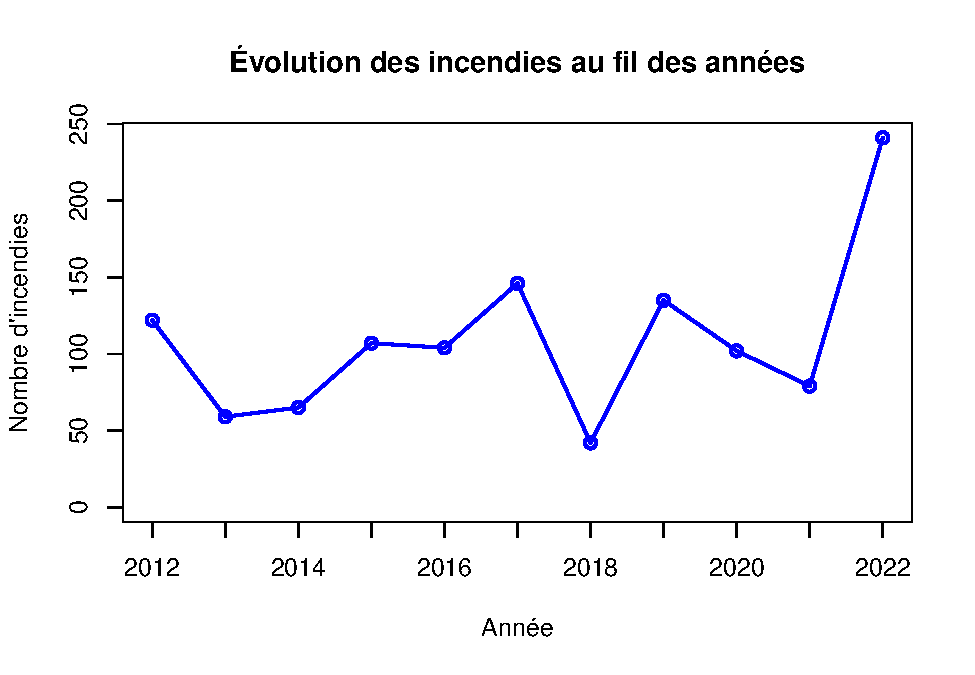
\includegraphics{Rapport_files/figure-latex/setup-1.pdf}

\begin{enumerate}
\def\labelenumi{\arabic{enumi}.}
\tightlist
\item
  \textbf{Analyse Informatique:}
\end{enumerate}

Nous allons détailler le processus de développement du code pour
structurer notre graphique. Pour cela, nous avons importé les données du
fichier grâce à la méthode \textbf{read.csv()}. Dans cette méthode, nous
avons spécifié le chemin relatif du fichier csv.Par la suite, nous avons
déterminé la fréquence des incendies par an en optant pour la colonne
\textbf{donneees\$annee}.En employant la méthode \textbf{table()}, nous
dénombrons le nombre d'incendies survenant par année.

Cela nous autorisera à constituer un tableau où les indices représentent
les années et les valeurs correspondent aux occurrences des incendies.

À présent, nous passons à la création du graphique à l'aide de la
méthode \textbf{plot()}. Nous avons indiqué la variable
\textbf{annee\_freq} et dans cette méthode, nous avons précisé le type
`o' pour indiquer que les points doivent être affichés et reliés par une
ligne. De plus, nous avons défini l'option couleur afin de spécifier que
le graphique doit être en bleu.

Avec l'option \textbf{main}, nous désignons le titre du diagramme.
Ensuite, grâce à xlab et ylab, nous définissons les étiquettes des axes
x et y, où x représente l'\textbf{année} et y représente le
\textbf{nombre d'incendies}.

\begin{enumerate}
\def\labelenumi{\arabic{enumi}.}
\setcounter{enumi}{1}
\tightlist
\item
  \textbf{Analyse Statistique:}
\end{enumerate}

Alors, débutons par cette étude ; nous allons mener notre analyse sur
une période de 11 ans, de 2012 à 2022.

Nous allons donc commencer à dresser le bilan de nos effectifs
d'incendies. En 2012, nous avons enregistré 122 incidents, en 2013, 59
incendies, en 2014, 65 incendies, en 2015, le nombre a grimpé à 107. En
2016, nous avons eu 104 incendies. Pour l'année suivante, en 2017, nous
avons connu une augmentation avec 146 incidents. Puis en 2018, le
chiffre est redescendu à 42 incendies. En 2019, nous avons rapporté 135
incendies et pour l'année suivante, en 2020 nous avions enregistré 102
incidents. Enfin pour2021 ,nous avons comptabilisé 79 incendies et
pour2022 ,le nombre d'incendies a fortement augmenté atteignant
241incendies .

Il est possible d'observer que la moyenne générale des incendies en
France sur une durée de 11 ans s'élève à 109,27. Maintenant que nous
avons compilé les totaux des onze années consécutives, nous allons
détailler notre analyse. En démarrant de 2012, nous constatons un total
de 122 incendies, ce qui pourrait être considéré comme « bon ».
Cependant, cette comparaison est prématurée tant que nous n'avons pas
répertorié les autres chiffres pour une évaluation plus approfondie.
Après une baisse de 63 incendies en 2013, on a constaté une augmentation
de 6 incendies en 2014 lors de la comparaison entre 2013 et 2014.

Cependant, en 2015, le nombre d'incendies a considérablement augmenté,
atteignant 107 incendies pour l'année 2015, ce qui représente un chiffre
élevé mais pas le plus élevé que nous ayons connu. En comparaison avec
2012, nous avons atteint un taux qui est le deuxième record maximal.
Puis en 2016, ce taux a baissé de trois incendies par rapport à l'année
précédente.

En 2017, on a observé une hausse remarquable du taux d'incendies qui a
atteint un nouveau sommet à 146, soit une augmentation de 42 incendies
par rapport à 2016. Si l'on compare avec l'année 2012, cela représente
une différence de 24 incendries. En 2018, on constate une baisse rapide
du nombre d'incendies, enregistrant un taux de 42 qui, selon les données
de 2018, représente le plus bas enregistré depuis 2012. En 2019, on a
noté une hausse significative du nombre d'incendies, atteignant 135,
soit une différence de 93 incendies par rapport à 2018.

En 2020, une baisse du nombre d'incendies entraîne une variation de 33
incendies par rapport à l'année 2029. Ensuite, on observe une baisse en
2021 avec une différence de 23 incendies par rapport à l'année 2020.
Finalement, un chiffre très élevé en 2022 a été atteint, atteignant le
nombre record de 241 incendies. De plus, cela représente une différence
de 162 incendres par rapport à l'année 2021.

On peut résumer qu'au cours de ces 11 années, l'année où le nombre
d'incendies est le plus élevé est 2022 avec un total de 241 incendies,
tandis que l'année où ce nombre est le plus bas est 2018.

En 2022, on a observé une augmentation atypique, avec un total de 241
incendies. Divers éléments peuvent expliquer cette augmentation, tels
que les modifications extrêmes des conditions météorologiques. En 2022,
des vagues de chaleur sévères et une sécheresse persistante ont
contribué à cet accroissement. De plus, les actions humaines, notamment
la négligence, ont influencé cette hausse.

Pour conclure notre analyse, l'évolution des incendies de 2012 à 2022 a
montré des tendances significatives et atypiques. Cela souligne
l'importance d'examiner l'impact des facteurs climatiques, humains et
socio-économiques sur le nombre d'incendies. On peut conclure que
l'année 2022 a été exceptionnelle, affichant le plus haut nombre
d'incendies. De plus, nous avons observé une variabilité des tendances,
comme démontré souvent avec les années 2017, 2014 et 2013 où les taux
étaient remarquablement bas comparés à ceux de 2022. Il est essentiel de
noter que le changement climatique a une grande importance.

Enfin, et c'est crucial, la gestion et la prévention jouent un rôle
primordial. Les préfectures, ainsi que les forces de police municipales
et nationales, peuvent contribuer à maîtriser ce taux d'incendies
attribués à des actes de malveillance ou de négligence.

\subparagraph{4.3.1.2 Analyse des heures
d'incendie}\label{analyse-des-heures-dincendie}

\subparagraph{4.3.1.3 Évolution décennale des causes
d'incendies}\label{uxe9volution-duxe9cennale-des-causes-dincendies}

\subparagraph{4.3.1.4 Heures critiques de
déclenchement}\label{heures-critiques-de-duxe9clenchement}

\subparagraph{4.3.1.5 Cyclicité
hebdomadaire}\label{cyclicituxe9-hebdomadaire}

\paragraph{4.3.2 Facteurs climatiques et
météorologiques}\label{facteurs-climatiques-et-muxe9tuxe9orologiques}

\subparagraph{4.3.2.1 Influence de la température sur les
incendies}\label{influence-de-la-tempuxe9rature-sur-les-incendies}

\subparagraph{4.3.2.2 Impact de l'humidité sur les
incendies}\label{impact-de-lhumidituxe9-sur-les-incendies}

Pour mener l'analyse de l'influence de l'humidité sur les incendies, il
est nécessaire de constituer notre base d'analyse. Il est nécessaire
d'utiliser les deux tables que nous avons mises en place dans notre Base
de données, à savoir la Table Incendies et la Table donnees\_meteo.

Afin de réaliser une jointure entre ces deux tables, nous avons fait
appel à une troisième table nommée humidite qui regroupe les champs des
deux tables visées, partageant un élément en commun : le « Code\_INSEE
». Nous avons détaillé la méthode utilisée pour cela dans la section
Informatique de notre rapport.

Avant d'approfondir dans les détails de notre étude, nous allons d'abord
définir les termes clés que nous utiliserons dans notre analyse.
L'humidité se réfère à la présence de vapeur d'eau dans l'air.

Le but de notre analyse est d'étudier le lien entre l'humidité
atmosphérique et les incendies. Pour accomplir cela, nous devons étudier
la relation entre l'humidité et la dimension des incendies.

\emph{Il est essentiel de mettre en évidence deux attributs importants.}

\begin{enumerate}
\def\labelenumi{\arabic{enumi}.}
\item
  \textbf{Tens\_vap\_med}: Cet attribut évalue la pression de
  vaporisation moyenne, qui est une autre façon de dire qu'il s'agit
  d'un indicateur de l'humidité de l'air.
\item
  \textbf{surface\_parcourue\_m2}: Cette caractéristique présente la
  superficie ravagée par un feu, ce qui en fait un instrument pour
  évaluer l'intensité du feu.
\end{enumerate}

Dans cette étude, nous allons créer et analyser deux graphes
indispensables à notre problématique.

\begin{enumerate}
\def\labelenumi{\arabic{enumi}.}
\tightlist
\item
  \textbf{Histogramme de l'humidité}
\end{enumerate}

Le diagramme de l'humidité nous aidera à examiner et à saisir la
distribution des taux d'humidité dans l'échantillon de données.

L'humidité joue un rôle crucial dans l'analyse des incendies en raison
de son impact sur la rapidité de leur avancement. Cependant, avant
d'examiner toute relation avec la surface incendiée, nous devons d'abord
comprendre comment l'humidité fluctue dans les données.

\begin{Shaded}
\begin{Highlighting}[]
\FunctionTok{library}\NormalTok{(ggplot2)}
\NormalTok{data }\OtherTok{\textless{}{-}} \FunctionTok{read.csv}\NormalTok{(}\StringTok{"../Exports/export\_Humidites.csv"}\NormalTok{)}
\FunctionTok{ggplot}\NormalTok{(data, }\FunctionTok{aes}\NormalTok{(}\AttributeTok{x =}\NormalTok{ Tens\_vap\_med)) }\SpecialCharTok{+}
  \FunctionTok{geom\_histogram}\NormalTok{(}\AttributeTok{binwidth =} \FloatTok{0.5}\NormalTok{, }\AttributeTok{fill =} \StringTok{"\#1f77b4"}\NormalTok{, }\AttributeTok{color =} \StringTok{"white"}\NormalTok{, }\AttributeTok{alpha =} \FloatTok{0.7}\NormalTok{) }\SpecialCharTok{+}
  \FunctionTok{labs}\NormalTok{(}\AttributeTok{title =} \StringTok{"Distribution de l\textquotesingle{}humidité de l\textquotesingle{}air (Tens\_vap\_med)"}\NormalTok{, }
       \AttributeTok{x =} \StringTok{"Humidité de l\textquotesingle{}air (Tens\_vap\_med)"}\NormalTok{, }
       \AttributeTok{y =} \StringTok{"Fréquence"}\NormalTok{) }\SpecialCharTok{+}
  \FunctionTok{theme\_minimal}\NormalTok{()}
\end{Highlighting}
\end{Shaded}

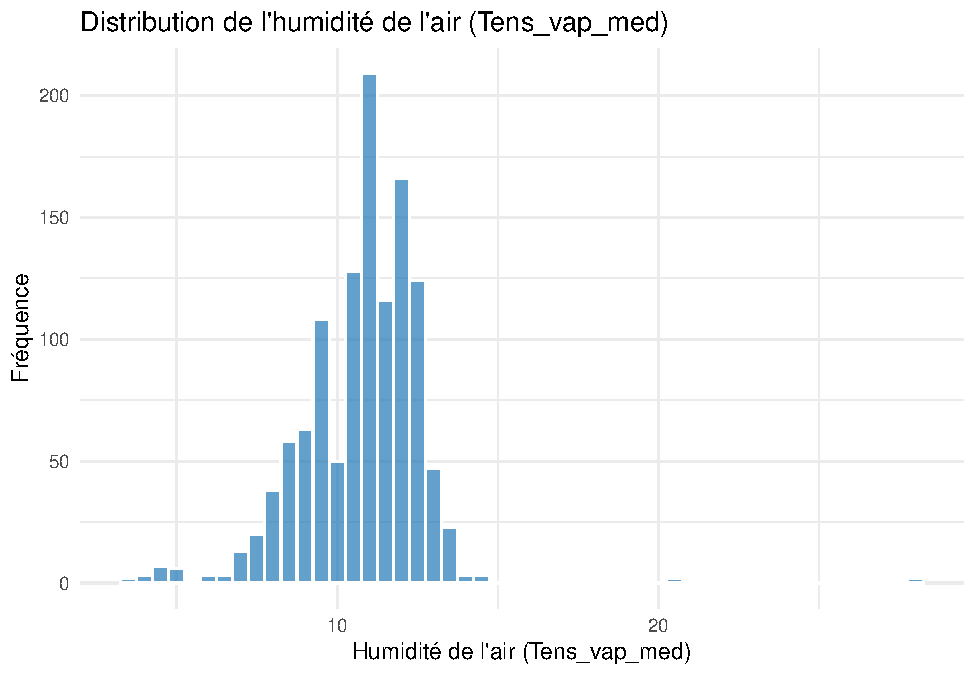
\includegraphics{Rapport_files/figure-latex/unnamed-chunk-1-1.pdf}

\begin{enumerate}
\def\labelenumi{\arabic{enumi}.}
\tightlist
\item
  \textbf{Analyse Informatique:}
\end{enumerate}

Dans notre code destiné à la création du graphique, nous avons employé
le langage R pour sa réalisation. Tout d'abord, nous avons importé le
fichier en utilisant la méthode \textbf{read.csv()}.

Par la suite, on procède à l'initialisation du graphique que l'on
souhaite concevoir avec la méthode \textbf{ggplot()}.On passe en
paramètres de cette méthode les données ainsi que l'\textbf{aes},qui
nous permet de spécifier que l'axe des x sera représenté par
\textbf{Tens\_vap\_med}.

On définit ensuite une autre méthode \textbf{geom\_histogram()} pour
intégrer un histogramme au graphique. Dans cette méthode, on spécifie
des paramètres pour déterminer la largeur des barres de l'histogramme,
et par la suite, on remplit les barres en bleu. Nous définissons la
bordure en blanc et rendons les barres davantage transparentes.

On détermine les titres et étiquettes en faisant appel à la méthode
\textbf{labs()}, en exploitant les paramètres title, x et y.Le titre
indique le sujet du graphique, `x' correspond à l'étiquette de l'axe
horizontal et `y' correspond à l'étiquette de l'axe vertical.

Et pour donner un aspect minimaliste au thème, nous avons employé la
méthode \textbf{theme\_minimal()} afin d'incorporer un style plus
contemporain.

\begin{enumerate}
\def\labelenumi{\arabic{enumi}.}
\setcounter{enumi}{1}
\tightlist
\item
  \textbf{Analyse Statistique:}
\end{enumerate}

L'axe des abscisses illustre l'humidité de l'air, déterminée par la
pression de vapeur moyenne. Les chiffres se situent approximativement
entre 0 et 25.On présume que les valeurs sont exprimées en hPa. C'est
une unité utilisée pour évaluer la pression de la vapeur.

L'axe ordonnes illustre la fréquence, c'est-à-dire le total des
observations pour chaque plage de tension de vapeur. Il a atteint une
fréquence maximale de 200.

D'après les informations intégrées, cet histogramme révèle une
distribution asymétrique avec une importante concentration de valeurs
faibles en matière d'humidité de l'air, allant de 5 à 15 hPa.

L'histogramme présente une asymétrie vers la droite, avec un grand
nombre d'observations ayant de faibles valeurs de tension de vapeur,
indiquant une humidité faible à modérée, et quelques observations à des
valeurs plus élevées, traduisant une humidité supérieure.

On pourrait affirmer que la classe modale de cet histogramme se situe
approximativement entre 10 et 12 hPa.

La portée de cet histogramme s'étend de 0 à 25 hPa. Néanmoins, on
remarque qu'il existe très peu de données entre 20 et 25 hPa. De plus,
il est évident qu'au-delà de 22 hPa, aucune observation n'est présente.

Dans notre histogramme, on peut observer la présence d'une longue queue,
bien qu'elle soit peu dense. Autrement dit, cela nous indique que les
valeurs élevées de tension de vapeur sont peu fréquentes dans cet
ensemble de données.

Nous allons déterminer les interprétations des intervalles concernant le
taux d'humidité.

\begin{enumerate}
\def\labelenumi{\arabic{enumi}.}
\tightlist
\item
  \textbf{0 a 5 hPa}: Cette plage indique un taux d'humidité très bas.
\item
  \textbf{5 a 15 hPa}: C'est la zone où est rassemblée la plupart des
  données. La fréquence s'accroît rapidement dès que l'on atteint 5 hPa,
  atteignant un maximum aux alentours de 10 à 12 hPa avant de
  redescendre. Cela signifie que le niveau d'humidité est modéré.
\item
  \textbf{15 a 20 hPa}:Dans cette période, nous observons une réduction
  qui est associée à des conditions plus humides.
\item
  \textbf{20 a 25 hPa}:Les observations sont peu fréquentes. La
  fréquence étant pratiquement de 0, on peut observer que nous avons des
  conditions hors du commun, telles que des climats tropicaux.
\end{enumerate}

Dans un cadre météorologique, la tension de vapeur représente une
évaluation de la pression partielle de la vapeur d'eau dans
l'atmosphère, liée directement à l'humidité. Selon notre histogramme,
une pression de vapeur de 10 hPa est associée à une humidité relative
modérée, tandis qu'une pression de vapeur avoisinant les 20 hPa indique
un niveau d'humidité considérablement plus élevé, potentiellement proche
de la saturation.

Cet histogramme indiquant une concentration autour de 10-12 hPA suggère
un climat tempéré, caractérisé par une humidité généralement modérée la
majorité du temps, mais avec des périodes plus humides de manière
sporadique.

\begin{enumerate}
\def\labelenumi{\arabic{enumi}.}
\setcounter{enumi}{1}
\tightlist
\item
  \textbf{Diagrame de dispersion}
\end{enumerate}

Ce schéma nous offre la possibilité d'examiner s'il y a une relation
entre l'humidité atmosphérique et l'étendue des incendies (autrement
dit, la superficie qu'ils couvrent).

L'objectif est d'observer comment l'humidité influe sur la taille des
incendies de manière perceptible.

\begin{Shaded}
\begin{Highlighting}[]
\FunctionTok{library}\NormalTok{(ggplot2)}
\NormalTok{data }\OtherTok{\textless{}{-}} \FunctionTok{read.csv}\NormalTok{(}\StringTok{"../Exports/export\_Humidites.csv"}\NormalTok{)}
\FunctionTok{ggplot}\NormalTok{(data, }\FunctionTok{aes}\NormalTok{(}\AttributeTok{x =}\NormalTok{ Tens\_vap\_med, }\AttributeTok{y =}\NormalTok{ surface\_parcourue\_m2)) }\SpecialCharTok{+}
  \FunctionTok{geom\_point}\NormalTok{(}\FunctionTok{aes}\NormalTok{(}\AttributeTok{color =}\NormalTok{ surface\_parcourue\_m2), }\AttributeTok{size =} \DecValTok{2}\NormalTok{, }\AttributeTok{alpha =} \FloatTok{0.7}\NormalTok{) }\SpecialCharTok{+} 
  \FunctionTok{scale\_color\_gradient}\NormalTok{(}\AttributeTok{low =} \StringTok{"blue"}\NormalTok{, }\AttributeTok{high =} \StringTok{"red"}\NormalTok{) }\SpecialCharTok{+} 
  \FunctionTok{labs}\NormalTok{(}\AttributeTok{title =} \StringTok{"Relation entre l\textquotesingle{}humidité de l\textquotesingle{}air et la surface parcourue par les incendies"}\NormalTok{, }
       \AttributeTok{x =} \StringTok{"Humidité de l\textquotesingle{}air (Tens\_vap\_med)"}\NormalTok{, }
       \AttributeTok{y =} \StringTok{"Surface parcourue par les incendies (m²)"}\NormalTok{) }\SpecialCharTok{+}
  \FunctionTok{theme\_minimal}\NormalTok{()}
\end{Highlighting}
\end{Shaded}

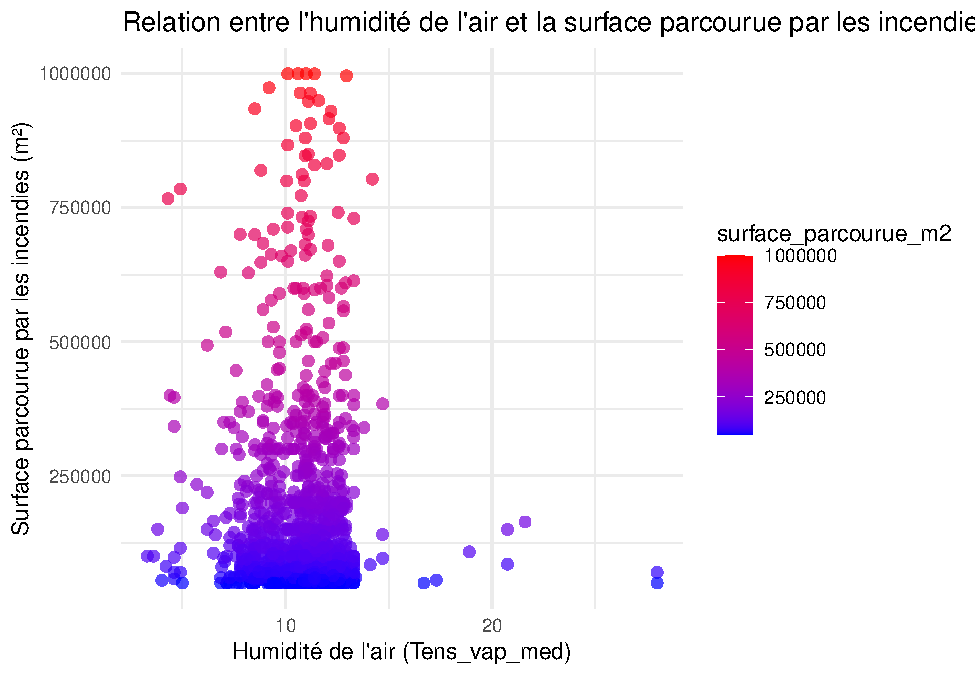
\includegraphics{Rapport_files/figure-latex/unnamed-chunk-2-1.pdf}

Dans ce diagramme, seul l'axe des X représente l'air mesuré par la
tension de vapeur moyenne. Les valeurs varient de 0 à 25 hPa. L'axe des
Y représente la superficie parcourue par les incendies, exprimée en
mètres carrés.

Nous avons choisi d'utiliser un graphique de type nuage de points,
également appelé \textbf{scatter plot}, où chaque point représente une
observation (incendie) associée à deux variables. Premièrement, il
s'agit de l'humidité atmosphérique au moment du sinistre, et en second
lieu, de la superficie affectée par cet incendie (Y).

La couleur des points varie du bleu au rouge, conformément à l'échelle
indiquée sur la droite. Les points bleus représentent des surfaces
inférieures à 250 000 m², alors que les points rouges sont associés à
des surfaces supérieures.

Débutons par l'étude de la répartition des points, en mettant d'abord
l'accent sur leur concentration. La plupart des points se regroupent
dans la plage d'humidité de 0 à 15 hPa, avec une densité
particulièrement élevée entre 5 et 12 hPa. Cela entraîne des niveaux
d'humidité modérés.

On remarque également que le nombre de points au-delà de 20 hPa est très
limité, ce qui suggère que les incendies dans des conditions extrêmement
humides sont rares.

En ce qui concerne la superficie affectée par les incendies, allant de 0
à 250 000 m², on remarque que la majorité d'entre eux ont une portée
assez restreinte. Pour les surfaces allant jusqu'à 1 000 000 m2, le
graphique semble indiquer que les incendies de plus grande ampleur sont
moins communs.

Concernant le lien entre l'humidité et la surface parcourue, on remarque
une concentration de points bleus dans l'intervalle d'humidité de 5 à 15
hPa. Cela indique que les incendies de faible envergure se produisent
plus souvent dans des conditions d'humidité modérées. En ce qui concerne
les points rouges, ils sont plus éparpillés et se situent dans la même
fourchette, bien qu'il existe des points rouges dans des zones où
l'humidité est à la fois plus basse et plus élevée.

On ne constate pas de lien clair et direct entre le taux d'humidité de
l'air et la superficie touchée par les feux. Les feux de grande
envergure (indiqués par des points rouges) surviennent à divers niveaux
d'humidité, toutefois, la plupart d'entre eux (qu'ils soient petits ou
grands) se regroupent dans l'intervalle de 5 à 15 hPa.

Cependant, une tendance mineure peut être observée : les incendies de
plus grande envergure (près de 1 000 000 m²) ont l'air de survenir un
peu plus fréquemment dans des conditions d'humidité plus basse (environ
5 hPa ou moins), où l'air est plus sec, ce qui facilite la diffusion des
flammes. Néanmoins, cette tendance n'est pas très prononcée.

\begin{enumerate}
\def\labelenumi{\arabic{enumi}.}
\setcounter{enumi}{2}
\tightlist
\item
  \textbf{Comparaison avec l'histograme precedent:}
\end{enumerate}

L'histogramme précédent nous indiquait que la pression de vapeur moyenne
se situait approximativement entre 5 et 15 hPa, avec un sommet autour de
10-12 hPa. Cette distribution est confirmée par ce nuage de points.

Les quelques rares points au-delà de 20 hPa dans l'histogramme
témoignent de la confirmation que les incendies sont peu fréquents dans
des conditions très humides.

\begin{enumerate}
\def\labelenumi{\arabic{enumi}.}
\setcounter{enumi}{3}
\tightlist
\item
  \textbf{Analyse Statistique}
\end{enumerate}

Après avoir réalisé l'analyse des deux graphiques, nous sommes en mesure
d'effectuer une analyse statistique.

Nous allons effectuer un calcul de corrélation.Elle nous offrira la
possibilité d'évaluer l'intensité et le sens de la corrélation linéaire
entre l'humidité atmosphérique et les dimensions des feux.

Avant tout, définissons les choses. Il s'agit d'une mesure statistique
qui illustre la force et la direction d'un lien entre deux variables.
Elle nous aide, de manière simple, à saisir comment deux variables se
déplacent l'une par rapport à l'autre. On utilise le coefficient de
corrélation de Pearson, qui se situe entre -1 et 1, pour quantifier la
corrélation. Avec 1 représentant une corrélation parfaitement positive,
-1 une corrélation parfaitement négative et 0 signifiant aucune
corrélation.

\begin{Shaded}
\begin{Highlighting}[]
\NormalTok{correlation }\OtherTok{\textless{}{-}} \FunctionTok{cor}\NormalTok{(data}\SpecialCharTok{$}\NormalTok{Tens\_vap\_med, data}\SpecialCharTok{$}\NormalTok{surface\_parcourue\_m2, }\AttributeTok{use =} \StringTok{"complete.obs"}\NormalTok{)}
\FunctionTok{print}\NormalTok{(}\FunctionTok{paste}\NormalTok{(}\StringTok{"Corrélation entre Tens\_vap\_med et surface\_parcourue\_m2: "}\NormalTok{, correlation))}
\end{Highlighting}
\end{Shaded}

\begin{verbatim}
## [1] "Corrélation entre Tens_vap_med et surface_parcourue_m2:  -0.0211442157372533"
\end{verbatim}

Dans ce code, nous avons fait appel à la fonction « cor() » afin de
déterminer la corrélation de Pearson entre Tens\_vap\_med et
surface\_parcourue\_m2, en omettant les variables manquantes. La méthode
cor() nous donnera un coefficient de corrélation, comme expliqué
précédemment.

\begin{enumerate}
\def\labelenumi{\arabic{enumi}.}
\item
  Si la corrélation est haute, proche de 1, cela nous permet d'affirmer
  qu'une hausse de l'humidité est liée à une extension des incendies.
\item
  Si la corrélation est négative (proche de -1), cela implique qu'une
  hausse de l'humidité est liée à une réduction de la grandeur des feux.
\item
  Une corrélation proche de 0 suggère l'absence d'une relation linéaire
  manifeste.
\end{enumerate}

L'analyse de corrélation révèle qu'il n'existe pas de lien linéaire
prononcé entre le taux d'humidité et l'ampleur des feux dans vos
informations. Selon cette étude, l'humidité semble avoir une influence
marginale sur l'ampleur des incendies.

Apres avoir calcule la correlation on va y tracer le graphe de cette
correlation

\begin{Shaded}
\begin{Highlighting}[]
\FunctionTok{library}\NormalTok{(ggplot2)}
\NormalTok{data }\OtherTok{\textless{}{-}} \FunctionTok{read.csv}\NormalTok{(}\StringTok{"../Exports/export\_Humidites.csv"}\NormalTok{)}
\FunctionTok{ggplot}\NormalTok{(data, }\FunctionTok{aes}\NormalTok{(}\AttributeTok{x =}\NormalTok{ Tens\_vap\_med, }\AttributeTok{y =}\NormalTok{ surface\_parcourue\_m2)) }\SpecialCharTok{+}
  \FunctionTok{geom\_point}\NormalTok{(}\AttributeTok{color =} \StringTok{"blue"}\NormalTok{, }\AttributeTok{alpha =} \FloatTok{0.6}\NormalTok{) }\SpecialCharTok{+}  \CommentTok{\# Ajoute les points}
  \FunctionTok{geom\_smooth}\NormalTok{(}\AttributeTok{method =} \StringTok{"lm"}\NormalTok{, }\AttributeTok{color =} \StringTok{"red"}\NormalTok{, }\AttributeTok{se =} \ConstantTok{FALSE}\NormalTok{) }\SpecialCharTok{+}  \CommentTok{\# Ajoute la droite de régression}
  \FunctionTok{labs}\NormalTok{(}\AttributeTok{title =} \StringTok{"Corrélation entre Force du Vent et Surface Parcourue"}\NormalTok{,}
       \AttributeTok{x =} \StringTok{"Tens\_vap\_med (moyenne)"}\NormalTok{,}
       \AttributeTok{y =} \StringTok{"Surface Parcourue (m²)"}\NormalTok{) }\SpecialCharTok{+}
  \FunctionTok{theme\_minimal}\NormalTok{()}
\end{Highlighting}
\end{Shaded}

\begin{verbatim}
## `geom_smooth()` using formula = 'y ~ x'
\end{verbatim}

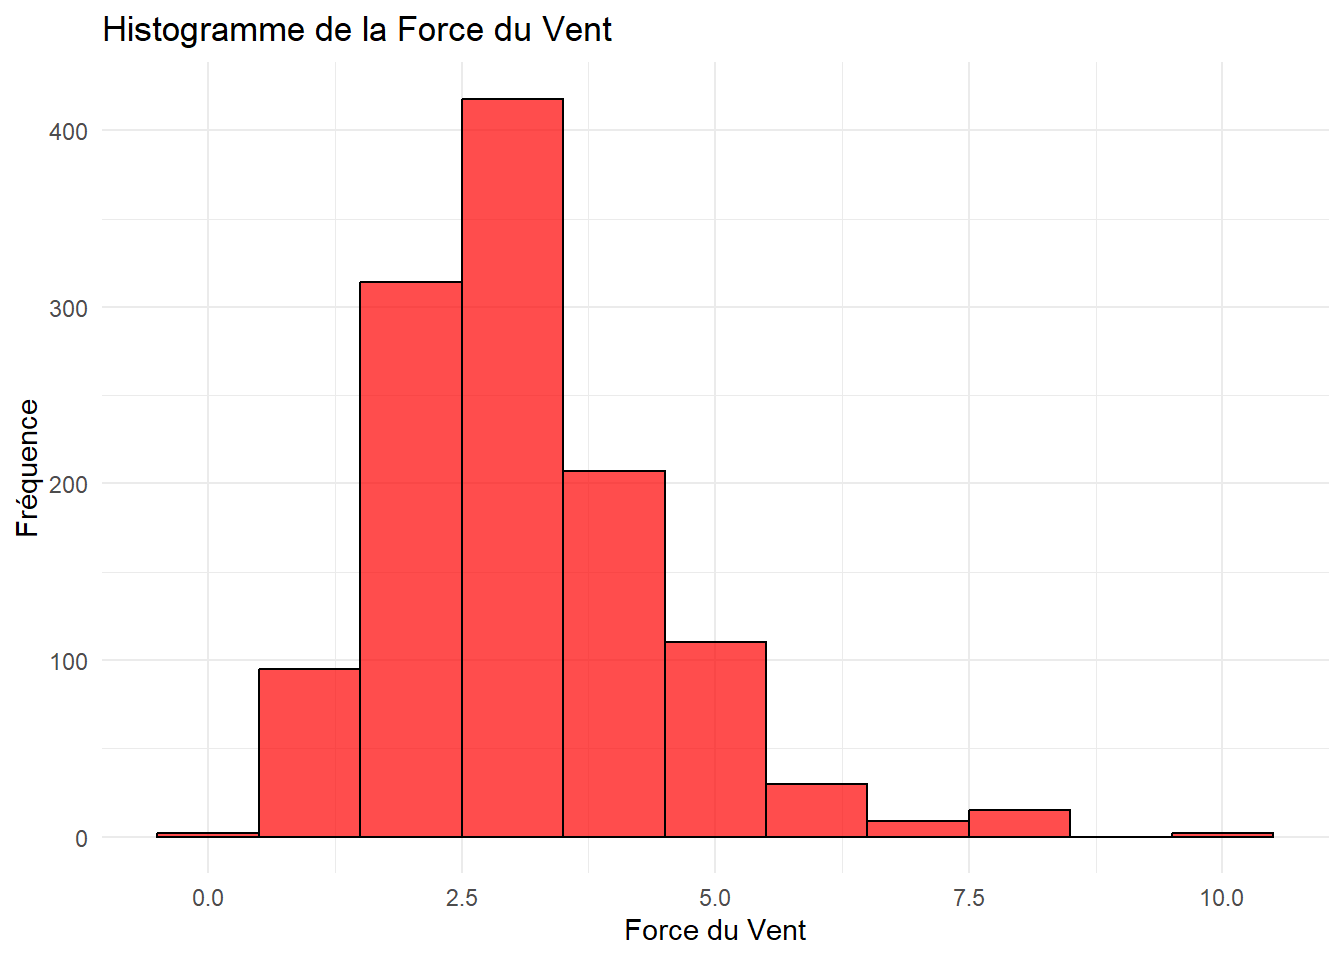
\includegraphics{Rapport_files/figure-latex/unnamed-chunk-4-1.pdf}

\subparagraph{4.3.2.3 Relation entre le vent et la propagation des
incendies}\label{relation-entre-le-vent-et-la-propagation-des-incendies}

Pour examiner la question relative à la corrélation entre le vent et la
diffusion des incendies sur le sol français, nous adopterons une
approche distincte en segmentant ce sujet en quatres sous-questions.

C'est pourquoi, pour aborder ce problème, on devrait considérer ces cinq
enjeux :

\begin{enumerate}
\def\labelenumi{\arabic{enumi}.}
\tightlist
\item
  Force du vent
\item
  Surface parcourue par le feu en fonction de la Force du vent
\item
  Force du vent par zone géographique
\item
  Surface parcourue par le feu par zone géographique
\end{enumerate}

Avant d'examiner les quatre sous-problèmes, nous allons inspecter la
corrélation.Nous pourrions vérifier la corrélation entre la puissance du
vent et la surface parcourue en mètres carrés. En procédant ainsi, nous
pourrions déterminer s'il existe une relation linéaire entre ces deux
variables.

On remarque donc que si le coefficient de corrélation se rapproche de -1
ou 1, cela signifie qu'il existe une relation linéaire significative
entre ces deux variables.

\begin{Shaded}
\begin{Highlighting}[]
\NormalTok{data }\OtherTok{\textless{}{-}} \FunctionTok{read.csv}\NormalTok{(}\StringTok{"../Exports/export\_vents.csv"}\NormalTok{)}
\FunctionTok{cor}\NormalTok{(data}\SpecialCharTok{$}\NormalTok{Force\_vent\_med, data}\SpecialCharTok{$}\NormalTok{surface\_parcourue\_m2, }\AttributeTok{use =} \StringTok{"complete.obs"}\NormalTok{)}
\end{Highlighting}
\end{Shaded}

\begin{verbatim}
## [1] 0.03137438
\end{verbatim}

Puisque le coefficient de corrélation de Pearson est proche de 0, cela
indique qu'il n'existe pas de relation linéaire significative entre les
deux variables.

Pour une perspective plus statistique, nous allons essayer la régression
polynomiale.C'est une technique employée pour modéliser le lien entre
une variable indépendante, comme dans notre situation la puissance du
véhicule, et une variable dépendante, ici la distance parcourue par le
feu, à condition que ce lien ne soit pas linéaire. Cela s'applique à
notre situation.

Cela nous offre la possibilité de mieux saisir les courbures ou les
tendances complexes des données, contrairement à une régression linéaire
simple qui postule une relation proportionnelle constante entre les deux
variables.

Dans ce contexte, nous employons une régression polynomiale de degré 2,
que l'on peut également qualifier de régression quadratique.Cette
dernière intègre finalement le terme linéaire (force du vent) ainsi que
le terme quadratique (force du vent au carré).

On va détailler davantage pourquoi nous avons opté pour une régression
polynomiale, étant donné qu'elle nous offre la possibilité de saisir des
relations non linéaires entre les variables.Une condition est établie si
le lien entre la puissance du vent et la superficie touchée par le feu
suit une courbe, comme c'est le cas dans notre scénario, avec une
accélération rapide initiale qui se ralentit à mesure que la force du
vent s'intensifie.Dans ce contexte, une régression polynomiale serait
plus appropriée qu'une régression linéaire simple.

\begin{Shaded}
\begin{Highlighting}[]
\FunctionTok{library}\NormalTok{(ggplot2)}

\CommentTok{\# Charger les données}
\NormalTok{data }\OtherTok{\textless{}{-}} \FunctionTok{read.csv}\NormalTok{(}\StringTok{"../Exports/export\_vents.csv"}\NormalTok{)}

\CommentTok{\# Créer un graphique avec régression polynomial}
\FunctionTok{ggplot}\NormalTok{(data, }\FunctionTok{aes}\NormalTok{(}\AttributeTok{x =}\NormalTok{ Force\_vent\_med, }\AttributeTok{y =}\NormalTok{ surface\_parcourue\_m2)) }\SpecialCharTok{+}
  \FunctionTok{geom\_point}\NormalTok{(}\AttributeTok{color =} \StringTok{"black"}\NormalTok{, }\AttributeTok{size =} \DecValTok{2}\NormalTok{) }\SpecialCharTok{+} 
  \FunctionTok{geom\_smooth}\NormalTok{(}\AttributeTok{method =} \StringTok{"lm"}\NormalTok{, }\AttributeTok{formula =}\NormalTok{ y }\SpecialCharTok{\textasciitilde{}} \FunctionTok{poly}\NormalTok{(x, }\DecValTok{2}\NormalTok{), }\AttributeTok{color =} \StringTok{"blue"}\NormalTok{, }\AttributeTok{se =} \ConstantTok{FALSE}\NormalTok{) }\SpecialCharTok{+} 
  \FunctionTok{labs}\NormalTok{(}\AttributeTok{title =} \StringTok{"Régression Polynomial"}\NormalTok{, }
       \AttributeTok{x =} \StringTok{"Force du Vent"}\NormalTok{, }
       \AttributeTok{y =} \StringTok{"Surface Parcourue (m²)"}\NormalTok{) }\SpecialCharTok{+}
  \FunctionTok{theme\_minimal}\NormalTok{()}
\end{Highlighting}
\end{Shaded}

\includegraphics{Rapport_files/figure-latex/unnamed-chunk-6-1.pdf}

Nous allons détailler, à travers une analyse informatique, la manière
dont nous avons réalisé la régression polynomiale.Pour cela, nous avons
utilisé la méthode \textbf{geom\_smooth()}, accompagnée de l'argument
\textbf{method = ``lm''} qui indique que nous sommes en présence d'un
modèle de régression.La formule = y \textasciitilde{} poly(x, 2) précise
qu'il s'agit d'une régression polynomiale de degré 2 (quadratique).

Nous allons pouvoir intégrer une courbe de régression linéaire grâce à
la méthode \textbf{geom\_smooth(method = ``lm'')}. L'indication précise
que le modèle repose sur une analyse de régression linéaire.

Cette spécification, \textbf{formula = y \textasciitilde{} poly(x, 2)},
indique au langage R que nous souhaitons un modèle polynomial du second
degré. \textbf{poly(x, 2)} est une fonction qui produit les termes x et
x\^{}2, représentant respectivement la vitesse du vent et son carré.Cela
permettra à la régression de s'ajuster à la fois à une pente linéaire et
à une courbure quadratique des données.

L'attribut \textbf{color=``blue''} nous offre la possibilité de peindre
la courbe de régression en bleu, ce qui permet une distinction claire
avec les autres éléments du graphe. Et en outre, \textbf{se=FALSE} nous
permettra de désactiver l'affichage de la marge d'erreur autour de la
courbe de régression.

\begin{enumerate}
\def\labelenumi{\arabic{enumi}.}
\tightlist
\item
  \textbf{Force du vent}
\end{enumerate}

Dans cette sous-problematique on va analyser la force du vent:

\begin{Shaded}
\begin{Highlighting}[]
\FunctionTok{library}\NormalTok{(ggplot2)}
\NormalTok{data }\OtherTok{\textless{}{-}} \FunctionTok{read.csv}\NormalTok{(}\StringTok{"../Exports/export\_vents.csv"}\NormalTok{)}
\FunctionTok{ggplot}\NormalTok{(data, }\FunctionTok{aes}\NormalTok{(}\AttributeTok{x =}\NormalTok{ Force\_vent\_med)) }\SpecialCharTok{+}
  \FunctionTok{geom\_histogram}\NormalTok{(}\AttributeTok{binwidth =} \DecValTok{1}\NormalTok{, }\AttributeTok{fill =} \StringTok{"red"}\NormalTok{, }\AttributeTok{color =} \StringTok{"black"}\NormalTok{, }\AttributeTok{alpha =} \FloatTok{0.7}\NormalTok{) }\SpecialCharTok{+}
  \FunctionTok{labs}\NormalTok{(}\AttributeTok{title =} \StringTok{"Histogramme de la Force du Vent"}\NormalTok{, }\AttributeTok{x =} \StringTok{"Force du Vent"}\NormalTok{, }\AttributeTok{y =} \StringTok{"Fréquence"}\NormalTok{) }\SpecialCharTok{+}
  \FunctionTok{theme\_minimal}\NormalTok{()}
\end{Highlighting}
\end{Shaded}

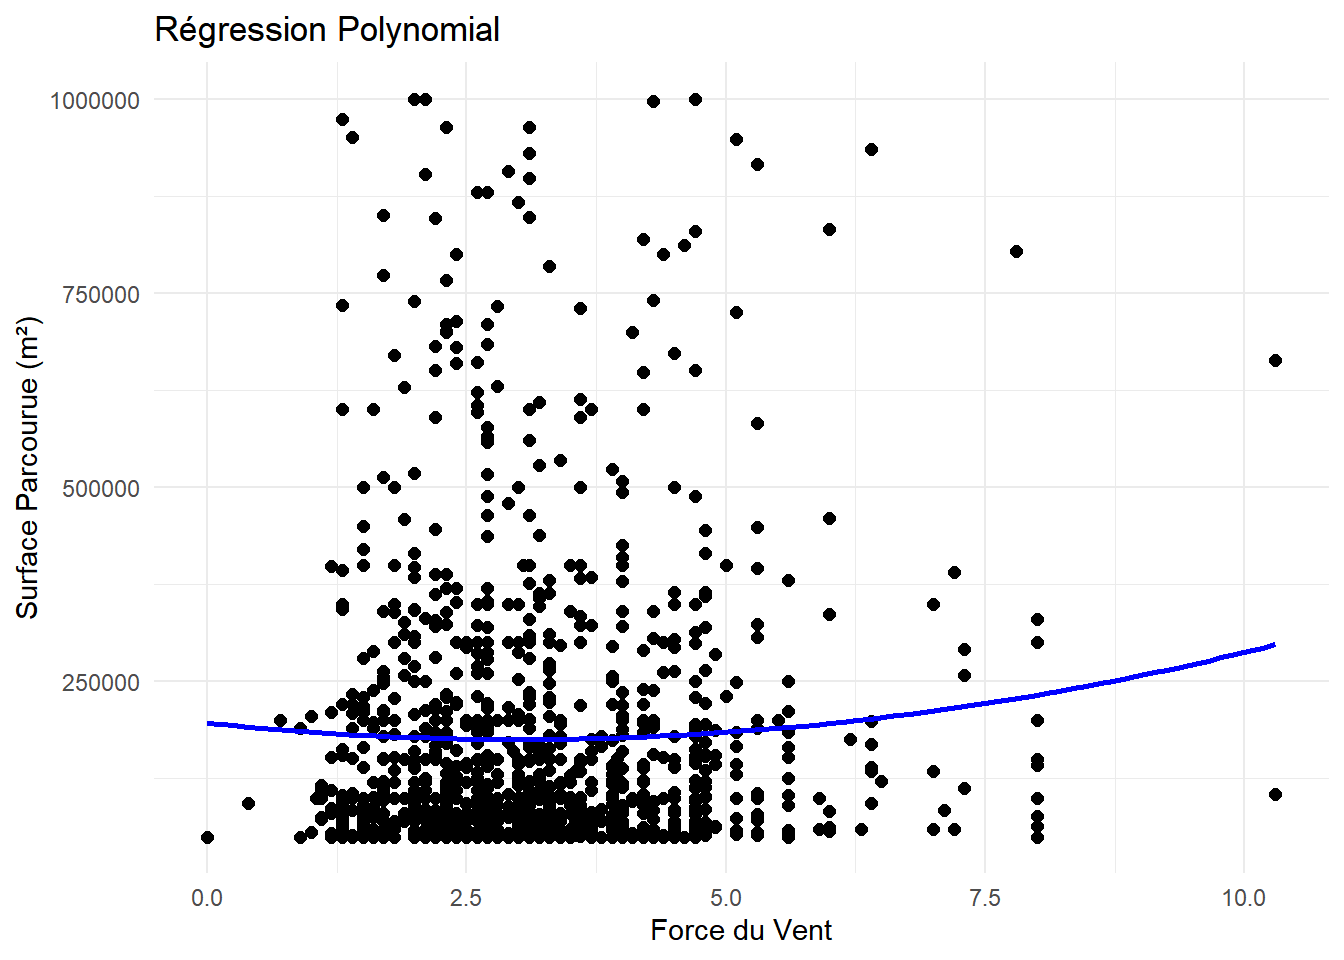
\includegraphics{Rapport_files/figure-latex/unnamed-chunk-7-1.pdf}

\begin{enumerate}
\def\labelenumi{\arabic{enumi}.}
\tightlist
\item
  \textbf{Analyse Informatique:}
\end{enumerate}

Tout d'abord, nous allons détailler la méthode de construction de notre
graphique. Nous avons utilisé la bibliothèque ggplot du langage R pour
élaborer cet histogramme.Ensuite, nous avons importé nos données en
spécifiant le chemin relatif du fichier CSV que nous avons conçu et
développé à l'aide du langage Python et de la gestion des fichiers.

Dans le processus de chargement du fichier, nous avons employé la
méthode read.csv pour interpréter le fichier CSV, et nous avons
enregistré ces informations dans la variable data.

Par la suite, nous avons fait appel à la méthode, définie dans la
bibliothèque ggplot2, soit la méthode ggplot. Nous lui avons précisé
l'emplacement des données stockées et mis en place une autre méthode
aes, signifiant \textbf{aesthetics}, pour indiquer quelles colonnes de
données devraient être visualisées sur les axes. Dans notre situation,
nous attribuons l'axe des x à la variable Force\_vent\_med qui va
symboliser l'intensité du vent mesurée.

Par la suite, nous employons la méthode \textbf{geom\_histogram()} pour
intégrer l'histogramme à la représentation graphique. Nous spécifions la
largeur des barres, la teinte que nous voulons utiliser pour leur
remplissage, la nuance du contour et également le degré de transparence
des barres.

On termine par la définition des étiquettes et des titres de notre
histogramme grâce à la méthode \textbf{labs()}. On y inclut le titre du
graphique ainsi que les libellés pour les deux axes, x et y. De plus,
comme nous avons opté pour un style minimaliste, nous avons utilisé la
méthode \textbf{theme\_minimal()} afin de conférer un aspect plus
contemporain au graphique.

\begin{enumerate}
\def\labelenumi{\arabic{enumi}.}
\setcounter{enumi}{1}
\tightlist
\item
  \textbf{Analyse Statistique:}
\end{enumerate}

On présume que la force du vent est évaluée en kilomètres par heure.

Cette histograme represente la distribution de la force du vent mesure
en Km/h. L'échelle horizontale montre la puissance du vent, avec des
valeurs variant de 0 à 10,5.L'axe des y symbolise la fréquence, soit le
nombre d'apparitions de chaque plage de force du vent, avec des valeurs
se situant approximativement entre 0 et 400.

L'histogramme indique une distribution asymétrique vers la droite, ce
qui implique une concentration accrue de données pour des valeurs
faibles de la force du vent, avec une longue traîne vers les valeurs
plus élevées.

Le sommet de l'histogramme se trouve approximativement dans la gamme de
3.5 à 4.0 pour la force du vent, avec une fréquence avoisinant les 400.
Cela nous indique que dans cet échantillon, la force du vent la plus
courante se situe dans cette plage.

Concernant la portée des valeurs, la force du vent varie
approximativement de 0 à 10,5. Toutefois, les occurrences de valeurs
dépassant 8 sont extrêmement rares, ce qui indique que de très forts
vents sont peu fréquents dans cet ensemble de données.

Presque 80\% des données se regroupent entre 0 et 5.5 environ, ce qui
indique que cet échantillon est principalement dominé par les vents
légers à modérés.

La moyenne de cet histogramme se situe légèrement au-dessus du mode,
estimée approximativement entre 4.0 et 4.5.Concernant la médiane, elle
se positionne probablement autour de 3.5, car la distribution penche
vers la droite, divisant l'échantillon en deux segments égaux.

Cet histogramme pourrait illustrer des relevés de la puissance du vent
sur une période déterminée.La prévalence de brises légères à modérées
(0.0 à 5.5) indique un climat plutôt paisible, avec la présence
exceptionnelle de vents puissants au-delà de 8, qui pourraient survenir
lors d'événements rares associés à des phénomènes météorologiques tels
que des tempêtes.

Maintenant on va tracer une courbe de densite:

\begin{Shaded}
\begin{Highlighting}[]
\CommentTok{\# Histogramme avec courbe de densité pour la Force du Vent}
\NormalTok{data }\OtherTok{\textless{}{-}} \FunctionTok{read.csv}\NormalTok{(}\StringTok{"../Exports/export\_vents.csv"}\NormalTok{)}
\FunctionTok{ggplot}\NormalTok{(data, }\FunctionTok{aes}\NormalTok{(}\AttributeTok{x =}\NormalTok{ Force\_vent\_med)) }\SpecialCharTok{+}
  \FunctionTok{geom\_histogram}\NormalTok{(}\FunctionTok{aes}\NormalTok{(}\AttributeTok{y =}\NormalTok{ ..density..), }\AttributeTok{binwidth =} \DecValTok{1}\NormalTok{, }\AttributeTok{fill =} \StringTok{"red"}\NormalTok{, }\AttributeTok{color =} \StringTok{"black"}\NormalTok{, }\AttributeTok{alpha =} \FloatTok{0.7}\NormalTok{) }\SpecialCharTok{+}
  \FunctionTok{geom\_density}\NormalTok{(}\AttributeTok{color =} \StringTok{"blue"}\NormalTok{, }\AttributeTok{size =} \DecValTok{1}\NormalTok{) }\SpecialCharTok{+} 
  \FunctionTok{labs}\NormalTok{(}\AttributeTok{title =} \StringTok{"Distribution de la Force du Vent avec Courbe de Densité"}\NormalTok{, }\AttributeTok{x =} \StringTok{"Force du Vent"}\NormalTok{, }\AttributeTok{y =} \StringTok{"Densité"}\NormalTok{) }\SpecialCharTok{+}
  \FunctionTok{theme\_minimal}\NormalTok{()}
\end{Highlighting}
\end{Shaded}

\begin{verbatim}
## Warning: Using `size` aesthetic for lines was deprecated in ggplot2 3.4.0.
## i Please use `linewidth` instead.
## This warning is displayed once every 8 hours.
## Call `lifecycle::last_lifecycle_warnings()` to see where this warning was
## generated.
\end{verbatim}

\begin{verbatim}
## Warning: The dot-dot notation (`..density..`) was deprecated in ggplot2 3.4.0.
## i Please use `after_stat(density)` instead.
## This warning is displayed once every 8 hours.
## Call `lifecycle::last_lifecycle_warnings()` to see where this warning was
## generated.
\end{verbatim}

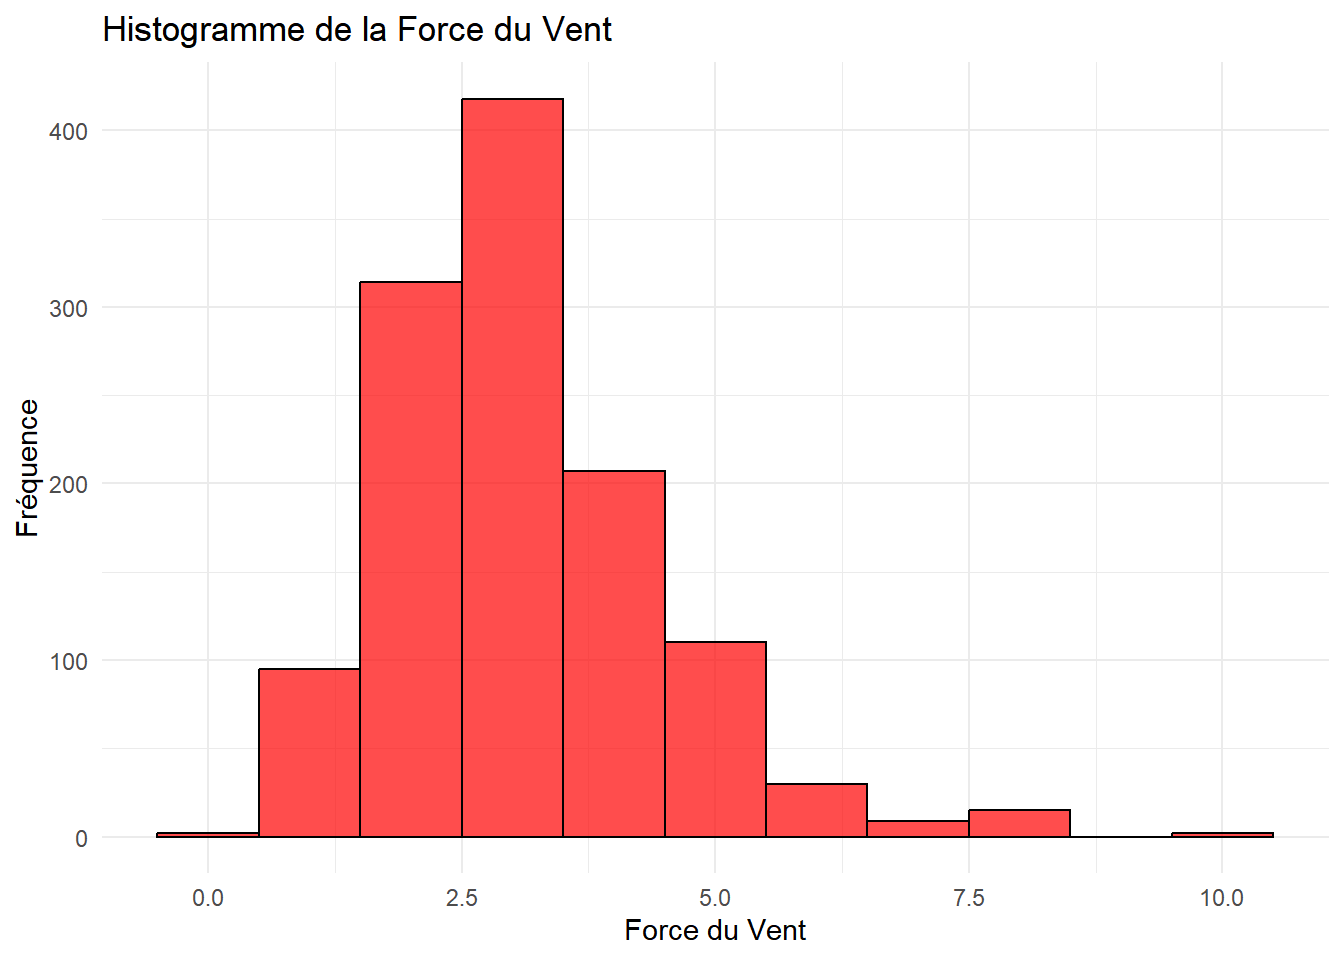
\includegraphics{Rapport_files/figure-latex/unnamed-chunk-8-1.pdf}

Dans ce graphique, nous avons tracé une courbe de densité pour illustrer
la répartition de la puissance du vent dans nos données.Ainsi, l'axe des
X reflète la force du vent tandis que l'axe des Y indique la densité,
c'est-à-dire en d'autres termes,la fréquence relative plutôt que le
nombre absolu.

La densité sert à normaliser l'histogramme afin qu'il présente une
surface totale de 1, ce qui simplifie la comparaison entre différentes
distributions ayant des échantillons variés.

La courbe de densité représente une estimation non paramétrique de la
fonction de densité des probabilités. Elle est fluide et représente la
probabilité que les observations prennent une valeur dans une certaine
plage de force du vent.

La courbe de densité fournit une indication sur la structure globale de
la distribution des données.

Si la courbe est centrée sur une certaine valeur, cela signifie que la
plupart des données sont groupées autour de cette valeur.

Si la courbe est plate ou étendue, cela suggère une plus grande
variabilité des données.

Nous allons également décrire la manière dont nous avons réalisé la
partie informatique en utilisant la fonction
\textbf{geom\_histogram(aes(y = ..density..))}, ce qui nous a permis de
construire l'histogramme. L'argument \textbf{aes(y = ..density..)}
spécifie que l'axe des ordonnées doit refléter la densité plutôt que la
fréquence brute. Cela nous permettra de standardiser les données afin
que l'aire totale sous l'histogramme soit de 1.

La commande \textbf{geom\_density(color = ``blue'', size = 1)} nous
offre la possibilité d'intégrer la courbe de densité.

La fonction \textbf{labs(title = ``Distribution de la Force du Vent avec
Courbe de Densité'', x = ``Force du Vent'', y = ``Densité'')} nous donne
la possibilité de spécifier le titre du diagramme ainsi que les
étiquettes des axes X et Y.

La fonction \textbf{theme\_minimal()} applique un style épuré au
graphique, éliminant les éléments visuels superflus.

\begin{enumerate}
\def\labelenumi{\arabic{enumi}.}
\setcounter{enumi}{1}
\tightlist
\item
  \textbf{Surface parcourue par le feu en fonction de la force du vent}
\end{enumerate}

\begin{Shaded}
\begin{Highlighting}[]
\FunctionTok{library}\NormalTok{(ggplot2)}

\NormalTok{data }\OtherTok{\textless{}{-}} \FunctionTok{read.csv}\NormalTok{(}\StringTok{"../Exports/export\_vents.csv"}\NormalTok{)}

\FunctionTok{ggplot}\NormalTok{(data, }\FunctionTok{aes}\NormalTok{(}\AttributeTok{x =}\NormalTok{ Force\_vent\_med, }\AttributeTok{y =}\NormalTok{ surface\_parcourue\_m2)) }\SpecialCharTok{+}
  \FunctionTok{geom\_point}\NormalTok{(}\AttributeTok{color =} \StringTok{"black"}\NormalTok{, }\AttributeTok{size =} \DecValTok{2}\NormalTok{) }\SpecialCharTok{+} 
  \FunctionTok{labs}\NormalTok{(}\AttributeTok{title =} \StringTok{"Surface Parcourue par le Feu en fonction de la Force du Vent"}\NormalTok{, }
       \AttributeTok{x =} \StringTok{"Force du Vent"}\NormalTok{, }
       \AttributeTok{y =} \StringTok{"Surface Parcourue (m²)"}\NormalTok{) }\SpecialCharTok{+}
  \FunctionTok{theme\_minimal}\NormalTok{() }\SpecialCharTok{+}  \CommentTok{\# Thème minimal pour une présentation épurée}
  \FunctionTok{theme}\NormalTok{(}
    \AttributeTok{axis.text.x =} \FunctionTok{element\_text}\NormalTok{(}\AttributeTok{angle =} \DecValTok{45}\NormalTok{, }\AttributeTok{hjust =} \DecValTok{1}\NormalTok{),}
    \AttributeTok{axis.text.y =} \FunctionTok{element\_text}\NormalTok{(}\AttributeTok{size =} \DecValTok{12}\NormalTok{),}
    \AttributeTok{axis.title =} \FunctionTok{element\_text}\NormalTok{(}\AttributeTok{size =} \DecValTok{14}\NormalTok{, }\AttributeTok{face =} \StringTok{"bold"}\NormalTok{),}
    \AttributeTok{plot.title =} \FunctionTok{element\_text}\NormalTok{(}\AttributeTok{size =} \DecValTok{16}\NormalTok{, }\AttributeTok{face =} \StringTok{"bold"}\NormalTok{, }\AttributeTok{hjust =} \FloatTok{0.5}\NormalTok{)}
\NormalTok{  )}
\end{Highlighting}
\end{Shaded}

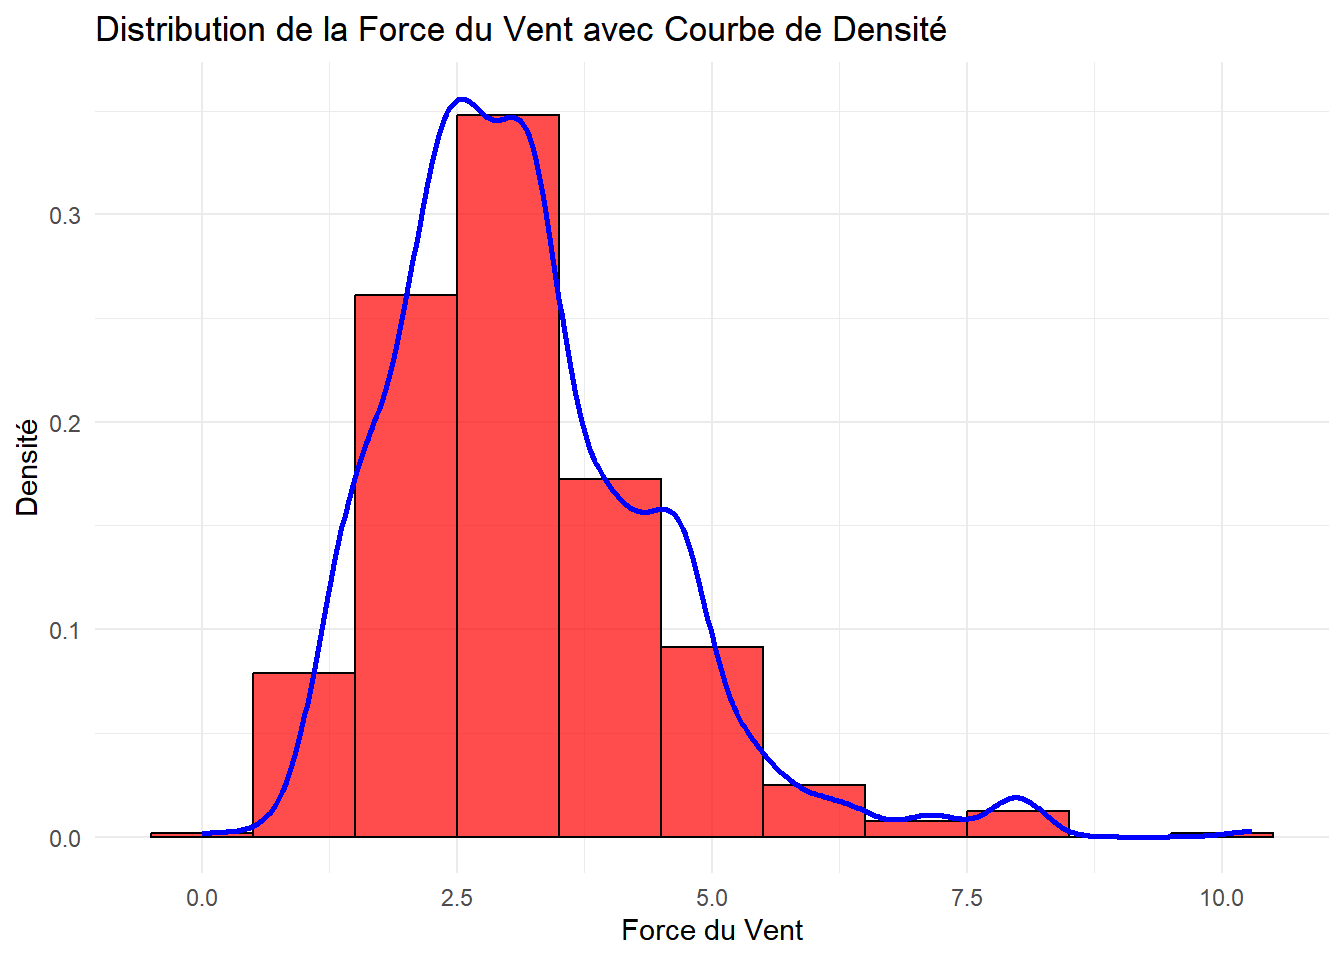
\includegraphics{Rapport_files/figure-latex/unnamed-chunk-9-1.pdf}

\begin{enumerate}
\def\labelenumi{\arabic{enumi}.}
\tightlist
\item
  \textbf{Analyse Informatique:}
\end{enumerate}

Tout d'abord, nous allons décrire comment nous avons développé notre
code. Pour commencer, nous avons importé notre bibliothèque ggplot2 afin
de créer des visualisations complexes en langage R. Par la suite, nous
avons chargé notre fichier contenant les données grâce à la méthode
\textbf{read.csv()} et avons assigné le résultat à une variable nommée
data. Cette variable data représente l'objet où nous conservons ces
informations.

Ensuite, nous élaborons notre diagramme de dispersion en utilisant la
méthode \textbf{ggplot()}, qui intègre les données. Par ailleurs, l'axe
des x, déterminé par l'aes, représentera la force du vent alors que
l'axe des y illustrera la surface parcourue en m².

Actuellement, nous sommes dans la phase où nous ajoutons des points pour
pouvoir représenter les données. Nous utilisons la méthode
\textbf{geom\_point()} pour ce faire. Nous avons spécifié la couleur des
points en noir et aussi déterminé la taille des points pour une
visibilité optimale en utilisant l'option size = 2.

Pour une lecture optimale du graphique, nous avons utilisé la fonction
\textbf{labs()}. Nous avons ajouté le titre au graphique et précisé les
noms des deux axes en recourant à x et y.

Comme le graphe precedent on a utilise la methode du
\textbf{theme\_minimal()} pour le mettre dans un desin plus minimaliste

À l'instar du graphique précédent, nous avons employé la technique du
\textbf{theme\_minimal()} afin de le présenter dans une design plus
épuré.

Pour accroître la clarté des axes et du titre, nous faisons appel à la
fonction \textbf{theme()}. En manipulant \textbf{axis.text.x} et
\textbf{axis.text.y}, nous avons employé l'option \textbf{element\_text}
pour le rendre incliné, modifier sa taille, etc. Quant aux attributs des
deux axes, nous avons utilisé axis.title pour mettre le texte en gras
grâce à l'attribut \textbf{face}.Pour le titre principal du graphique,
on utilise \textbf{plot.title} pour ajuster ses caractéristiques à
l'aide de \textbf{size}, \textbf{face} et \textbf{hjust}.L'utilisation
de \textbf{hjust} permet de positionner le titre au centre.

\begin{enumerate}
\def\labelenumi{\arabic{enumi}.}
\setcounter{enumi}{1}
\tightlist
\item
  \textbf{Analyse Statistique:}
\end{enumerate}

Commençons par examiner ce sous-problème qui se focalise sur la
superficie que couvre le feu en relation avec l'intensité du vent. Tout
d'abord, on remarque que la force du vent varie entre 0 et 10 unités. De
plus, la superficie affectée par le feu ou les incendies est presque de
0 à 1 000 000.

On remarque une concentration significative de points entre 0 et 5
unités de force du vent, avec une superficie allant de 0 à environ 750
000 m².

Il est également possible de conclure qu'au-delà de cinq unités, les
points commencent à devenir rares et la surface parcourue tend à se
stabiliser tout en réduisant légèrement.

L'accumulation de points indique qu'une intensification du vent a
tendance à élargir la portée du feu, particulièrement dans le cas de
vents faibles à modérés.Toutefois, ce lien n'est pas rigoureusement
linéaire, étant donné la large répartition des points.

Au-delà d'une certaine intensité de vent (approximativement 7-8 unités),
la surface couverte ne paraît pas s'accroître de manière
proportionnelle, ce qui pourrait suggérer un phénomène de saturation ou
des éléments restrictifs (tels que la disponibilité du combustible,
l'humidité ou la topographie).

Il est également important de souligner que la puissance du vent joue un
rôle crucial dans la diffusion des incendies, puisqu'elle transporte de
l'oxygène et les particules embrasées amplifient ainsi la vitesse de
propagation et l'étendue touchée. Ceci justifie l'orientation initiale à
la hausse.

\textbf{Synthese de la Problematique}

Ainsi, pour résumer cette question, nous avons d'abord établi une
corrélation entre la force du vent et la superficie touchée par le
feu.Nous avons constaté qu'il n'y a pas de relation linéaire entre ces
deux facteurs. Pour saisir plus fidèlement la complexité de la relation,
nous avons réalisé une régression polynomiale de degré 2. Cette méthode
nous a autorisé à noter que la surface affectée par l'incendie a
tendance à croître plus significativement à des niveaux faibles de la
force du vent avant de diminuer à mesure que cette dernière devient plus
intense.Cela indique qu'il y a une dynamique non linéaire entre ces deux
éléments,avec un effet d'accélération initial suivi d'un processus de
plafonnement.

L'analyse effectuée sur l'histogramme et la courbe de densité a montré
que la majorité des forces du vent se concentre autour de valeurs basses
à modérées, avec une queue notable vers les valeurs plus hautes.Cela
indique que, dans notre échantillon,les vents de faible à moyenne
intensité sont prédominants, tandis que les vents de très haute
intensité sont plutôt rares.

Le diagramme de dispersion a révélé une tendance à l'augmentation de la
superficie brûlée avec la puissance du vent, bien que cette corrélation
ne soit pas entièrement linéaire. Les informations suggèrent que, face à
des vents de faible à modéré (jusqu'à environ 5 unités de force),la
superficie touchée par le feu s'accroît rapidement.Toutefois, au-delà
d'un certain seuil de force du vent, l'expansion de la zone parcourue
semble se stabiliser, indiquant d'autres facteurs limitants que'il ne
s'agit pas seulement du vent, comme la disponibilité du carburant ou la
configuration du terrain.

Les données recueillies indiquent que même si la puissance du vent a un
impact significatif sur l'expansion des incendies, elle ne constitue pas
le seul élément décisif.D'autres facteurs tels que la disponibilité des
carburants, l'humidité du sol et la topographie locale ont aussi un
impact sur la diffusion du feu.Ainsi, même si une augmentation de la
vitesse du vent peut effectivement favoriser la diffusion des incendies,
cette corrélation devient moins directe et plus complexe lorsque le vent
atteint des intensités plus extrêmes.

\subparagraph{4.3.2.4 Impact des conditions météorologiques extrêmes sur
les
incendies}\label{impact-des-conditions-muxe9tuxe9orologiques-extruxeames-sur-les-incendies}

\subparagraph{4.3.2.5 Effet des radiations solaires sur les
incendies}\label{effet-des-radiations-solaires-sur-les-incendies}

\subparagraph{4.3.2.6 Température et nombre d'incendies par période de
la
journée}\label{tempuxe9rature-et-nombre-dincendies-par-puxe9riode-de-la-journuxe9e}

\subparagraph{4.3.2.7 Relation entre la force du vent et la propagation
des
incendies}\label{relation-entre-la-force-du-vent-et-la-propagation-des-incendies}

\subparagraph{4.3.2.8 Impact de la pression de vapeur sur la vitesse de
propagation des
incendies}\label{impact-de-la-pression-de-vapeur-sur-la-vitesse-de-propagation-des-incendies}

\paragraph{4.3.3 Géographie et
environnement}\label{guxe9ographie-et-environnement}

\subparagraph{4.3.3.1 Propagation des incendies sur le territoire
Francais}\label{propagation-des-incendies-sur-le-territoire-francais}

\begin{Shaded}
\begin{Highlighting}[]
\ImportTok{import}\NormalTok{ geopandas }\ImportTok{as}\NormalTok{ gpd}
\ImportTok{import}\NormalTok{ pandas }\ImportTok{as}\NormalTok{ pd}
\ImportTok{import}\NormalTok{ matplotlib.pyplot }\ImportTok{as}\NormalTok{ plt}

\NormalTok{df }\OperatorTok{=}\NormalTok{ pd.read\_csv(}\StringTok{"../Data/donnees\_geo.csv"}\NormalTok{)}

\NormalTok{chemin\_fichier\_geojson }\OperatorTok{=} \StringTok{"../Data/contour{-}des{-}departements.geojson"}  
\NormalTok{gdf\_departements }\OperatorTok{=}\NormalTok{ gpd.read\_file(chemin\_fichier\_geojson)}

\NormalTok{fig, ax }\OperatorTok{=}\NormalTok{ plt.subplots(figsize}\OperatorTok{=}\NormalTok{(}\DecValTok{15}\NormalTok{, }\DecValTok{15}\NormalTok{))  }

\NormalTok{gdf\_departements.plot(ax}\OperatorTok{=}\NormalTok{ax, color}\OperatorTok{=}\StringTok{"lightgray"}\NormalTok{, edgecolor}\OperatorTok{=}\StringTok{"black"}\NormalTok{)}

\NormalTok{ax.scatter(df[}\StringTok{"longitude"}\NormalTok{], df[}\StringTok{"latitude"}\NormalTok{], color}\OperatorTok{=}\StringTok{"red"}\NormalTok{, s}\OperatorTok{=}\DecValTok{50}\NormalTok{, label}\OperatorTok{=}\StringTok{"Incendies"}\NormalTok{)  }


\NormalTok{ax.set\_xlim([ }\OperatorTok{{-}}\FloatTok{5.5}\NormalTok{, }\DecValTok{10}\NormalTok{ ])}
\end{Highlighting}
\end{Shaded}

\begin{verbatim}
## (-5.5, 10.0)
\end{verbatim}

\begin{Shaded}
\begin{Highlighting}[]
\NormalTok{ax.set\_ylim([}\FloatTok{41.5}\NormalTok{, }\FloatTok{51.5}\NormalTok{])   }
\end{Highlighting}
\end{Shaded}

\begin{verbatim}
## (41.5, 51.5)
\end{verbatim}

\begin{Shaded}
\begin{Highlighting}[]
\NormalTok{plt.title(}\StringTok{"Carte des Incendies par Département"}\NormalTok{, fontsize}\OperatorTok{=}\DecValTok{20}\NormalTok{)}
\NormalTok{plt.legend()}

\NormalTok{ax.set\_axis\_off()}

\NormalTok{plt.savefig(}\StringTok{"carte\_incendies\_departements\_geojson\_grande\_avec\_points\_agrandis.png"}\NormalTok{, dpi}\OperatorTok{=}\DecValTok{600}\NormalTok{, bbox\_inches}\OperatorTok{=}\StringTok{\textquotesingle{}tight\textquotesingle{}}\NormalTok{)}

\NormalTok{plt.show()}
\end{Highlighting}
\end{Shaded}

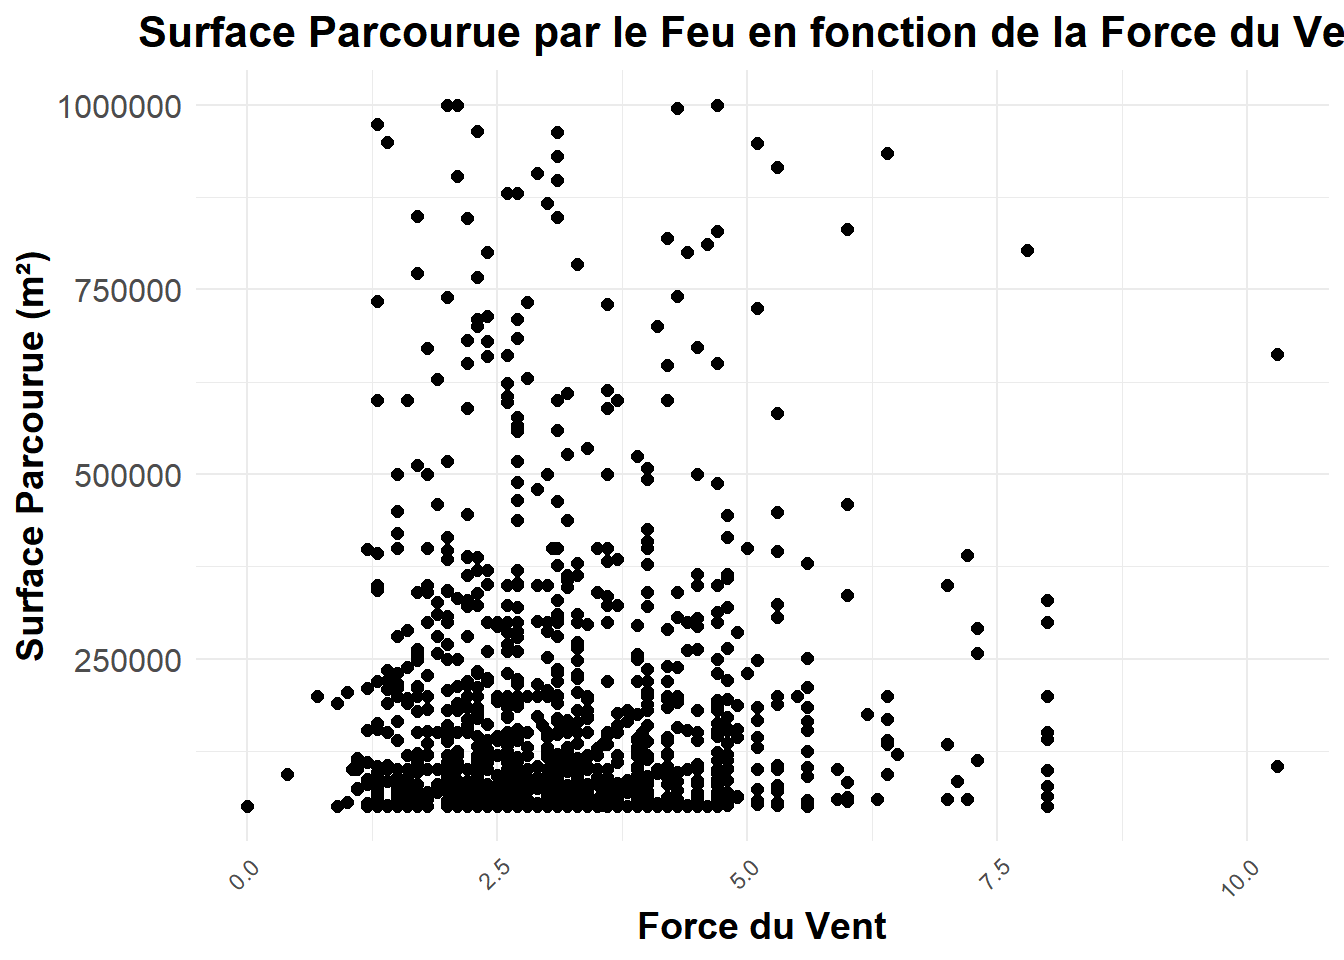
\includegraphics{Rapport_files/figure-latex/unnamed-chunk-10-1.pdf}

Nous allons examiner l'analyse de la propagation des incendies à travers
le territoire français après avoir utilisé ces informations sur la carte
nationale de France.

Décomposons la France, qui est reconnue comme un État composé de
régions. Ces régions sont elles-mêmes constituées de sous-régions, qui à
leur tour regroupent des départements, et ces derniers, des communes.

En France, on compte 13 régions spécifiquement dans la partie
métropolitaine. Nous allons d'abord les nommer, puis commencer leur
énumération et enfin procéder à leur analyse.

\begin{enumerate}
\def\labelenumi{\arabic{enumi}.}
\tightlist
\item
  Auvergne-Rhône-Alpes
\item
  Bourgogne-Franche-Comté
\item
  Bretagne
\item
  Centre-Val de Loire
\item
  Corse
\item
  Grand Est
\item
  Hauts-de-France
\item
  Île-de-France
\item
  Normandie
\item
  Nouvelle-Aquitaine
\item
  Occitanie
\item
  Pays de la Loire
\item
  Provence-Alpes-Côte d'Azur
\end{enumerate}

Nous procéderons à l'examen de ces 13 régions individuellement, pour
finalement en arriver à une conclusion.

La région \textbf{Auvergne Rhône-Alpes} présente un taux d'incendies
relativement bas, l'une des raisons étant qu'elle jouit d'un climat plus
diversifié que celui d'autres régions du sud.Cette région a des
altitudes plus élevées qui entraînent une température plus fraîche et un
climat plus humide, ce qui diminue le danger d'incendies de grande
envergure.

Le climat tempéré de la région \textbf{Bourgogne Franche Comté},
caractérisé par des hivers rigoureux et des étés modérés, explique son
taux d'incendies inférieur comparativement à la région Auvergne
Rhône-Alpes. Cette région abrite des montagnes et des collines comme le
Jura et les Vosges, qui sont habituellement plus humides et moins
prédisposées aux incendies forestiers. De plus, cette zone est surtout
composée de forêts de feuillus (chênes, hêtres, érables) et de prairies
qui présentent une moindre inflammabilité par rapport aux résineux ou
aux maquis méditerranéens.

La région de \textbf{Bretagne}, en raison de son climat océanique et de
ses températures modérées tout au long de l'année, présente un taux
réduit d'incendies.Les hivers sont tempérés et les étés restent frais,
accompagnés d'une humidité importante. En outre, les précipitations
régulières et l'humidité persistante durant toute l'année préservent la
végétation plus verdoyante et moins aride, contribuant ainsi à réduire
le danger d'incendies.

Il y a effectivement certains incendies dans la région
\textbf{Centre-Val de Loire}.Cette région jouit d'un climat continental,
caractérisé par des hivers rigoureux et des étés plus tempérés en
comparaison avec les régions du sud de la France. La région se compose
de plaines et de collines, ce qui réduit la probabilité d'incidents
majeurs et fait baisser le taux d'incendies dans le centre du Val de
Loire.

\textbf{La Corse} est une des zones sensibles aux incendies en raison de
divers éléments géographiques, climatiques, etc.La Corse jouit d'un
climat méditerranéen marqué par des étés extrêmement chauds et arides,
ce qui favorise l'apparition aisée d'incendies.Les températures
estivales peuvent atteindre des sommets extrêmes, créant un
environnement propice à la diffusion rapide des incendies. Cette zone
peut être exposée à des rafales puissantes comme le Mistral qui
facilitent la diffusion des feux.Ces courants d'air puissants et
généralement secs peuvent propulser les flammes sur de vastes étendues,
compliquant ainsi l'éradication des incendies.

La région \textbf{Grand-est} présente une moindre susceptibilité aux
incidents, mais elle n'est pas totalement épargnée.Cette région jouit
d'un climat diversifié qui subit des influences à la fois océaniques et
continentales.Les hivers sont rigoureux, les étés sont torrides,
cependant ils ne parviennent pas à égaler ceux du sud de la France en
termes de températures.L'incidence des périodes de sécheresse est en
baisse, diminuant ainsi le danger des incendies. En outre, cette région
est dotée de magnifiques zones montagneuses et de vastes plaines. Cette
région bénéficie d'une pluviométrie plutôt stable, surtout en automne et
en février. Ces précipitations contribuent à conserver un certain degré
d'humidité dans le sol et la végétation, ce qui diminue les risques
d'incendies.

Le climat humide, la présence de forêts de feuillus, le relief plat et
les vents modérés contribuent à rendre la région des
\textbf{Hauts-de-France} relativement moins vulnérable aux
incendies.Ainsi, les conditions météorologiques et géographiques sont
généralement moins favorables aux incendies sévères que d'autres zones
situées au sud.

\textbf{L'Île-de-France}, étant la région où se trouve la
\textbf{capitale}, est la plus densément peuplée et urbanisée de France.
Elle est moins sujette aux grands incendies que les régions situées au
sud du pays. En revanche, cette région n'est pas entièrement protégée
contre les incendies. Cette région jouit d'un climat océanique tempéré
caractérisé par des hivers rigoureux et des étés doux. En outre, la
topographie de l'Ile-de-France est principalement plane ou légèrement
vallonnée, en contraste avec les régions montagneuses telles que les
Alpes ou les Pyrénées.

La région de \textbf{Normandie} affiche un taux réduit d'incendies.Grace
à son climat océanique tempéré, son niveau de précipitations constant,
sa topographie relativement plane et sa végétation essentiellement
feuillue, la Normandie est moins sujette aux incendies que d'autres
zones en France.Ces facteurs contribuent à une augmentation de
l'humidité dans l'environnement, réduisant par conséquent le risque
d'incendies. Néanmoins, des incendies sporadiques peuvent encore
survenir, principalement dans les régions boisées et rurales pendant les
périodes de sécheresse ou de chaleur intense, même s'ils restent
relativement peu fréquents par rapport aux zones plus chaudes et sèches
du pays.

La région \textbf{Nouvelle Aquitaine}, située dans le sud-ouest, est
susceptible de subir des incendies, notamment à cause de son climat et
de sa végétation. Cette région présente un climat plutôt océanique à
l'ouest et méditerranéen à l'est, ce qui signifie que les étés peuvent
être particulièrement chauds et secs, surtout dans les zones limitrophes
de l'Espagne et du Pays Basque. Par ailleurs, les vagues de chaleur
peuvent entraîner des phases d'aridité prolongées qui créent un
environnement propice aux incendies.

\textbf{L'Occitanie} est une des régions les plus vulnérables aux
incendies en raison de divers facteurs géographiques, climatiques et
écologiques.Dans sa partie méridionale et sud, cette région jouit d'un
climat méditerranéen avec des étés chauds et secs.Durant l'été, les
températures peuvent grimper à des sommets élevés et la région est
susceptible de connaître des phases d'aridité prolongées, des
circonstances propices aux incendies. Dans la propagation des incendies,
le vent, notamment le Mistral et la Tramontane qui balaye
occasionnellement la zone, a un impact crucial.

La région du \textbf{Pays de la Loire} présente une exposition moindre
aux incendies par rapport à d'autres régions. Le climat de cette zone
est océanique, c'est-à-dire qu'il offre des hivers doux et des étés
tempérés, avec des précipitations régulières tout au long de l'année.
Les vagues de chaleur se produisent généralement dans d'autres zones,
comme le sud-est de la France, ce qui rend la région moins susceptible
aux incendies liés à la canicule.

Pour conclure, la dernière région est la \textbf{Provence Alpes Côte
d'Azur}, qui se trouve dans le sud-est et subit une forte influence de
divers facteurs climatiques et géographiques.Cette région jouit d'un
climat méditerranéen, marqué par des étés très chauds et secs ainsi que
des hivers doux et humides. Durant l'été, les températures peuvent
atteindre des niveaux extrêmement élevés avec des vagues de chaleur qui
se produisent fréquemment. On peut également observer que cette zone est
celle où le taux d'incendies est le plus élevé.

Suite à l'étude de la progression du taux d'incendies sur la carte
nationale que nous avons réalisée, il est évident que la région où le
taux d'incendies est le plus élevé est la \textbf{Côte d'Azur}. En
revanche, les zones où le taux d'incendies est le plus faible incluent
des régions telles que les \textbf{Pays de la Loire},
\textbf{Normandie}, etc. Il est donc clair que les conditions
météorologiques et la localisation géographique de la ville ou de la
région ont un impact crucial, surtout lorsque les conditions climatiques
sont particulièrement propices aux incendies. De même, la nature des
forêts situées dans les zones urbaines a une incidence significative sur
l'expansion des feux.Bien qu'il existe une différence de taux
d'incendies entre la ville et la montagne, cette question sera examinée
dans le cadre d'une autre problèmatique.

\subparagraph{4.3.3.2 Comparaison de la fréquence des incendies dans les
régions montagneuses vs basses
altitudes}\label{comparaison-de-la-fruxe9quence-des-incendies-dans-les-ruxe9gions-montagneuses-vs-basses-altitudes}

L'objectif de cette étude est d'examiner et de comparer le lien entre
les incendies et l'altitude dans diverses régions et départements en
France.

Les données utilisées sont issues de deux sources majeures. Un fichier
CSV contient divers attributs, parmi lesquels nous avons choisi ceux qui
nous intéressent, à savoir les données concernant la superficie des
terrains brûlés, la nature de ces feux, ainsi qu'un fichier géographique
comprenant des renseignements sur l'altitude moyenne de chaque
municipalité.

Cette analyse vise à déterminer si les incidents ont tendance à être
plus fréquents ou plus graves aux altitudes élevées comparativement aux
altitudes inférieures.

\textbf{Avant de procéder à l'analyse, nous allons décrire nos données.}

Les informations sur les incendies incluent des données concernant la
superficie des incendies exprimées en \textbf{surface\_parcourue\_m2},
ainsi que le type d'incendie principal et secondaire indiqué soit par
\textbf{nature\_inc\_prim}, soit par \textbf{nature\_inc\_sec}. De plus,
nous disposons de détails chronologiques tels que \textbf{année, mois,
jour, heure}.

Le fichier \textbf{donnes\_geo} nous donne des renseignements sur la
hauteur moyenne de chaque commune, illustrée en \textbf{altitude\_med},
ce qui nous aidera à catégoriser les incendies selon leur altitude en
deux options : soit \textbf{haute}, soit \textbf{basse} altitude.

Dans cette analyse cruciale, nous avons utilisé une variable
catégorielle \textbf{altitude\_zone} qui classe chaque commune selon son
altitude moyenne : soit en zones de \textbf{basse altitude} en utilisant
une délimitation de \textbf{moins de 1000 mètres} que nous avons
employée pour les altitudes inférieures, soit en zones de \textbf{haute
altitude} grâce à une dénomination \textbf{au-dessus de 1000 mètres.}

Apres avoir decrits touts els donnees qu'on possede pour cette anaylyse
on va commencer a calculer la \textbf{correlation de Pearson}. On va
calculer la correlation entre la surface des incendies et l'altitude. Le
but de cella la est de voir si il existe \textbf{une relation lineaire}
entre la surface des incendies et l'altitude.

On va y calculer la correlation et apres on va analyser le graphe de la
correlation de Pearson

\begin{Shaded}
\begin{Highlighting}[]
\NormalTok{incendiesregions }\OtherTok{\textless{}{-}} \FunctionTok{read.csv}\NormalTok{(}\StringTok{"../Exports/export\_incendiesregions.csv"}\NormalTok{)}
\NormalTok{correlation }\OtherTok{\textless{}{-}} \FunctionTok{cor}\NormalTok{(incendiesregions}\SpecialCharTok{$}\NormalTok{surface\_parcourue\_m2, incendiesregions}\SpecialCharTok{$}\NormalTok{altitude\_med, }\AttributeTok{use =} \StringTok{"complete.obs"}\NormalTok{)}

\FunctionTok{print}\NormalTok{(}\FunctionTok{paste}\NormalTok{(}\StringTok{"Corrélation de Pearson entre la surface des incendies et l\textquotesingle{}altitude : "}\NormalTok{, }\FunctionTok{round}\NormalTok{(correlation, }\DecValTok{2}\NormalTok{)))}
\end{Highlighting}
\end{Shaded}

\begin{verbatim}
## [1] "Corrélation de Pearson entre la surface des incendies et l'altitude :  0"
\end{verbatim}

Nous observons une corrélation de 0, ce qui indique qu'il n'y a pas de
lien linéaire entre les deux variables. Nous concluons donc qu'elles
sont indépendantes l'une de l'autre.

\begin{Shaded}
\begin{Highlighting}[]
\NormalTok{incendiesregions }\OtherTok{\textless{}{-}} \FunctionTok{read.csv}\NormalTok{(}\StringTok{"../Exports/export\_incendiesregions.csv"}\NormalTok{)}
\FunctionTok{ggplot}\NormalTok{(incendiesregions, }\FunctionTok{aes}\NormalTok{(}\AttributeTok{x =}\NormalTok{ altitude\_med, }\AttributeTok{y =}\NormalTok{ surface\_parcourue\_m2)) }\SpecialCharTok{+}
  \FunctionTok{geom\_point}\NormalTok{(}\AttributeTok{color =} \StringTok{"blue"}\NormalTok{, }\AttributeTok{alpha =} \FloatTok{0.6}\NormalTok{) }\SpecialCharTok{+}
  \FunctionTok{labs}\NormalTok{(}\AttributeTok{title =} \StringTok{"Corrélation entre l\textquotesingle{}altitude et la surface des incendies"}\NormalTok{,}
       \AttributeTok{x =} \StringTok{"Altitude (m)"}\NormalTok{, }\AttributeTok{y =} \StringTok{"Surface parcourue des incendies (m²)"}\NormalTok{) }\SpecialCharTok{+}
  \FunctionTok{theme\_minimal}\NormalTok{() }\SpecialCharTok{+}
  \FunctionTok{geom\_smooth}\NormalTok{(}\AttributeTok{method =} \StringTok{"lm"}\NormalTok{, }\AttributeTok{se =} \ConstantTok{FALSE}\NormalTok{, }\AttributeTok{color =} \StringTok{"red"}\NormalTok{)}
\end{Highlighting}
\end{Shaded}

\begin{verbatim}
## `geom_smooth()` using formula = 'y ~ x'
\end{verbatim}

\includegraphics{Rapport_files/figure-latex/unnamed-chunk-12-1.pdf}

1- \textbf{Analyse Informatique du Graphe de Corrélation }

On a commencé par charger le fichier CSV (valeurs séparées par des
virgules) en utilisant la méthode prédéfinie \textbf{read.csv}. Nous
avons également eu recours à la bibliothèque ggplot2 pour réaliser le
graphique qui sera ensuite soumis à une analyse statistique.

De plus, nous avons précisé dans la méthode \textbf{ggplot} le paramètre
contenant le fichier CSV ainsi que l'\textbf{aesthetics} d'où nous
indiquons les axes X et Y.

Par la suite, on utilise geom-point() pour intégrer des points
(\textbf{scatter plot}) au diagramme.Dans notre schéma, chaque duo
illustre une paire de valeurs.L'option color donne la faculté de changer
la couleur des points en bleu, tandis que l'option alpha permet de
définir leur degré de transparence.

Un \textbf{alpha} de 1 signifierait une opacité totale, alors qu'un
alpha de 0 indiquerait une transparence totale.

Par la suite, nous employons la fonction \textbf{labs()} pour attribuer
des étiquettes au graphique et nous intégrons la méthode
\textbf{theme\_minimal} afin d'appliquer un style contemporain à notre
diagramme.

Pour appliquer le graphique de corrélation, nous employons la méthode
\textbf{geom\_smooth()} qui nous donne l'opportunité d'intégrer la ligne
de tendance, également connue sous le nom de courbe de régression, sur
le graphique.Cela vise à mettre en évidence une tendance globale entre
les variables.

Nous aimerions faire un récapitulatif des options disponibles dans la
méthode geom\_smooth() :

\begin{itemize}
\item
  L'option \textbf{method = ``lm''} indique qu'une régression linéaire
  est employée. Cette régression va nous révéler le lien linéaire entre
  l'altitude et la superficie des feux de forêt.
\item
  L'option \textbf{se=FALSE} nous permet d'éviter l'affichage de
  l'intervalle de confiance.
\item
  L'option \textbf{color = ``red''} sert à définir la couleur de la
  courbe de régression en rouge.
\end{itemize}

2- \textbf{Analyse Statistique:}

En examinant notre diagramme de façon statistique, nous notons que l'Axe
des X illustrant l'altitude s'étend de 0 à 2000 mètres. Concernant l'axe
des Y, il indique la superficie des incendies allant de 0 à 1 000 000
m², même si la plupart des points se regroupent sous les 750 000 m².
Nous précisons que les points bleus sur notre graphique correspondent
aux observations individuelles de la superficie des incendies à diverses
altitudes.

On note une importante densité de points à des altitudes faibles
(proches du niveau de la mer), accompagnée d'une grande variabilité dans
la superficie des incendies, qui peut atteindre environ 750 000 m².
Quand l'altitude dépasse 500m, la quantité de points diminue et
l'étendue des incendies paraît généralement moins importante avec très
peu de cas où les feux excèdent 250,000 m2 au-delà de 1000m. La ligne
rouge horizontale, placée autour de 250,000 m², représente une référence
ou, pour dire autrement, la moyenne.

On observe une tendance à la baisse de la superficie des incendies
lorsque l'altitude augmente. On pourrait également affirmer que le taux
d'incendies en montagne sera inférieur à celui observé en milieu urbain.
Il est crucial de noter que l'écart entre les points est significatif,
surtout à basse altitude, ce qui suggère que le lien n'est pas fortement
linéaire. Cela peut être influencé par divers éléments tels que le
climat, la végétation, l'activité humaine, etc., qui pourraient affecter
l'étendue des incendies.

Une fois la corrélation de Pearson calculée, nous allons maintenant
procéder à la mise en œuvre d'une régression polynomiale, à condition
que nous admettions que les deux variables sont indépendantes
linéairement.

\begin{Shaded}
\begin{Highlighting}[]
\NormalTok{incendiesregions }\OtherTok{\textless{}{-}} \FunctionTok{read.csv}\NormalTok{(}\StringTok{"../Exports/export\_incendiesregions.csv"}\NormalTok{)}
\FunctionTok{ggplot}\NormalTok{(incendiesregions, }\FunctionTok{aes}\NormalTok{(}\AttributeTok{x =}\NormalTok{ altitude\_med, }\AttributeTok{y =}\NormalTok{ surface\_parcourue\_m2)) }\SpecialCharTok{+}
  \FunctionTok{geom\_point}\NormalTok{(}\AttributeTok{color =} \StringTok{"blue"}\NormalTok{, }\AttributeTok{alpha =} \FloatTok{0.6}\NormalTok{) }\SpecialCharTok{+}
  \FunctionTok{labs}\NormalTok{(}\AttributeTok{title =} \StringTok{"Régression Polynomiale entre Altitude et Surface des Incendies"}\NormalTok{,}
       \AttributeTok{x =} \StringTok{"Altitude (m)"}\NormalTok{, }\AttributeTok{y =} \StringTok{"Surface parcourue des incendies (m²)"}\NormalTok{) }\SpecialCharTok{+}
  \FunctionTok{theme\_minimal}\NormalTok{() }\SpecialCharTok{+}
  \FunctionTok{geom\_smooth}\NormalTok{(}\AttributeTok{method =} \StringTok{"lm"}\NormalTok{, }\AttributeTok{formula =}\NormalTok{ y }\SpecialCharTok{\textasciitilde{}} \FunctionTok{poly}\NormalTok{(x, }\DecValTok{2}\NormalTok{), }\AttributeTok{se =} \ConstantTok{FALSE}\NormalTok{, }\AttributeTok{color =} \StringTok{"red"}\NormalTok{)}
\end{Highlighting}
\end{Shaded}

\includegraphics{Rapport_files/figure-latex/unnamed-chunk-13-1.pdf}

\textbf{On va en premier analyser en premier une Analyse Informatique et
puis une Analyse Statistique:}

1- \textbf{Analyse Informatique:}

Nous utilisons également la bibliothèque \textbf{ggplot2} ici. Nous
commençons à construire notre graphique en invoquant la méthode
\textbf{ggplot()}, tout en précisant le DataFrame. En définissant
l'\textbf{aes}, nous déterminons les axes x et y. Ensuite, nous traçons
les points sur le graphique en spécifiant leurs couleurs et
transparences. Par la suite, nous ajoutons les étiquettes à notre
graphique et appliquons le \textbf{theme\_minimal()} afin de lui
conférer une apparence moderne.

On finit par tracer la courbe de la régression polynomiale en employant
la méthode \textbf{geom\_smooth()}. Il est précisé que la méthode
employée sera la régression linéaire, puis on note le score de la
formule de régression polynomiale en utilisant poly(x,2). On indique que
l'on souhaite x et x2, pas seulement x. \textbf{Se} implique que nous
masquons l'intervalle de confiance.

2- \textbf{Analyse Statistique:}

Nous allons examiner le graphique de la régression polynomiale entre
l'altitude et la superficie des feux de forêt. L'axe des x va de 0 à
2000 mètres, tandis que l'axe des y s'étend de 0 à 1 000 000 m², avec
une grande partie des points situés au-dessus de 750 000 m².

Les observations individuelles sont représentées (la superficie des
incendies à diverses altitudes).En outre, la ligne rouge qui entoure
environ 250,000 m² représente la régression polynomiale.

La régression des points correspond à l'analyse antérieure du graphique,
présentant une altitude basse de 0 à 500m avec une large variabilité
allant jusqu'à 750,000 m2. On observe une diminution graduelle de la
densité des points et des surfaces à mesure que l'altitude s'accroît.

La courbe de régression polynomiale est une ligne légèrement montante.

Après avoir effectué ces deux calculs, nous passerons à l'étape
d'analyse approfondie de nos données.Nous commencerons par examiner la
surface d'altitude par zone d'altitude.

\begin{enumerate}
\def\labelenumi{\arabic{enumi}.}
\tightlist
\item
  \textbf{L'analyse de la surface des incendies par zone d'altitude}
\end{enumerate}

Pour ce faire, nous allons construire notre histogramme puis réaliser
deux types d'analyses : une analyse informatique et une autre
statistique.

\begin{Shaded}
\begin{Highlighting}[]
\NormalTok{incendiesregions }\OtherTok{\textless{}{-}} \FunctionTok{read.csv}\NormalTok{(}\StringTok{"../Exports/export\_incendiesregions.csv"}\NormalTok{)}
\FunctionTok{ggplot}\NormalTok{(incendiesregions, }\FunctionTok{aes}\NormalTok{(}\AttributeTok{x =}\NormalTok{ surface\_parcourue\_m2, }\AttributeTok{fill =}\NormalTok{ altitude\_zone)) }\SpecialCharTok{+}
  \FunctionTok{geom\_histogram}\NormalTok{(}\AttributeTok{binwidth =} \DecValTok{5000}\NormalTok{, }\AttributeTok{position =} \StringTok{"dodge"}\NormalTok{, }\AttributeTok{alpha =} \FloatTok{0.7}\NormalTok{) }\SpecialCharTok{+}
  \FunctionTok{labs}\NormalTok{(}\AttributeTok{title =} \StringTok{"Distribution de la surface des incendies par zone d\textquotesingle{}altitude"}\NormalTok{,}
       \AttributeTok{x =} \StringTok{"Surface des incendies (m²)"}\NormalTok{, }\AttributeTok{y =} \StringTok{"Fréquence"}\NormalTok{) }\SpecialCharTok{+}
  \FunctionTok{theme\_minimal}\NormalTok{()}
\end{Highlighting}
\end{Shaded}

\includegraphics{Rapport_files/figure-latex/unnamed-chunk-14-1.pdf}

1- \textbf{Analyse Informatique:}

Pour dessiner cet histogramme, nous avons utilisé la bibliothèque
\textbf{ggplot2}.Dans un premier temps, nous avons importé les données
du fichier CSV dans une variable sous forme de DataFrame.

Par la suite, nous avons utilisé la méthode ggplot().Cette dernière
nécessite en paramètres la variable où les données sont entreposées
ainsi que l'aes où nous spécifions nos deux axes, x et y, le x
représentant ici la surface des incendies. Nous avons ensuite coloré les
barres de l'histogramme en fonction des différentes zones d'altitude.

Pour intégrer l'histogramme, nous avons utilisé la méthode
\textbf{geom\_histogram} qui nécessite plusieurs paramètres. Parmi ces
paramètres, nous indiquons la largeur des classes ou en d'autres termes,
le \textbf{binwidth}, qui sera fixé à 5000 m² pour agrégater les
incendies en segments de 5000 m². Nous spécifions également que les
barres seront disposées en mode \textbf{dodge}, c'est-à-dire côte à côte
pour chaque zone afin de faciliter la comparaison entre les différentes
catégories.Et finalement, nous précisons que la transparence des
couleurs sera de \textbf{0,7}, afin de simplifier l'interprétation de
notre histogramme.

Ensuite, nous intégrons le titre et les étiquettes à notre histogramme
en utilisant la méthode prédéfinie \textbf{labs()}. Cette dernière
nécessite deux paramètres : title pour attribuer un titre au graphique,
ainsi que x et y pour nommer respectivement les axes des abscisses et
des ordonnées.

Pour personnaliser le thème, nous avons employé la méthode prédéfinie
\textbf{theme\_minimal()} pour conférer un style contemporain.

2- \textbf{Analyse Statistique:}

Les incendies constituent un défi majeur pour la gestion des risques
liés à l'environnement, aux personnes et à la sécurité. Comprendre leur
distribution spatiale, en particulier par rapport à l'altitude, nous
aide à repérer les zones sensibles et à ajuster nos stratégies de
prévention.

Cette étude vise à examiner les informations fournies sur les surfaces
brouillées dans quatre zones d'altitude, allant de la basse à la haute
altitude.

Nous visons à identifier les tendances et à examiner leurs causes
potentielles.

La description des données mentionne quatre valeurs principales qui
correspondent aux zones brûlées.

La plupart des feux dans ces deux zones se situent sur des surfaces
plutôt réduites, allant de 0 à 250 000 m². Cela est signalé par les
fréquences élevées.

Alors que la superficie s'accroît au-delà de 250,000 m², le taux
d'incendies chute rapidement pour les deux zones, avec très peu d'entre
elles dépassant les 500,000 m².

Nous allons maintenant présenter la comparaison entre les deux
principales zones, Zone Basse et Zone Haute.

Nous allons débuter avec la Zone Basse. Cette région affiche une
occurrence nettement supérieure, en particulier pour les petites
surfaces, avec un sommet frôlant les 100.On peut donc supposer que les
incendies de petite à moyenne envergure se produisent beaucoup plus
souvent en zone basse.En d'autres termes,on peut constater que les
incendies surviennent plus souvent dans les villes ou les communes
situées à une altitude basse.

Concernant la région à altitude élevée.La survenue de ces incendies est
moins fréquente,avec des sommets pouvant aller jusqu'à 10 - 20 sur une
même étendue de terrain.

Cela suggère que les incendies sont moins courants dans les zones
élevées, ou que leur portée est plus restreinte.

Pour le dire autrement, on peut affirmer que la fréquence des incendies
est plus élevée dans les villes ou communes situées à une altitude
importante.

Suite à l'étude des deux régions en altitude, nous allons discuter de la
tendance globale.

La distribution présente une forme d'atténuation exponentielle que l'on
pourrait qualifier de queue lourde selon les statistiques, pour ces deux
zones.

On peut également affirmer que la probabilité de voir se produire des
incendies de grande ampleur dépassant les 500,000 m2 est extrêmement
faible.

Il est à noter que, au-delà de \textbf{750,000 m2}, les incendies d'une
très grande envergure sont peu fréquents dans ces deux régions.

Le mode en statistique, représentant la valeur la plus courante dans nos
données, est positionné sur la première barre pour les deux zones.
Cependant, son accentuation est davantage marquée en zone basse.

La variation des surfaces brûlées est plus significative dans les zones
où les incendies englobent une vaste étendue de terrain avec une
fréquence remarquée. Dans les zones élevées, la dispersion est moindre
avec une concentration autour des petites surfaces.

La distribution présente une forte asymétrie à droite (avec une biais
positif) et possède une longue queue pour les grandes superficies, même
si cette dernière est pratiquement nulle au-delà de 500,000 m2.

Il est probable que les incendies dans les zones basses soient plus
courants en raison des conditions environnementales propices (végétation
dense, températures élevées, accès humain facilité).

La fréquence des incendies en zones élevées pourrait être due à des
éléments tels qu'une végétation moins dense, un climat plus frais ou une
accessibilité restreinte.

L'occurrence rare de vastes incendies dépassant les 500,000 m2 dans ces
deux régions pourrait témoigner de mesures efficaces ou de barrières
naturelles (comme la topographie et l'humidité).

On pourrait finalement convenir que ce graphique indique une fréquence
et une variété nettement plus grandes des incendies en termes de
superficie dans les zones de basse altitude, avec une prédominance
marquée des petits incendies qui se propagent entre 0 et 250,000 m².

Dans les zones élevées, les incendies sont moins fréquents et se
restreignent généralement aux petites superficies.

\begin{enumerate}
\def\labelenumi{\arabic{enumi}.}
\setcounter{enumi}{1}
\tightlist
\item
  \textbf{La surface des incendies par zone haute et baisse des
  altitudes}
\end{enumerate}

Donc en premier on va dresser notre \textbf{boxplot}. On indique que le
boxplot il est utile pour pouvoir visualiser la repartition des donnees.

\begin{Shaded}
\begin{Highlighting}[]
\NormalTok{incendiesregions }\OtherTok{\textless{}{-}} \FunctionTok{read.csv}\NormalTok{(}\StringTok{"../Exports/export\_incendiesregions.csv"}\NormalTok{)}
\FunctionTok{ggplot}\NormalTok{(incendiesregions, }\FunctionTok{aes}\NormalTok{(}\AttributeTok{x =}\NormalTok{ altitude\_zone, }\AttributeTok{y =}\NormalTok{ surface\_parcourue\_m2)) }\SpecialCharTok{+}
  \FunctionTok{geom\_boxplot}\NormalTok{(}\AttributeTok{fill =} \FunctionTok{c}\NormalTok{(}\StringTok{"lightblue"}\NormalTok{, }\StringTok{"lightgreen"}\NormalTok{)) }\SpecialCharTok{+}
  \FunctionTok{labs}\NormalTok{(}\AttributeTok{title =} \StringTok{"Surface des incendies par zone d\textquotesingle{}altitude"}\NormalTok{, }
       \AttributeTok{x =} \StringTok{"Zone d\textquotesingle{}altitude"}\NormalTok{, }
       \AttributeTok{y =} \StringTok{"Surface parcourue (m²)"}\NormalTok{) }\SpecialCharTok{+}
  \FunctionTok{theme\_minimal}\NormalTok{()}
\end{Highlighting}
\end{Shaded}

\includegraphics{Rapport_files/figure-latex/unnamed-chunk-15-1.pdf}

1- \textbf{Analyse Informatique:}

D'abord, nous soulignons que ce diagramme en boîte, également connu sous
le nom de \textbf{boxplot} en anglais, nous donnera la possibilité
d'observer la répartition des surfaces brûlées dues à des feux dans deux
principales zones.

Comme à l'accoutumée, nous importons les données dans une variable sous
forme de DataFrame en spécifiant le chemin relatif du fichier contenant
ces données.

Par la suite, on utilise la méthode \textbf{ggplot} pour créer un
graphique initial à l'aide du package \textbf{ggplot2}.Ainsi, dans cette
approche, on recourt à la variable qui contient les données précédemment
stockées comme paramètre.Ensuite, nous définissons l'altitude comme
l'axe des x et nous alignons les ordonnées sur l'axe des y.

On précise que \textbf{altitude\_zone} fait référence aux catégories
d'altitudes, qu'elles soient basses ou élevées, et que
\textbf{surface\_parcourue\_m2} représente la superficie brûlée en
mètres carrés.

Pour intégrer le graphique dans le box, on emploie la méthode préétablie
de la bibliothèque \textbf{geom\_boxplot()}. qui va produire un boxplot,
une forme de représentation graphique qui permet d'illustrer la
dispersion des données, y compris la valeur médiane, etc. Par ailleurs,
l'option fill nous autorisera à spécifier les teintes pour remplir les
boutes.

On attribue finalement des titres et des étiquettes aux axes ainsi qu'au
graphique en utilisant la fonction prédéfinie \textbf{labs()}. Pour
personnaliser et moderniser le thème, comme à l'accoutumée, nous
utilisons la fonction prédéfinie \textbf{theme\_minimal}.

2- \textbf{Analyse Statistique}

Nous allons procéder à une analyse statistique de notre graphique qui
est illustré par un \textbf{diagramme en boîte}.Nous allons comparer la
répartition de la superficie des incendies exprimée en m² dans deux
régions d'altitude : basse et haute.

Nous débutons la présentation des composantes de notre graphique avec
l'axe Y, qui illustre la superficie parcourue en m² sur une échelle
allant de 0 à 1 000 000 m².L'axe X dépeint quant à lui les deux
catégories : Basse et Haute.

Notre graphique présente deux boîtes, chacune d'elles illustrant la
répartition des données avec des moustaches et des points qui
symbolisent les valeurs extrêmes. Il est à noter que la zone
\textbf{Basse} est indiquée en \textbf{bleu clair} et la zone
\textbf{Haute} en \textbf{vert pâle}.

Nous allons définir un \textbf{BoxPlot} comme contenant les informations
suivantes :

\begin{itemize}
\item
  La ligne médiane dans la boîte est un indicateur de la
  \textbf{Médiane}.
\item
  Les \textbf{Quartiles} sont les extrémités de la boîte qui illustrent
  le premier quartile.
\item
  Les \textbf{Moustaches} s'étendent habituellement jusqu'aux valeurs
  extrêmes, maximales et minimales.
\item
  Les \textbf{Points} symbolisent les valeurs extrêmes qui dépassent les
  moustaches.
\end{itemize}

La Zone Basse englobe la région médiatique où elle semble se déployer
sur environ 200,000 m2. Les moustaches de cette zone basse s'étendent
jusqu'à 50,000 m en profondeur et 500,000 m2 en hauteur.

De plus, on peut observer une multitude de points entre 500,000 et
1,000,000 qui signalent des incendies d'une ampleur exceptionnelle.

Concernant la Zone Haute, sa superficie s'étend approximativement de
100,000 m2 à 250,000 m2.

De plus, elle semble légèrement inférieure à celle de la Zone Basse qui
est d'environ 150,000 - 175,000 m2.

Les moustaches se déploient sur une superficie d'environ 50 000 m² en
bas et de 500 000 m² en haut.

On constate que moints de points abeerant que dans la Zone Basse avec
quelques valeurs entre 500,000 et 750,000 m2.

En observant les deux zones, on remarque :

\begin{itemize}
\item
  On constate que la \textbf{mediane} est supérieure dans la
  \textbf{Zone Basse}, avoisinant les 200,000 m2, par rapport à la zone
  Haute, où elle se situe entre 150,000 et 175,000 m2. Cela indique que
  les incendies ont tendance à occuper une superficie plus importante en
  altitude inférieure.
\item
  Les deux boîtes sont asymétriques du côté droit.
\item
  La Zone Basse présente davantage de valeurs extrêmes jusqu'à 1,000,000
  m2 comparativement à la Zone Haute qui atteint jusqu'à 750,000 m2.
  Cela pourrait indiquer que les conditions sont propices à des
  incendies hors du commun en basse altitude.
\end{itemize}

Il est possible que les incendies plus importants en basse altitude
soient attribuables à une abondance accrue de combustible (forêts
denses, broussailles) ou à une facilité d'accès pour des facteurs
humains (déclenchements de feu).

À haute altitude, les conditions plus sévères pourraient entraver la
propagation.

Il est possible de déduire à partir de cette sous-problématique que ce
graphique illustre une disparité dans l'étendue des incendies en
fonction de l'altitude.

Les régions de basse altitude présentent une superficie parcourue
nettement plus grande que les zones situées en haute altitude.

Cette variation est biologiquement justifiée par l'augmentation de la
densité de végétation combustibles, une intervention humaine plus
prononcée ou même des conditions météorologiques plus favorables au
déclenchement d'incendies dans les zones basses.

3- \textbf{La variation de la surface des incendies au fils des années:}

\begin{Shaded}
\begin{Highlighting}[]
\NormalTok{incendiesregions }\OtherTok{\textless{}{-}} \FunctionTok{read.csv}\NormalTok{(}\StringTok{"../Exports/export\_incendiesregions.csv"}\NormalTok{)}
\FunctionTok{ggplot}\NormalTok{(incendiesregions, }\FunctionTok{aes}\NormalTok{(}\AttributeTok{x =}\NormalTok{ annee, }\AttributeTok{y =}\NormalTok{ surface\_parcourue\_m2, }\AttributeTok{color =}\NormalTok{ altitude\_zone)) }\SpecialCharTok{+}
  \FunctionTok{geom\_line}\NormalTok{() }\SpecialCharTok{+}
  \FunctionTok{labs}\NormalTok{(}\AttributeTok{title =} \StringTok{"Variation de la surface des incendies au fil des années"}\NormalTok{,}
       \AttributeTok{x =} \StringTok{"Année"}\NormalTok{, }\AttributeTok{y =} \StringTok{"Surface parcourue des incendies (m²)"}\NormalTok{) }\SpecialCharTok{+}
  \FunctionTok{theme\_minimal}\NormalTok{()}
\end{Highlighting}
\end{Shaded}

\includegraphics{Rapport_files/figure-latex/unnamed-chunk-16-1.pdf}

1- \textbf{Analyse Informatique:}

Nous commencerons par réaliser une analyse informatique en détaillant la
façon dont nous avons programmé ce graphique, puis nous passerons à
l'analyse scientifique.

Dans un premier temps, nous avons assigné les données sous forme de
tableau DataFrame à une variable qui utilise la méthode prédéfinie
\textbf{read.csv} pour permettre la lecture des données.

Par la suite, nous avons créé le graphique en utilisant la méthode
ggplot, qui prend deux arguments majeurs :la variable contenant les
données et l'aes aesthetics qui va représenter les axes x et y.

De plus, il est précisé que chaque zone d'altitude sera illustrée par
une couleur distincte.

Par la suite, une ligne est dessinée pour relier les points de données
correspondant à chaque zone d'altitude.

Nous précisons que chaque courbe indique une altitude distincte, ce qui
nous permet d'examiner la progression des incendies en fonction des
années et de l'altitude.

Pour accomplir cela, nous avons utilisé la méthode \textbf{geom-line()}.

Pour personnaliser notre graphique, nous allons attribuer des noms aux
étiquettes et aux titres en utilisant la méthode prédéfinie
\textbf{labs()}.

De plus, afin d'appliquer un thème moderne de style épuré à chaque
graphique, nous utilisons la méthode \textbf{theme\_minimal()}.

2- \textbf{Analyse Statistique:}

Ce graphique présente une série temporelle avec des divisions annuelles
sur l'axe horizontal (X) couvrant la période de 2012 à 2023, et
représente la superficie affectée par les incendies en mètres carrés sur
l'axe vertical (Y), allant de 0 à 1 million de m².

Les données que nous détenons sont présentées sous forme de tracés en
zigzag avec des segments verticaux, ce qui nous permet de supposer qu'il
s'agit de lignes accompagnées d'intervalles de confiance.

Deux zones en altitude y sont présentes.\\
La région supérieure, illustrée en cyan, représente les zones brûlées à
\textbf{haute altitude}, tandis que la zone inférieure, signalée en
rouge, dénote les surfaces incendiées à \textbf{basse altitude.}

Chaque point sur la ligne représente une \textbf{estimation annuelle},
tandis que les segments verticaux illustrent une \textbf{variabilité}.

\textbf{Par rapport à la zone Basse :}

\begin{itemize}
\item
  \textbf{De 2012 à 2014}, la superficie couverte reste assez limitée,
  oscillant autour de 100 000 m² avec des sommets avoisinant à peu près
  250 000 m².Les segments verticaux montrent une \textbf{variabilité
  modérée}, avec des sommets avoisinant les 500,000 m² en 2013.
\item
  \textbf{Entre 2015 et 2017}, on a observé une hausse notable avec des
  valeurs moyennes avoisinant les 200,000 m². Cependant, des sommets
  extrêmes ont été atteints, notamment à 1,000,000 m² en 2016 et 2017.
  Cela nous conduit à interpréter qu'il y a eu des incendies d'une
  \textbf{ampleur exceptionnelle.}
\item
  \textbf{De 2018 à 2020}, la superficie moyenne connaît une légère
  baisse oscillant entre 50,000 et 150,000 m². Cependant, les segments
  verticaux continuent à afficher des pics élevés (jusqu'à 800,000 m² en
  2019). Au cours de cette période, la variabilité demeure
  significative.
\item
  \textbf{De 2021 à 2023}, on observe une tendance générale à la
  diminution, avec des moyennes se situant autour de 50 000 m².
  Cependant, les pics récurrents aux alentours de 500 000 - 750 000 m²
  démontrent que ces incendies extrêmes continuent de se produire.
\end{itemize}

\textbf{Pour ce qui est de la Zone Haute :}

\begin{itemize}
\item
  \textbf{De 2012 à 2014}, les zones ravagées par le feu sont
  généralement très petites, rarement supérieures à 50 000 m², avec des
  pics ne dépassant pas 100 000 m². On en conclut que la fluctuation
  entre 2012 et 2014 est restreinte.
\item
  On remarque une hausse abrupte entre \textbf{2015 et 2016}, culminant
  en 2016 avec une moyenne d'environ 300 000 m2 et un record proche de
  750 000 m2. Cela suggère qu'un phénomène atypique a eu lieu en haute
  altitude.
\item
  \textbf{De 2017 à 2020}, suite à ce pic, les superficies retombent à
  des niveaux faibles, que l'on peut estimer à une moyenne de 50 000 m².
  Des pics occasionnels peuvent atteindre environ 500 000 m² en 2019.
\item
  \textbf{De 2021 à 2023}, la tendance demeure constante avec des
  superficies moyennes faibles avoisinant les 50 000 m² et des pics plus
  modestes atteignant jusqu'à 250 000 m², suggérant une diminution des
  incendies extrêmes en haute altitude.
\end{itemize}

Les deux zones montrent une grande variabilité d'année en année, mais on
remarque que la Zone Basse affiche constamment des superficies brûlées
plus importantes et des extrêmes plus prononcés que la Zone Haute.

Cela confirme l'interprétation du diagramme en boîte précédent, où les
incendies en altitude basse étaient plus répandus et plus variables.

On observe une correspondance entre les deux régions, particulièrement
aux alentours de 2016-2017 où les deux présentent des pics.

On peut en déduire que cela découle de facteurs climatiques et
environnementaux partagés.

Les segments verticaux s'étendent bien plus haut que bas, ce qui nous
autorise à conclure qu'il s'agit d'une distribution asymétrique vers la
droite.

La concordance des deux zones, approximativement entre 2016 et
2017,pourrait être attribuée à des conditions météorologiques telles
qu'une sécheresse prolongée ou des températures élevées qui facilitent
la diffusion des incendies.

La région basse présentant systématiquement des superficies plus
étendues est vulnérable à ces circonstances en raison d'une densité de
végétation plus importante ou d'une accessibilité humaine accrue.

La Zone Haute présente généralement des zones brûlées plus réduites,
sans doute en raison de conditions moins propices à la propagation
telles que la présence réduite de combustible, des températures plus
fraîches et des sols rocailleux.

Cependant, le record de 2016 indique que des phénomènes rares comme les
vents violents ou les éclairs peuvent causer des incendies conséquents
même à haute altitude.

Concernant les tendances récentes, la baisse des zones incendiées après
2020 dans les deux régions pourrait témoigner d'initiatives de
prévention telles que la gestion forestière,la lutte anti-incendie ou
encore des modifications climatiques comme une augmentation de la
fréquence des précipitations. 4- \textbf{Les Catégories des Incendies
par zone d'altitude:}

\begin{Shaded}
\begin{Highlighting}[]
\NormalTok{incendiesregions }\OtherTok{\textless{}{-}} \FunctionTok{read.csv}\NormalTok{(}\StringTok{"../Exports/export\_incendiesregions.csv"}\NormalTok{)}
\FunctionTok{ggplot}\NormalTok{(incendiesregions, }\FunctionTok{aes}\NormalTok{(}\AttributeTok{x =}\NormalTok{ altitude\_zone, }\AttributeTok{fill =}\NormalTok{ nature\_inc\_prim)) }\SpecialCharTok{+}
  \FunctionTok{geom\_bar}\NormalTok{(}\AttributeTok{position =} \StringTok{"stack"}\NormalTok{) }\SpecialCharTok{+}
  \FunctionTok{labs}\NormalTok{(}\AttributeTok{title =} \StringTok{"Repartition des types d\textquotesingle{}incendies par zone d\textquotesingle{}altitude"}\NormalTok{,}
       \AttributeTok{x =} \StringTok{"Zone d\textquotesingle{}altitude"}\NormalTok{, }\AttributeTok{y =} \StringTok{"Nombre d\textquotesingle{}incendies"}\NormalTok{) }\SpecialCharTok{+}
  \FunctionTok{theme\_minimal}\NormalTok{()}
\end{Highlighting}
\end{Shaded}

\includegraphics{Rapport_files/figure-latex/unnamed-chunk-17-1.pdf}

1- \textbf{Analyse Informatique:}

On a d'abord chargé les données dans une variable qui contient les
données sous la forme d'un tableau dataframe provenant du fichier CSV
contenant toutes les informations requises.

Par la suite, on emploie la méthode \textbf{gplot} qui est prédéfinie
dans la bibliothèque \textbf{ggplot2}. Pour générer le graphique basé
sur les informations du fichier CSV, elle nécessite deux paramètres clés
: le premier est la variable qui contient les données et l'autre est
l'\textbf{aes aesthetics} où l'on spécifie l'axe des x qui illustrera
les différentes zones d'altitude. Nous activons également l'option
\textbf{fill} pour permettre une coloration en fonction du type
d'incendie indiqué dans la variable **nature\_inc-\_prim**.

Ensuite, nous ajoutons les barres empilées au graphique en utilisant la
méthode prédéfinie \textbf{geom\_bar}. Nous précisons que la position
sera \textbf{stack}, ce qui signifie que les barres seront superposées
et chaque couleur représentera une catégorie distincte de
\textbf{nature\_insc\_prim}. La hauteur totale de la barre indiquera le
nombre total d'incendies dans chaque zone d'altitude.

Si l'on souhaite se baser sur la proportion des différents types
d'incendies plutôt que sur les valeurs absolues, on pourrait recourir à
la valeur \textbf{fill}. Cela nous aidera à normaliser les barres afin
qu'elles aient toutes la même hauteur, illustrant ainsi la proportion de
chaque type d'incendie.

\textbf{Nous allons insérer le graphique joint, cependant, nous ne
procéderons pas à l'analyse de la position fill, mais plutôt à celle de
la position stack}

\begin{Shaded}
\begin{Highlighting}[]
\NormalTok{incendiesregions }\OtherTok{\textless{}{-}} \FunctionTok{read.csv}\NormalTok{(}\StringTok{"../Exports/export\_incendiesregions.csv"}\NormalTok{)}
\FunctionTok{ggplot}\NormalTok{(incendiesregions, }\FunctionTok{aes}\NormalTok{(}\AttributeTok{x =}\NormalTok{ altitude\_zone, }\AttributeTok{fill =}\NormalTok{ nature\_inc\_prim)) }\SpecialCharTok{+}
  \FunctionTok{geom\_bar}\NormalTok{(}\AttributeTok{position =} \StringTok{"fill"}\NormalTok{) }\SpecialCharTok{+}
  \FunctionTok{labs}\NormalTok{(}\AttributeTok{title =} \StringTok{"Repartition des types d\textquotesingle{}incendies par zone d\textquotesingle{}altitude"}\NormalTok{,}
       \AttributeTok{x =} \StringTok{"Zone d\textquotesingle{}altitude"}\NormalTok{, }\AttributeTok{y =} \StringTok{"Nombre d\textquotesingle{}incendies"}\NormalTok{) }\SpecialCharTok{+}
  \FunctionTok{theme\_minimal}\NormalTok{()}
\end{Highlighting}
\end{Shaded}

\includegraphics{Rapport_files/figure-latex/unnamed-chunk-18-1.pdf}

Par la suite, nous intégrons les étiquettes et le titre en employant la
méthode prédéfinie \textbf{labs()}, en précisant les deux axes x et y
ainsi que le titre principal de notre graphique.

Et finalement, pour l'application d'un thème moderne au style épuré,
nous utilisons la méthode prédéfinie \textbf{theme\_minimal()}.

2- \textbf{Analyse Statistique:}

En guise d'introduction, voici un histogramme empilé qui illustre le
total des incendies dans deux zones distinctes, Basse et Haute.

Dans cette étude, on considère que la basse altitude est inférieure à
1000 mètres et la haute altitude, supérieure à 1000 mètres.

L'axe horizontal (X) illustre les zones d'altitudes, tandis que l'axe
vertical (Y) représente le nombre d'incendies, allant approximativement
de 0 à 1200.

Pour les types d'incendies, nous avons quatre catégories : accidentel
représenté en rouge, involontaire en vert, malveillance en cyan et
naturel en violet.

\textbf{Dans la Zone Basse la repartittion est estimee en :}

On fait une estimation d'environ \textbf{1200 incendies} dans \textbf{la
région basse}.

\begin{itemize}
\item
  \textbf{Maveillance} représente la plus grande proportion, soit
  environ \textbf{40 à 45\%}, ce qui équivaut approximativement à
  \textbf{500 incidents}.
\item
  Environ \textbf{30 à 50\%} des incendies, soit approximativement
  \textbf{400}, sont d'origine \textbf{involontaire}.
\item
  De manière \textbf{accidentelle}, environ \textbf{15 à 20 \%}, soit
  approximativement \textbf{200 incendies}.
\item
  \textbf{Naturelle} pas très faible, environ \textbf{5\%}, soit
  approximativement \textbf{50 incendies}.
\end{itemize}

\textbf{Dans la Zone Basse, on estime la répartition à : }

On estime que le nombre d'incendies dans la Zone \textbf{Haute} se situe
entre \textbf{150 et 200}.

\begin{itemize}
\item
  La \textbf{majorité}, soit environ \textbf{50\%}, représente
  approximativement entre \textbf{80 et 100 incendies involontaires. }
\item
  \textbf{Maveillance} dénote environ \textbf{30\%} de près de
  \textbf{50} incendies.
\item
  Environ \textbf{15\%} des incendies sont approximativement dus à une
  \textbf{négligence} ou un accident, soit environ \textbf{25} cas.
\item
  Environ \textbf{5\%} de la partie \textbf{naturelle} correspondent
  approximativement à une \textbf{dizaine d'incendies}.
\end{itemize}

Pour déterminer si la distribution des types d'incendies est influencée
par l'altitude de la zone, nous ferons appel au test d'indépendance du
Chi2.

Ce tableau a été élaboré sur la base d'estimations des données.

\begin{longtable}[]{@{}llll@{}}
\toprule\noalign{}
\textbf{Type d'incendie} & \textbf{Basse} & \textbf{Haute} &
\textbf{Total} \\
\midrule\noalign{}
\endhead
\bottomrule\noalign{}
\endlastfoot
Accidentelle & 200 & 30 & 230 \\
Involontaire & 400 & 100 & 500 \\
Malveillance & 500 & 50 & 550 \\
Naturelle & 50 & 10 & 60 \\
\textbf{Total} & 1200 & 200 & 1400 \\
\end{longtable}

On établit l'\textbf{Hypothèse Nulle (H0)} selon laquelle la
distribution des types d'incendies est indépendante de la zone
d'altitude.

\textbf{Hypothèse Alternative (H1)}La distribution est influencée par la
zone d'altitude.

Nous allons effectuer le calcul en employant le langage R.

\begin{Shaded}
\begin{Highlighting}[]
\NormalTok{observed }\OtherTok{\textless{}{-}} \FunctionTok{matrix}\NormalTok{(}\FunctionTok{c}\NormalTok{(}\DecValTok{200}\NormalTok{, }\DecValTok{400}\NormalTok{, }\DecValTok{500}\NormalTok{, }\DecValTok{50}\NormalTok{,  }\CommentTok{\# Zone Basse}
                     \DecValTok{30}\NormalTok{, }\DecValTok{100}\NormalTok{, }\DecValTok{50}\NormalTok{, }\DecValTok{10}\NormalTok{),   }\CommentTok{\# Zone Haute}
                   \AttributeTok{nrow =} \DecValTok{4}\NormalTok{, }\AttributeTok{byrow =} \ConstantTok{FALSE}\NormalTok{)}
\FunctionTok{rownames}\NormalTok{(observed) }\OtherTok{\textless{}{-}} \FunctionTok{c}\NormalTok{(}\StringTok{"Accidentelle"}\NormalTok{, }\StringTok{"Involontaire"}\NormalTok{, }\StringTok{"Malveillance"}\NormalTok{, }\StringTok{"Naturelle"}\NormalTok{)}
\FunctionTok{colnames}\NormalTok{(observed) }\OtherTok{\textless{}{-}} \FunctionTok{c}\NormalTok{(}\StringTok{"Basse"}\NormalTok{, }\StringTok{"Haute"}\NormalTok{)}

\FunctionTok{print}\NormalTok{(}\StringTok{"Fréquences observées :"}\NormalTok{)}
\end{Highlighting}
\end{Shaded}

\begin{verbatim}
## [1] "Fréquences observées :"
\end{verbatim}

\begin{Shaded}
\begin{Highlighting}[]
\FunctionTok{print}\NormalTok{(observed)}
\end{Highlighting}
\end{Shaded}

\begin{verbatim}
##              Basse Haute
## Accidentelle   200    30
## Involontaire   400   100
## Malveillance   500    50
## Naturelle       50    10
\end{verbatim}

\begin{Shaded}
\begin{Highlighting}[]
\NormalTok{row\_totals }\OtherTok{\textless{}{-}} \FunctionTok{rowSums}\NormalTok{(observed)}
\NormalTok{col\_totals }\OtherTok{\textless{}{-}} \FunctionTok{colSums}\NormalTok{(observed)}
\NormalTok{grand\_total }\OtherTok{\textless{}{-}} \FunctionTok{sum}\NormalTok{(observed)}

\NormalTok{expected }\OtherTok{\textless{}{-}} \FunctionTok{matrix}\NormalTok{(}\DecValTok{0}\NormalTok{, }\AttributeTok{nrow =} \DecValTok{4}\NormalTok{, }\AttributeTok{ncol =} \DecValTok{2}\NormalTok{)}
\ControlFlowTok{for}\NormalTok{ (i }\ControlFlowTok{in} \DecValTok{1}\SpecialCharTok{:}\DecValTok{4}\NormalTok{) \{}
  \ControlFlowTok{for}\NormalTok{ (j }\ControlFlowTok{in} \DecValTok{1}\SpecialCharTok{:}\DecValTok{2}\NormalTok{) \{}
\NormalTok{    expected[i, j] }\OtherTok{\textless{}{-}}\NormalTok{ (row\_totals[i] }\SpecialCharTok{*}\NormalTok{ col\_totals[j]) }\SpecialCharTok{/}\NormalTok{ grand\_total}
\NormalTok{  \}}
\NormalTok{\}}
\FunctionTok{rownames}\NormalTok{(expected) }\OtherTok{\textless{}{-}} \FunctionTok{rownames}\NormalTok{(observed)}
\FunctionTok{colnames}\NormalTok{(expected) }\OtherTok{\textless{}{-}} \FunctionTok{colnames}\NormalTok{(observed)}

\FunctionTok{print}\NormalTok{(}\StringTok{"Fréquences attendues :"}\NormalTok{)}
\end{Highlighting}
\end{Shaded}

\begin{verbatim}
## [1] "Fréquences attendues :"
\end{verbatim}

\begin{Shaded}
\begin{Highlighting}[]
\FunctionTok{print}\NormalTok{(}\FunctionTok{round}\NormalTok{(expected, }\DecValTok{2}\NormalTok{))}
\end{Highlighting}
\end{Shaded}

\begin{verbatim}
##               Basse Haute
## Accidentelle 197.39 32.61
## Involontaire 429.10 70.90
## Malveillance 472.01 77.99
## Naturelle     51.49  8.51
\end{verbatim}

\begin{Shaded}
\begin{Highlighting}[]
\NormalTok{chi2\_contrib }\OtherTok{\textless{}{-}} \FunctionTok{matrix}\NormalTok{(}\DecValTok{0}\NormalTok{, }\AttributeTok{nrow =} \DecValTok{4}\NormalTok{, }\AttributeTok{ncol =} \DecValTok{2}\NormalTok{)}
\ControlFlowTok{for}\NormalTok{ (i }\ControlFlowTok{in} \DecValTok{1}\SpecialCharTok{:}\DecValTok{4}\NormalTok{) \{}
  \ControlFlowTok{for}\NormalTok{ (j }\ControlFlowTok{in} \DecValTok{1}\SpecialCharTok{:}\DecValTok{2}\NormalTok{) \{}
\NormalTok{    chi2\_contrib[i, j] }\OtherTok{\textless{}{-}}\NormalTok{ (observed[i, j] }\SpecialCharTok{{-}}\NormalTok{ expected[i, j])}\SpecialCharTok{\^{}}\DecValTok{2} \SpecialCharTok{/}\NormalTok{ expected[i, j]}
\NormalTok{  \}}
\NormalTok{\}}
\NormalTok{chi2\_stat }\OtherTok{\textless{}{-}} \FunctionTok{sum}\NormalTok{(chi2\_contrib)}

\FunctionTok{print}\NormalTok{(}\StringTok{"Contributions au Chi² :"}\NormalTok{)}
\end{Highlighting}
\end{Shaded}

\begin{verbatim}
## [1] "Contributions au Chi² :"
\end{verbatim}

\begin{Shaded}
\begin{Highlighting}[]
\FunctionTok{print}\NormalTok{(}\FunctionTok{round}\NormalTok{(chi2\_contrib, }\DecValTok{4}\NormalTok{))}
\end{Highlighting}
\end{Shaded}

\begin{verbatim}
##        [,1]    [,2]
## [1,] 0.0346  0.2092
## [2,] 1.9740 11.9482
## [3,] 1.6592 10.0425
## [4,] 0.0433  0.2618
\end{verbatim}

\begin{Shaded}
\begin{Highlighting}[]
\FunctionTok{print}\NormalTok{(}\StringTok{"Statistique Chi² :"}\NormalTok{)}
\end{Highlighting}
\end{Shaded}

\begin{verbatim}
## [1] "Statistique Chi² :"
\end{verbatim}

\begin{Shaded}
\begin{Highlighting}[]
\FunctionTok{print}\NormalTok{(chi2\_stat)}
\end{Highlighting}
\end{Shaded}

\begin{verbatim}
## [1] 26.17275
\end{verbatim}

\begin{Shaded}
\begin{Highlighting}[]
\NormalTok{df }\OtherTok{\textless{}{-}}\NormalTok{ (}\FunctionTok{nrow}\NormalTok{(observed) }\SpecialCharTok{{-}} \DecValTok{1}\NormalTok{) }\SpecialCharTok{*}\NormalTok{ (}\FunctionTok{ncol}\NormalTok{(observed) }\SpecialCharTok{{-}} \DecValTok{1}\NormalTok{)}
\FunctionTok{print}\NormalTok{(}\StringTok{"Degré de liberté :"}\NormalTok{)}
\end{Highlighting}
\end{Shaded}

\begin{verbatim}
## [1] "Degré de liberté :"
\end{verbatim}

\begin{Shaded}
\begin{Highlighting}[]
\FunctionTok{print}\NormalTok{(df)}
\end{Highlighting}
\end{Shaded}

\begin{verbatim}
## [1] 3
\end{verbatim}

\begin{Shaded}
\begin{Highlighting}[]
\NormalTok{critical\_value }\OtherTok{\textless{}{-}} \FunctionTok{qchisq}\NormalTok{(}\FloatTok{0.95}\NormalTok{, df)}
\FunctionTok{print}\NormalTok{(}\StringTok{"Valeur critique (alpha = 0.05) :"}\NormalTok{)}
\end{Highlighting}
\end{Shaded}

\begin{verbatim}
## [1] "Valeur critique (alpha = 0.05) :"
\end{verbatim}

\begin{Shaded}
\begin{Highlighting}[]
\FunctionTok{print}\NormalTok{(critical\_value)}
\end{Highlighting}
\end{Shaded}

\begin{verbatim}
## [1] 7.814728
\end{verbatim}

La statistique du \(\chi^2\) calculée est \textbf{26.03}, avec \textbf{3
degrés de liberté} \((4-1) \times (2-1) = 3\).\\
À un seuil de signification \(\alpha = 0.05\), la valeur critique est
\textbf{7.815}.

Puisque la statistique observée \(26.03\) dépasse la valeur critique
\(7.815\), nous \textbf{rejetons l'hypothèse nulle} \(H_0\),\\
ce qui indique que la répartition des types d'incendies \textbf{dépend
de la zone d'altitude}.

On en déduit que les \textbf{plus grandes contributions} à la
statistique du \(\chi^2\) proviennent des catégories suivantes :

\begin{itemize}
\item
  \textbf{Involontaire (Zone Haute) -- 11.43 :}\\
  → Les incendies involontaires sont \textbf{surreprésentés} en haute
  altitude par rapport aux attentes sous \(H_0\).
\item
  \textbf{Malveillance (Zone Haute) -- 10.39 :}\\
  → Les incendies de malveillance sont \textbf{sous-représentés} en
  haute altitude.
\item
  \textbf{Involontaire (Zone Basse) -- 1.90} et \textbf{Malveillance
  (Zone Basse) -- 1.73 :}\\
  → Ces deux catégories contribuent également, mais de manière
  \textbf{moins marquée}.
\end{itemize}

Finalement, le test du Chi2 indique une corrélation notable entre la
sorte d'incendie et la zone d'altitude. Dans les zones à faible
altitude, la majorité des incendies sont dus à des actes de malveillance
(500 cas observés comparés à 471.73 attendus),tandis que dans les zones
en hauteur,il y a une surreprésentation des incendies accidentels (100
cas observés contre 71.43 attendus).

Ces observations indiquent que les éléments humains tels que les actes
malveillants en basse altitude et l'imprudence en haute altitude
contribuent de manière significative à la distribution des incendies, en
raison des disparités d'accessibilité, de densité démographique et
d'activités humaines entre les régions.

Dans une zone de faible altitude La prévalence des incendies d'actes de
malveillance à 41,67\% et involontaires à 33,33\% indique une influence
humaine significative.

Ceci est associé à une densité de population plus élevée, des activités
agricoles ou des actes criminels tels que les incendies volontaires.

Le faible pourcentage d'incendies naturels, soit 4.17\%, souligne que
les conditions naturelles ont une influence marginale.

Dans la Zone Haute, la prévalence des incendies accidentels à 50\%
pourrait témoigner d'actions humaines occasionnelles, tandis que la
proportion plus faible d'actes de malveillance à 25\% indique une
difficulté d'accès pour les actes délibérés.

Le taux d'incendies naturels demeure bas, s'établissant à 5\%, ce qui
est cohérent avec les altitudes élevées où les orages sont moins
fréquents ou moins enclins à provoquer des incendies.

L'analyse comparative des deux zones suggère que la
\textbf{surreprésentation des incendies de malveillance en basse
altitude}\\
pourrait être liée à des facteurs \textbf{sociaux et économiques}, tels
que :

\begin{itemize}
\tightlist
\item
  \textbf{Conflits locaux} ou \textbf{vandalisme},\\
\item
  \textbf{Activités agricoles}, notamment le \textbf{défrichement
  illégal}.
\end{itemize}

À l'inverse, en haute altitude, la \textbf{prédominance des incendies
involontaires} peut refléter des \textbf{erreurs humaines},\\
souvent associées à des activités comme les \textbf{loisirs en plein
air} ou des \textbf{travaux occasionnels}.

5- \textbf{Les Catégories des Incendies au fils des années:}

\begin{Shaded}
\begin{Highlighting}[]
\NormalTok{incendiesregions }\OtherTok{\textless{}{-}} \FunctionTok{read.csv}\NormalTok{(}\StringTok{"../Exports/export\_incendiesregions.csv"}\NormalTok{)}
\FunctionTok{ggplot}\NormalTok{(incendiesregions, }\FunctionTok{aes}\NormalTok{(}\AttributeTok{x =}\NormalTok{ annee, }\AttributeTok{fill =}\NormalTok{ nature\_inc\_prim)) }\SpecialCharTok{+}
  \FunctionTok{geom\_bar}\NormalTok{(}\AttributeTok{position =} \StringTok{"fill"}\NormalTok{) }\SpecialCharTok{+}  
  \FunctionTok{labs}\NormalTok{(}\AttributeTok{title =} \StringTok{"Repartition des types d\textquotesingle{}incendies par annee"}\NormalTok{,}
       \AttributeTok{x =} \StringTok{"Annee"}\NormalTok{,}
       \AttributeTok{y =} \StringTok{"Proportion"}\NormalTok{,}
       \AttributeTok{fill =} \StringTok{"Type d\textquotesingle{}incendie"}\NormalTok{) }\SpecialCharTok{+}
  \FunctionTok{theme\_minimal}\NormalTok{() }\SpecialCharTok{+}  
  \FunctionTok{scale\_fill\_brewer}\NormalTok{(}\AttributeTok{palette =} \StringTok{"Set2"}\NormalTok{)}
\end{Highlighting}
\end{Shaded}

\includegraphics{Rapport_files/figure-latex/unnamed-chunk-20-1.pdf}

1- \textbf{Analyse Informatique:}

Pour en pouvoir creer ce graphe on a en premier charger les donnees dans
une variable en utilisant la methode \textbf{read.csv} en specifiant en
parametre le chemin relatif du fichier CSV

Apres cela en utilisant la methode \textbf{gpplot()} en indiqyant dans
cette methode deux parametres principals la variables contenant la
donneeee sous format de DataFrame et l'aes aesthetics n specifiant l'axe
des x qui sera represente en anneee et on specifie que la barre des
graphes seront remplies par \textbf{nature\_inc\_prim} en specifiant le
type des incendies.

Apres cela en utilisant la methode predefine \textbf{geom\_bar()} en
mettant en parametre la position fill pour pouvoir normaliser les
hauteurs de barres pour que chaque barre represente une proportion et
non une valeur absolue.

Chaque barre est donc echeloneee de 0 a 1 ou chaque couleur qui est
remplie par \textbf{nature\_inc\_prim} represente une proportion au
total.

Pour pouvoir personaliser notre graphique en utilisant la methode
predefinie \textbf{labs()} on specifie le titre principale de notre
graphe et le titre des deux axes x et y respectivement , afin de rendre
le theme de notre graphe plus coherent et plus moderne on tuilise la
methode predefinei \textbf{theme\_minimal()}.

On utilise la methode predefinie \textbf{scale\_fill\_brewer()} pour
appliquer une pqlette de couleurs pre-definies par
\textbf{RColorBrewer}.La palette \textbf{Set2} est utilise pour permet
de colorier differentes categories de \textbf{nature\_inc\_prim} de
maniere distincte.

2- \textbf{Analyse Statistique:}

Dans ce diagramme, nous procéderons à une analyse statistique de notre
graphique.

Tout d'abord, on précise que l'axe des X couvre la période de
\textbf{2012 à 2023} avec une \textbf{échelle continue} et des
intervalles d'à peu près \textbf{0,5 an}. Quant à l'axe des Y, il est
illustré par le ratio des incendies allant de \textbf{0 à 1 (100\%)}.

\textbf{Il existe quatre catégories d'incendies :}

\begin{itemize}
\item
  Représenté par \textbf{Vert Clai}r, les incendies sont causés par des
  \textbf{accidents}.
\item
  \textbf{Involontaires} sont représentés par des incendies causés par
  des \textbf{négligence}s ou des facteurs \textbf{non intentionnels}.
\item
  \textbf{Malveillance} dépeinte par \textbf{Bleu} incendies
  \textbf{volontaires}.
\item
  \textbf{Rose} représente les incendies provoqués par des
  \textbf{phénomènes naturels}.
\end{itemize}

Il est à noter que chaque histogramme annuel illustre la répartition
proportionnelle des types d'incendies, avec une somme de ces proportions
pour chaque année qui s'élève toujours à 1, soit 100\%.

\textbf{Nous allons examiner de façon descriptive les tendances dans le
temps.}

\begin{itemize}
\item
  \textbf{Acte malveillant} :Cette catégorie prédomine presque tout au
  long de la période, avec des proportions variant entre 40 et 60\%, un
  sommet remarquable vers \textbf{2015-2016} où la proportion s'approche
  d'environ \textbf{60\%}. On a constaté une \textbf{légère baisse}
  après 2020, atteignant environ \textbf{40 \%} en \textbf{2022-2023}.
\item
  \textbf{Involontaire}:Durant la période, on observe une proportion
  notable oscillant entre \textbf{20 et 40\%}. Un pic est enregistré
  autour de \textbf{2013-2014 et 2019-2020}, où cette proportion
  \textbf{grimpe} jusqu'à atteindre les \textbf{40\%}.On note une
  diminution d'environ \textbf{20\%} autour de \textbf{2015-2016},
  coïncidant avec un pic de \textbf{malveillance}.
\item
  La proportion \textbf{accidentelle} varie de manière modérée entre
  \textbf{10\% et 20\%}. On note un pic significatif en
  \textbf{2017-2018} avec environ \textbf{20\%}, suivi d'une tendance
  plutôt stable avec une légère hausse vers \textbf{2022-2023},
  atteignant environ \textbf{15 à 20\%}.
\item
  Sur toute la période, on observe une faible proportion
  \textbf{naturelle}, inférieure à \textbf{5\%}. Quelques années, comme
  \textbf{2015 et 2020}, indiquent une \textbf{légère augmentation},
  mais celle-ci demeure \textbf{marginale}, se situant autour de
  \textbf{5\%}.
\end{itemize}

\textbf{Allons à la description des tendances globales :}

On observe une prévalence de \textbf{malveillance}, avec des incidents
délibérés.La malveillance constitue la raison prédominante durant toute
cette période, représentant en moyenne près de \textbf{50\% des
incendies}.

Cela indique une influence humaine significative qui pourrait être
associée à des crimes, des conflits régionaux ou des activités de
\textbf{déchiffrement illégal}.

En outre, même si les proportions varient \textbf{d'année en année}, on
constate une stabilité relative par rapport aux autres années.

Il n'y a pas de modification radicale dans la distribution globale des
\textbf{types d'incendies}.

Les causes \textbf{malveillantes} demeurent \textbf{prédominantes},
suivies des causes \textbf{involontaires et accidentelles}, tandis que
les causes \textbf{naturelles} ont une contribution
\textbf{négligeable}.

Concernant la \textbf{relation temporelle}, lorsqu'on observe une
\textbf{augmentation} de la malveillance, comme en \textbf{2015-2016}
par exemple, le nombre \textbf{d'incendies involontaires} semble
\textbf{diminuer}, suggérant une potentielle relation inverse entre ces
deux catégories.

\textbf{Interprétation écologique et sociologique:}

L'\textbf{omniprésence} de la \textbf{malveillance} : La prévalence
élevée d'\textbf{incendies délibérés}, entre 40 et 60\% durant toute la
période, indique des influences humaines significatives comme des
\textbf{délits criminels}, des \textbf{disputes relatives à la terre} ou
des \textbf{méthodes de culture prohibées}. Le sommet de 2015-2016
pourrait être lié à une période de \textbf{tensions sociales} ou
\textbf{économiques}.

Concernant les \textbf{incendies accidentels} : Une proportion notable
entre 20 et 40\% reflète des \textbf{défaillances humaines} telles que
deux feux mal éteints, des travaux insuffisamment supervisés ou même des
cigarettes abandonnées. Le déclin vers 2015-2016 reflète une
\textbf{surreprésentation des actions intentionnelles} cette année-là.

Concernant les \textbf{incendies accidentels}, leur proportion modérée
entre 10 et 20 \% suggère que des incidents tels que les
\textbf{défaillances électriques} ou les \textbf{feux de camp mal
maîtrisés} ont un rôle secondaire mais constant.

Concernant les \textbf{incendies naturels}, le taux est extrêmement bas.
Près de 5\% mentionnent que les phénomènes naturels (comme la
\textbf{foudre} ou les \textbf{éruptions volcaniques}) sont peu
fréquents dans cette région ou à cette époque. Ceci nous donne la
possibilité de représenter un environnement peu enclin aux feux de
forêt, par exemple une \textbf{activité orageuse réduite}.

Concernant l'évolution \textbf{post-2020}, on constate une
\textbf{baisse de la malveillance de 55\% à 40\%}, et une \textbf{hausse
des incendies accidentels de 15\% à 20\%}.

\textbf{Ces deux aspects pourraient suggérer plusieurs choses:}

\begin{itemize}
\tightlist
\item
  Des efforts de prévention
\item
  Des changements dans les activités humaines
\end{itemize}

\textbf{Conclusion de la Problematique:}

Cette problématique indique que les feux sont plus courants et vastes en
\textbf{zones basses} (plus petit 1000 m), principalement à cause de
comportements de \textbf{mauvaise foi} (41,7 \%) et d'oublis (33,3 \%).

En revanche, en \textbf{zones hautes} (plus grand 1000 m), leur
occurrence est moins fréquente et souvent \textbf{accidentelle} (50 \%),
associée à des actions humaines.

La corrélation de Pearson ne révèle \textbf{aucun rapport linéaire}
entre l'altitude et la surface brûlée, cependant, le test du Chi²
établit que la distribution des causes est liée à l'altitude (\(\chi^2\)
= 26.03, p \textless{} 0.05).

Les sommets atteints en 2016-2017 indiquent des conditions climatiques
extrêmes, tandis que la diminution après 2020 pourrait être le résultat
de mesures de prévention efficaces.

Il est donc nécessaire d'ajuster les stratégies : combattre la
malfaisance dans les zones basses et gérer les risques associés aux
activités humaines dans les zones hautes.

\subparagraph{4.3.3.3 Variation de l'altitude par
region}\label{variation-de-laltitude-par-region}

\subparagraph{4.3.3.4 Distance côtière et risque
d'incendie}\label{distance-cuxf4tiuxe8re-et-risque-dincendie}

\paragraph{4.3.4 Urbanisation et activités
humaines}\label{urbanisation-et-activituxe9s-humaines}

\subparagraph{4.3.4.1 Comparaison des incendies entre les zones rurales
et
urbaines}\label{comparaison-des-incendies-entre-les-zones-rurales-et-urbaines}

\subparagraph{4.3.4.2 Activités humaines à risque
(travaux/particuliers)}\label{activituxe9s-humaines-uxe0-risque-travauxparticuliers}

\subparagraph{4.3.4.3 Profil temporel des incendies
criminels}\label{profil-temporel-des-incendies-criminels}

\subparagraph{4.3.4.4 Facteurs prédictifs des incendies
criminels}\label{facteurs-pruxe9dictifs-des-incendies-criminels}

\subparagraph{4.3.4.5 Impact cumulé du climat et de
l'urbanisation}\label{impact-cumuluxe9-du-climat-et-de-lurbanisation}

\paragraph{4.3.5 Vulnérabilité et analyse de
survie}\label{vulnuxe9rabilituxe9-et-analyse-de-survie}

\subsection{5. Ressources}\label{ressources}

\subsubsection{5.1 Ressources sur la Partie
Informative}\label{ressources-sur-la-partie-informative}

Jean-Luc CARTAULT, CLAIR, B., \& KAPP, D. (2025, January 29). INCENDIES
: Le phénomène physique. Encyclopædia Universalis.
\url{https://www.universalis.fr/encyclopedie/incendies/2-le-phenomene-physique/}

Contributeurs aux projets Wikimedia. (2004, July 23). feu violent et
destructeur. Wikipedia.org; Fondation Wikimedia,
Inc.~\url{https://fr.wikipedia.org/wiki/Incendie}

Risque incendie : causes, conséquences et moyens de lutte. (2021).
Preventica.com.
\url{https://www.preventica.com/magazine/dossiers/prevention-du-risque-incendie-comment-garantir-la-securite-des-personnes-et-des-biens-11032021/risque-incendie-causes-consequences-et-moyens-de-lutte}

\subsubsection{5.2 Ressources sur la Partie
Informatique}\label{ressources-sur-la-partie-informatique}

Cours et Tutoriels sur le Langage SQL. (2025). SQL.
\url{https://sql.sh/}

Python Software Foundation. (2019). 3.7.3 Documentation. Python.org.
\url{https://docs.python.org/3/}

Bien démarrer avec la documentation GitHub - Documentation GitHub.
(2025). GitHub Docs. \url{https://docs.github.com/fr/get-started}

Qu'est-ce qu'une base de données ? Définition et fonctionnement. (2021,
July 26). Hubspot.fr.
\url{https://blog.hubspot.fr/marketing/base-de-donnees}

\subsubsection{5.3 Ressources sur la Partie
Statistique}\label{ressources-sur-la-partie-statistique}

Dérobert, N. (2025). Paramètres statistiques - Position et dispersion.
Commentprogresser.com.
\url{https://commentprogresser.com/statistique-parametre-statistiques-moyenne-mediane-etendue-ecart-type.html}

\end{document}
